%%%%%%%%%%%%%%%%%%%%%%%%%%%%%%%%%%%%%%%%%%%%%%%%%%%%%%%%%%%%%%%%%%%%%%%%%%%%%%%%
%% I-WABA: Interval-based Within-And-Between Analysis
%% Target Journal: Statistical Analysis and Data Mining: An ASA Data Science Journal
%% Note: For final submission, convert to Wiley LaTeX template.
%%       Currently using elsarticle for drafting convenience.
%%%%%%%%%%%%%%%%%%%%%%%%%%%%%%%%%%%%%%%%%%%%%%%%%%%%%%%%%%%%%%%%%%%%%%%%%%%%%%%%

\documentclass[preprint, times, 12pt, authoryear]{elsarticle}

\usepackage{amssymb}
\usepackage{amsmath}
\usepackage{amsthm}
\usepackage{url}
\usepackage{graphicx}
\usepackage{booktabs}
\usepackage{hyperref}
\usepackage{algorithm}
\usepackage{algpseudocode}
\usepackage{multirow}
\usepackage{natbib}
\usepackage{tikz}
\usetikzlibrary{arrows.meta, positioning, shapes.geometric, calc}
\usepackage{enumitem}  

% Theorem environments
\newtheorem{theorem}{Theorem}
\newtheorem{lemma}[theorem]{Lemma}
\newtheorem{proposition}[theorem]{Proposition}
\newtheorem{corollary}[theorem]{Corollary}
\newtheorem{remark}{Remark}
\newtheorem{definition}{Definition}

\journal{Statistical Analysis and Data Mining}

%%%%%%%%%%%%%%%%%%%%%%%%%%%%%%%%%%%%%%%%%%%%%%%%%%%%%%%%%%%%%%%%%%%%%%%%%%%%%%%%
\begin{document}
\begin{frontmatter}
	
\title{I-WABA: Interval-Based Within-and-Between Analysis with One-Sided Augmentation of the Between-Group Covariance by Within-Group Dispersion}
\author{Han-Ming Wu\corref{cor1}}
\address{Department of Statistics, National Chengchi University, Taipei City 11605, Taiwan}
\cortext[cor1]{Corresponding author. Tel.: +886-2-29393091 ext: 81237; fax: +886-2-29398024.}
\ead{wuhm@g.nccu.edu.tw}

%%%%%%%%%%%%%%%%%%%%%%%%%%%%%%%%%%%%%%%%%%%%%%%%%%%%%%%%%%%%%%%%%%%%%%%%%%%%%%%%
%% Abstract
%%%%%%%%%%%%%%%%%%%%%%%%%%%%%%%%%%%%%%%%%%%%%%%%%%%%%%%%%%%%%%%%%%%%%%%%%%%%%%%%
\begin{abstract}
	Classical within-and-between analysis decomposes association in grouped data through group means and therefore excludes information carried by within-group dispersion. We propose interval-based within-and-between analysis (I-WABA), which represents each group by a center--radius interval and induces a Billard-based augmentation of the classical between-group covariance. The resulting decomposition incorporates both location and dispersion, but the radius contribution is magnitude-inclusive and therefore distinct from a purely heterogeneity-based between-group effect. To address this, we develop centered-radius companion diagnostics that separate overall dispersion magnitude from genuine cross-group dispersion heterogeneity and signed dispersion alignment. Using Billard's covariance for interval-valued data, we show that the classical decomposition extends naturally to interval representations and that the augmented between-group covariance separates into center and radius components. At the covariance-matrix level, the interval-based between-group covariance is a positive-semidefinite enlargement of the classical between-group covariance and reduces to the classical form when all group radii vanish. To support statistical use, we develop a fixed-\(K\), finite-dimensional inferential layer based on asymptotic normality, delta-method approximations, and within-group bootstrap inference for the main interval-augmented summaries, together with tests for dispersion heterogeneity and signed dispersion alignment. Simulation studies show that the proposed framework recovers structure missed by mean-based decomposition, especially in heteroscedastic and spread-only settings, while also clarifying when interval-based gains are driven primarily by dispersion magnitude rather than heterogeneity. Applications to multilevel organizational data and high-dimensional gene-expression data show that interval augmentation can materially alter level-of-analysis conclusions and that heterogeneity-focused diagnostics, signed dispersion-alignment summaries, and multiplicity-adjusted screening are essential for interpretation.
\end{abstract}

\begin{keyword}
	Covariance decomposition \sep Grouped data \sep Interval representations \sep Within-and-between analysis \sep Heterogeneous dispersion \sep Symbolic data analysis
\end{keyword}

\end{frontmatter}

%% \linenumbers
\newpage
\tableofcontents
\newpage
%%%%%%%%%%%%%%%%%%%%%%%%%%%%%%%%%%%%%%%%%%%%%%%%%%%%%%%%%%%%%%%%%%%%%%%%%%%%%%%%
%% 1. Introduction
%%%%%%%%%%%%%%%%%%%%%%%%%%%%%%%%%%%%%%%%%%%%%%%%%%%%%%%%%%%%%%%%%%%%%%%%%%%%%%%%
\section{Introduction}

Decomposing association in grouped data is a fundamental problem in statistical analysis. In many applications, observations are partitioned into groups and the analyst seeks to distinguish between-group structure from within-group variation. Classical within-and-between analysis (WABA), introduced by \citet{dansereau1984theory}, addresses this problem by decomposing an observed association into between-group and within-group components. Its between-group component is constructed from group means, that is, from the conditional expectation of the variables given group membership.

This mean-based representation is analytically convenient, but it is inherently incomplete: it excludes information carried by within-group dispersion. As a consequence, groups with the same mean but different internal variability are indistinguishable in the classical between-group component. This limitation matters in settings where within-group variability is itself structurally informative, such as organizational data with variable team climates, educational data with unequal classroom variability, or biological data with group-specific expression heterogeneity \citep{yamal2015prediction}. In such settings, dispersion is not merely residual noise; it may itself contribute to the between-group signal.

WABA has been used extensively in levels-of-analysis research, especially in organizational studies, and has been compared with alternative multilevel approaches \citep{yammarino1992application,dansereau1995individualized,yammarino1998multivariate,bliese2002benchmarking}. More broadly, hierarchical linear models, mixed-effects models, and related heteroscedastic multilevel formulations are standard tools for estimation and inference with nested data \citep{mcneish2019fixed,bliese2000within,castro2002data,garson2013fundamentals}. These approaches are model-based and target parameter estimation, variance components, and likelihood-based comparison. WABA serves a different purpose: it is a decomposition framework for attributing observed association to between-group and within-group structure. The contribution of the present paper should therefore be understood in this decomposition-based sense. We do not seek to replace heteroscedastic mixed models; rather, we seek to enrich mean-based within-and-between decomposition when dispersion is substantively informative. Likewise, the proposed framework is complementary to simpler two-step strategies such as combining classical WABA with a separate variance-equality test: our goal is to integrate location and dispersion into a single decomposition and then distinguish magnitude-driven from heterogeneity-driven radius effects.

There is nevertheless a useful method-of-moments heuristic connecting I-WABA to heteroscedastic multilevel modeling. The Billard-based radius term may be read as a grouped-data summary of residual-scale variation across groups, so it captures a kind of structure that a mixed-effects model would only see after introducing group-specific or variance-function-based heteroscedasticity. That heuristic should not be pushed too far: I-WABA is not a likelihood-based estimator of a fully specified random-effects model. Its target is attribution of observed covariance structure, not estimation of variance parameters under a generative hierarchy.

In this paper, we extend covariance decomposition for grouped data by replacing the point-valued group representation with an interval representation. Specifically, each group is represented by a center--radius interval, where the center captures group location and the radius captures within-group spread. This yields interval-based within-and-between analysis (I-WABA), developed within the symbolic data analysis framework \citep{billard2003statistics,billard2012symbolic}. Under this representation, the classical between-group covariance is augmented by a radius contribution derived from Billard's covariance for interval-valued data.

The symbolic data analysis literature already contains a substantial body of methodology for interval-valued observations, including interval principal component analysis \citep{Cazes1997,lauro2000}, interval regression \citep{lima2010constrained}, and symbolic clustering methods \citep{diday1988symbolic}. I-WABA differs from that literature in both input and target. The raw observations in our setting remain scalar; the intervals are derived group summaries used as a representational device after grouping. More importantly, our objective is not generic multivariate modeling of interval-valued observations, but a within/between covariance decomposition that preserves the WABA decision architecture while making the contribution of within-group dispersion explicit. Existing SDA methods applied directly to the group-level intervals would not recover the ANOVA-consistent decomposition \(T=B+W\), because they treat the interval summary as the primary observation without conditioning on the within-group scalar data from which it is derived (see, e.g., \citealp{Cazes1997,lauro2000}). The methodological novelty therefore lies in integrating Billard's covariance with grouped-data decomposition, centered-radius attribution diagnostics, a matrix-level enlargement result, and an inferential layer for dominance contrasts and heterogeneity-focused summaries.

A central point, however, is that this Billard-based augmentation is magnitude-inclusive. The resulting interval-based between-group covariance contains both a component due to cross-group heterogeneity in dispersion and a component due to the overall magnitude of group radii. It is therefore not a purely heterogeneity-based analogue of the classical between-group covariance. For this reason, the paper develops two complementary layers: the Billard-based interval augmentation as the primary algebraic decomposition, and centered-radius companion diagnostics that isolate genuine cross-group dispersion heterogeneity and signed dispersion alignment. This distinction is essential both theoretically and empirically.

Our contribution is fourfold. First, we show that the classical WABA decomposition extends naturally to interval representations under Billard's covariance for interval-valued data, yielding an augmented between-group covariance with explicit center and radius components. Second, at the covariance-matrix level, we show that the interval-based between-group covariance is a positive-semidefinite enlargement of the classical between-group covariance, thereby formalizing the increase in between-group signal induced by interval augmentation. Third, we develop diagnostics that separate dispersion magnitude from genuine cross-group dispersion heterogeneity and that distinguish magnitude-inclusive radius association from signed heterogeneity-based dispersion alignment. Fourth, to support statistical use, we introduce a fixed-\(K\), finite-dimensional inferential layer based on asymptotic normality, delta-method approximations, and within-group bootstrap inference for the main interval-augmented summaries, together with tests for dispersion heterogeneity and multiplicity-aware screening in high-dimensional settings.

The proposed framework is motivated by settings in which dispersion is not merely residual variation but part of the between-group structure. This includes cases with heterogeneous group dispersion and even settings with no mean separation, where classical mean-based decomposition can fail to detect group structure. It also includes settings in which large interval-based gains must be interpreted carefully because dispersion magnitude, heterogeneity, and signed dispersion alignment are distinct phenomena. The simulation studies and real-data analyses in this paper are designed precisely to clarify these distinctions.

The empirical results underscore this point. In simulation, I-WABA consistently increases between-group signal in heteroscedastic settings and recovers structure in spread-only scenarios where classical WABA is nearly uninformative, while the homoscedastic control shows why heterogeneity-focused diagnostics are necessary under Billard's formulation. In the Bliese--Halverson military leadership data, interval augmentation materially changes several pairwise level-of-analysis conclusions, but the revised diagnostics show that much of the gain is magnitude-driven rather than strongly heterogeneity-driven. In the 14-Cancer gene-expression data, the top-50 and all-gene analyses show that interval augmentation remains effective in an HDLSS setting and that dispersion heterogeneity is widespread, although exhaustive pairwise inference is appropriate only on a restricted subset.

The rest of the paper is organized as follows. Section~\ref{sec:method} reviews classical WABA and introduces the interval-based formulation, with Section~\ref{sec:practical} discussing interpretation and implementation. Section~\ref{sec:theory} develops the main theoretical and inferential results. Section~\ref{sec:simulation} presents simulation studies, Section~\ref{sec:realdata} reports real-data applications, and Section~\ref{sec:conclusion} concludes.


%%%%%%%%%%%%%%%%%%%%%%%%%%%%%%%%%%%%%%%%%%%%%%%%%%%%%%%%%%%%%%%%%%%%%%%%%%%%%%%%
%% 2. Method
%%%%%%%%%%%%%%%%%%%%%%%%%%%%%%%%%%%%%%%%%%%%%%%%%%%%%%%%%%%%%%%%%%%%%%%%%%%%%%%%
\section{Method}\label{sec:method}
%%%%%%%%%%%%%%%%%%%%%%%%%%%%%%%%%%%%%%%%%%%
%                                         %
%%%%%%%%%%%%%%%%%%%%%%%%%%%%%%%%%%%%%%%%%%%
\subsection{Classical Within-And-Between Analysis (WABA)}\label{sec:classical_waba}

Classical within-and-between analysis is a mean-based covariance decomposition for grouped data. Its defining feature is that each group is represented by a single point, namely its mean, so the between-group component reflects location differences across groups but not within-group dispersion. This classical decomposition provides the baseline that the interval-based formulation will later augment.

Let $X=(x_{ij})_{n\times p}$ denote the data matrix, where $n$ is the sample size and $p$ is the number of variables, and let a categorical grouping variable $Y$ partition the $n$ observations into $K$ groups. Write $n_k$ for the size of group $k$, with $\sum_{k=1}^K n_k=n$. For variable $j$, let $\bar{x}_{k\cdot j}$ denote the sample mean in group $k$, and let $\bar{x}_{\cdot\cdot j}$ denote the grand mean.

For variables $j$ and $j'$, the total sum of cross-products is
\begin{equation}\label{eq:tss}
	T_{jj'}=\sum_{i=1}^n (x_{ij}-\bar{x}_{\cdot\cdot j})(x_{ij'}-\bar{x}_{\cdot\cdot j'}).
\end{equation}
The corresponding between-group sum of cross-products is
\begin{equation}\label{eq:bss}
	B_{jj'}=\sum_{k=1}^K n_k(\bar{x}_{k\cdot j}-\bar{x}_{\cdot\cdot j})(\bar{x}_{k\cdot j'}-\bar{x}_{\cdot\cdot j'}),
\end{equation}
and the within-group sum of cross-products is
\begin{equation}\label{eq:wss}
	W_{jj'}=T_{jj'}-B_{jj'}
	=\sum_{k=1}^K \sum_{i\in G_k}(x_{ij}-\bar{x}_{k\cdot j})(x_{ij'}-\bar{x}_{k\cdot j'}),
\end{equation}
where $G_k$ is the index set for group $k$. Hence the standard variance-preserving decomposition
\[
\mathbf{T}=\mathbf{B}+\mathbf{W}
\]
holds elementwise for the corresponding SSCP matrices.

Classical WABA standardizes these quantities to obtain total, between-group, and within-group correlations:
\begin{equation}\label{eq:classical_corrs}
	r_{jj'}^{(Total)}=\frac{T_{jj'}}{\sqrt{T_{jj}T_{j'j'}}},\qquad
	r_{jj'}^{(Between)}=\frac{B_{jj'}}{\sqrt{B_{jj}B_{j'j'}}},\qquad
	r_{jj'}^{(Within)}=\frac{W_{jj'}}{\sqrt{W_{jj}W_{j'j'}}}.
\end{equation}
Equivalently, dividing $\mathbf{T}$, $\mathbf{B}$, and $\mathbf{W}$ by $n$ yields the corresponding covariance-scale decomposition; the correlation formulas are unchanged.

For variable $j$, the between-group and within-group correlation ratios are
\begin{equation}\label{eq:eta}
	\eta_{B,j}=\sqrt{\frac{B_{jj}}{T_{jj}}},\qquad
	\eta_{W,j}=\sqrt{\frac{W_{jj}}{T_{jj}}},
\end{equation}
so that $\eta_{B,j}^2+\eta_{W,j}^2=1$. The classical WABA decomposition of association is therefore
\begin{equation}\label{eq:waba}
	r_{jj'}^{(Total)}
	=
	\eta_{B,j}\eta_{B,j'}\,r_{jj'}^{(Between)}
	+
	\eta_{W,j}\eta_{W,j'}\,r_{jj'}^{(Within)}.
\end{equation}

The key structural feature of classical WABA is that the between-group component is induced entirely by the point-valued representation of each group through its mean. Thus $B_{jj'}$ depends only on $\bar{x}_{k\cdot j}$ and $\bar{x}_{k\cdot j'}$, that is, on the sample analogue of $E(X_j\mid Y=k)$ and $E(X_{j'}\mid Y=k)$. Any heterogeneity in within-group dispersion is absorbed into the within-group term and has no effect on $r_{jj'}^{(Between)}$. In particular, if all group means are identical, the classical between-group covariance is zero regardless of how different the within-group dispersions may be. This location-only representation is precisely the aspect that the interval-based extension will relax.

A classical summary of the entity-level balance is the E-ratio
\[
E_j=\frac{\eta_{B,j}}{\eta_{W,j}}=\sqrt{\frac{B_{jj}}{W_{jj}}}.
\]
In the WABA tradition, categorical interpretation is often based on a $15^\circ$ equivocal band around the $45^\circ$ line separating equal between- and within-group contribution: between-group dominance is declared when $E_j>\tan(52.5^\circ)\approx 1.303$, within-group dominance when $E_j<\tan(37.5^\circ)\approx 0.767$, and intermediate values are treated as equivocal. Because this thresholding rule is heuristic, we report the continuous summaries alongside the categorical labels throughout.

%%%%%%%%%%%%%%%%%%%%%%%%%%%%%%%%%%%%%%%%%%%
%                                         %
%%%%%%%%%%%%%%%%%%%%%%%%%%%%%%%%%%%%%%%%%%%

\subsection{Group-level interval representations and Billard covariance}\label{sec:sda}

To enlarge the classical mean-based representation of groups, we construct interval summaries at the group level. The underlying observations remain scalar throughout; the interval-valued objects are derived summaries formed after grouping by $Y$. Thus the proposed framework does not analyze raw interval-valued observations. Rather, it uses interval representations to encode both group location and group spread in the between-group component.

Formally, let $k=1,\ldots,K$ index the groups defined by $Y$. For variable $j$, define a group-level interval representation
\[
X_{kj}=[a_{kj},b_{kj}],
\]
with center
\[
C_{kj}=\frac{a_{kj}+b_{kj}}{2}
\]
and radius
\[
R_{kj}=\frac{b_{kj}-a_{kj}}{2}.
\]
For notational convenience, write $\mathrm{Cov}_{\mathrm{Int}}$, $\mathrm{Var}_{\mathrm{Int}}$, and $r_{\mathrm{Int}}$ for the interval covariance, variance, and correlation, respectively. At this stage we present the group-level moments in unweighted form to display the algebra transparently; the weighted version used later is obtained by replacing $K^{-1}\sum_{k=1}^K$ by $\sum_{k=1}^K w_k$, where $w_k=n_k/n$.

For variable $j$, define the center vector and radius vector by
\[
C_j=(C_{1j},\ldots,C_{Kj})^\top,
\qquad
R_j=(R_{1j},\ldots,R_{Kj})^\top.
\]
Analogous notation is used for variable $j'$.

We take Billard's endpoint-based covariance as the algebraic starting point for the interval augmentation. The resulting covariance is magnitude-inclusive: it depends not only on cross-group variation in radii, but also on their average size. This feature is central to the later interpretation of the method.

\begin{definition}[Billard interval covariance \citep{billard2007dependencies,billard2008sample}]\label{def:billard_cov}
	For two interval-valued variables $X_j$ and $X_{j'}$ observed on the $K$ groups, define
	\begin{equation}\label{eq:xi_mean}
		\bar C_j
		=
		\frac{1}{2K}\sum_{k=1}^K(a_{kj}+b_{kj})
		=
		\frac{1}{K}\sum_{k=1}^K C_{kj},
	\end{equation}
	and
	\begin{multline}\label{eq:int_billard}
		\mathrm{Cov}_{\mathrm{Int}}(X_j,X_{j'})
		=
		\frac{1}{6K}\sum_{k=1}^K
		\Big[
		2(a_{kj}-\bar C_j)(a_{kj'}-\bar C_{j'})+
		(a_{kj}-\bar C_j)(b_{kj'}-\bar C_{j'}) \\+
		(b_{kj}-\bar C_j)(a_{kj'}-\bar C_{j'})+
		2(b_{kj}-\bar C_j)(b_{kj'}-\bar C_{j'})
		\Big].
	\end{multline}
\end{definition}

The next lemma gives the key algebraic decomposition induced by Billard's covariance.

\begin{lemma}[Center--radius decomposition of Billard covariance]\label{lem:decomp}
	Under Definition~\ref{def:billard_cov},
	\begin{equation}\label{eq:int_decomp}
		\mathrm{Cov}_{\mathrm{Int}}(X_j,X_{j'})
		=
		\mathrm{Cov}(C_j,C_{j'})
		+
		\frac{1}{3}\left(\frac{1}{K}\sum_{k=1}^K R_{kj}R_{kj'}\right),
	\end{equation}
	where
	\begin{equation}\label{eq:center_cov}
		\mathrm{Cov}(C_j,C_{j'})
		=
		\frac{1}{K}\sum_{k=1}^K (C_{kj}-\bar C_j)(C_{kj'}-\bar C_{j'}).
	\end{equation}
	Equivalently,
	\begin{equation}\label{eq:int_decomp_cov}
		\mathrm{Cov}_{\mathrm{Int}}(X_j,X_{j'})
		=
		\mathrm{Cov}(C_j,C_{j'})
		+
		\frac{1}{3}\mathrm{Cov}(R_j,R_{j'})
		+
		\frac{1}{3}\bar R_j \bar R_{j'},
	\end{equation}
	where
	\begin{equation}\label{eq:radius_cov}
		\mathrm{Cov}(R_j,R_{j'})
		=
		\frac{1}{K}\sum_{k=1}^K (R_{kj}-\bar R_j)(R_{kj'}-\bar R_{j'}),
		\qquad
		\bar R_j=\frac{1}{K}\sum_{k=1}^K R_{kj}.
	\end{equation}
\end{lemma}

\begin{proof}
	Write
	\[
	a_{kj}=C_{kj}-R_{kj},
	\qquad
	b_{kj}=C_{kj}+R_{kj},
	\qquad
	\tilde C_{kj}=C_{kj}-\bar C_j.
	\]
	Substituting these identities into \eqref{eq:int_billard}, the $k$th summand becomes
	\begin{align*}
		&2(\tilde C_{kj}-R_{kj})(\tilde C_{kj'}-R_{kj'})
		+(\tilde C_{kj}-R_{kj})(\tilde C_{kj'}+R_{kj'}) \\
		&\qquad
		+(\tilde C_{kj}+R_{kj})(\tilde C_{kj'}-R_{kj'})
		+2(\tilde C_{kj}+R_{kj})(\tilde C_{kj'}+R_{kj'}).
	\end{align*}
	Expanding and collecting terms yields
	\[
	6\tilde C_{kj}\tilde C_{kj'}+2R_{kj}R_{kj'},
	\]
	because the mixed center--radius terms cancel exactly. Averaging over $k$ therefore gives
	\[
	\mathrm{Cov}_{\mathrm{Int}}(X_j,X_{j'})
	=
	\frac{1}{K}\sum_{k=1}^K \tilde C_{kj}\tilde C_{kj'}
	+
	\frac{1}{3K}\sum_{k=1}^K R_{kj}R_{kj'},
	\]
	which is \eqref{eq:int_decomp}. Using
	\[
	\frac{1}{K}\sum_{k=1}^K R_{kj}R_{kj'}
	=
	\mathrm{Cov}(R_j,R_{j'})+\bar R_j\bar R_{j'},
	\]
	yields \eqref{eq:int_decomp_cov}.
\end{proof}

Lemma~\ref{lem:decomp} shows that Billard's covariance combines two distinct sources of radius contribution: co-variation of radii across groups and the product of their average magnitudes. The second component persists even when the radii are constant across groups. Consequently, the Billard covariance is not, by itself, a purely heterogeneity-based measure of between-group dispersion.

\begin{remark}[Centered-radius companion]\label{rem:routeB}
	A heterogeneity-focused companion is obtained by replacing the uncentered radius product
	\[
	\frac{1}{K}\sum_{k=1}^K R_{kj}R_{kj'}
	\]
	by the centered radius covariance
	\[
	\mathrm{Cov}(R_j,R_{j'})
	=
	\frac{1}{K}\sum_{k=1}^K (R_{kj}-\bar R_j)(R_{kj'}-\bar R_{j'}).
	\]
	This gives
	\begin{equation}\label{eq:int_centered_alt}
		\widetilde{\mathrm{Cov}}_{\mathrm{Int}}(X_j,X_{j'})
		=
		\mathrm{Cov}(C_j,C_{j'})
		+
		\frac{1}{3}\mathrm{Cov}(R_j,R_{j'}).
	\end{equation}
	The centered version isolates co-variation in dispersion across groups, whereas Billard's original form combines this heterogeneity component with the contribution of average radius magnitude. In the formal development below we retain Billard's covariance \eqref{eq:int_billard}, because it yields the exact algebraic decomposition used to define the primary interval augmentation and the positive-semidefinite ordering results developed later. At the same time, the centered-radius form is essential for interpretation, because it isolates genuine cross-group dispersion heterogeneity and underlies the diagnostics introduced in Sections~\ref{sec:iwaba_IV}--\ref{sec:iwaba_V}.
\end{remark}

The corresponding interval variance under Billard's definition is
\begin{equation}\label{eq:int_var}
	\mathrm{Var}_{\mathrm{Int}}(X_j)
	=
	\mathrm{Var}(C_j)
	+
	\frac{1}{3}\left(\frac{1}{K}\sum_{k=1}^K R_{kj}^2\right)
	=
	\mathrm{Var}(C_j)
	+
	\frac{1}{3}\mathrm{Var}(R_j)
	+
	\frac{1}{3}\bar R_j^2,
\end{equation}
where
\begin{equation}\label{eq:center_var}
	\mathrm{Var}(C_j)
	=
	\frac{1}{K}\sum_{k=1}^K (C_{kj}-\bar C_j)^2,
	\qquad
	\mathrm{Var}(R_j)
	=
	\frac{1}{K}\sum_{k=1}^K (R_{kj}-\bar R_j)^2.
\end{equation}
The interval correlation is then
\begin{equation}\label{eq:int_corr}
	r_{\mathrm{Int}}(X_j,X_{j'})
	=
	\frac{\mathrm{Cov}_{\mathrm{Int}}(X_j,X_{j'})}
	{\sqrt{\mathrm{Var}_{\mathrm{Int}}(X_j)\,\mathrm{Var}_{\mathrm{Int}}(X_{j'})}}.
\end{equation}

Section~\ref{sec:iwaba} uses the weighted grouped-data version of Lemma~\ref{lem:decomp} to define the primary interval augmentation of the classical between-group covariance. The centered-radius companion in Remark~\ref{rem:routeB} will then be used to distinguish overall radius magnitude from genuine cross-group dispersion heterogeneity.


%%%%%%%%%%%%%%%%%%%%%%%%%%%%%%%%%%%%%%%%%%%
%                                         %
%%%%%%%%%%%%%%%%%%%%%%%%%%%%%%%%%%%%%%%%%%%
\subsection{Interval-based within-and-between analysis and augmented covariance}\label{sec:iwaba}

We now define the interval-based extension of the classical decomposition. Relative to Section~\ref{sec:classical_waba}, the formal change lies in the representation of the between-group component: each group is represented by a center--radius interval rather than by its mean alone. For statistical use, we adopt empirical group weights
\[
w_k=\frac{n_k}{n}, \qquad \sum_{k=1}^K w_k=1,
\]
which preserve the ANOVA-consistent link between between-group, within-group, and total covariance.

\begin{definition}[Group interval]\label{def:group_interval}
	Given grouped data $(X,Y)$, the interval representation of variable $j$ in group $k$ is
	\begin{equation}\label{eq:group_interval}
		\mathrm{Int}(X_j\mid Y=k)=[C_{kj}-R_{kj},\,C_{kj}+R_{kj}],
	\end{equation}
	where
	\[
	C_{kj}=\bar{x}_{k\cdot j},
	\qquad
	R_{kj}=s_{kj}.
	\]
	Thus the center is the group mean and the radius is the within-group standard deviation.
\end{definition}

More explicitly,
\[
s_{kj}=\sqrt{\frac{1}{n_k}\sum_{i\in G_k}(x_{ij}-\bar x_{k\cdot j})^2}.
\]
The divisor $n_k$ is deliberate: with weights $w_k=n_k/n$, it preserves the exact ANOVA-consistent identities linking the grouped-data radius contribution to $W/n$ in later sections. Replacing $n_k$ by $n_k-1$ would inflate the radius terms by the factor $n_k/(n_k-1)$ and slightly alter the exact decomposition identities, although the main qualitative conclusions would remain unchanged for moderate group sizes.

We use the within-group standard deviation as the default radius because it provides a natural summary of group spread. Other choices, including the half-range and IQR-based radii, are discussed in Section~\ref{sec:practical}.

Let
\[
\bar C_{w,j}=\sum_{k=1}^K w_k C_{kj},
\qquad
\bar R_{w,j}=\sum_{k=1}^K w_k R_{kj},
\]
and define the weighted group-level covariances
\[
\mathrm{Cov}_w(C_j,C_{j'})
=
\sum_{k=1}^K w_k(C_{kj}-\bar C_{w,j})(C_{kj'}-\bar C_{w,j'}),
\]
\[
\mathrm{Cov}_w(R_j,R_{j'})
=
\sum_{k=1}^K w_k(R_{kj}-\bar R_{w,j})(R_{kj'}-\bar R_{w,j'}).
\]

\begin{definition}[Billard-augmented between-group covariance]\label{def:iwaba_between}
	The interval-based between-group covariance is defined by
	\begin{equation}\label{eq:iwaba_between}
		\mathrm{Cov}_{\mathrm{Int}}^{(Between)}(X_j,X_{j'})
		=
		\mathrm{Cov}_w(C_j,C_{j'})
		+
		\frac{1}{3}\sum_{k=1}^K w_k R_{kj}R_{kj'}.
	\end{equation}
	Equivalently,
	\begin{equation}\label{eq:iwaba_decomp}
		\mathrm{Cov}_{\mathrm{Int}}^{(Between)}(X_j,X_{j'})
		=
		\mathrm{Cov}_w(C_j,C_{j'})
		+
		\frac{1}{3}\mathrm{Cov}_w(R_j,R_{j'})
		+
		\frac{1}{3}\bar R_{w,j}\bar R_{w,j'}.
	\end{equation}
\end{definition}

This is the weighted grouped-data analogue of the center--radius decomposition in Lemma~\ref{lem:decomp}. Since $C_{kj}=\bar x_{k\cdot j}$, the center term coincides with the classical between-group covariance,
\[
\mathrm{Cov}_w(C_j,C_{j'})=\frac{B_{jj'}}{n}.
\]
Hence the interval-based framework augments the classical between-group covariance by the radius contribution
\[
\frac{1}{3}\sum_{k=1}^K w_k R_{kj}R_{kj'}.
\]

It is important to interpret this term correctly. Under Billard's formulation, the radius contribution is \emph{magnitude-inclusive}: it contains both cross-group co-variation in radii and the product of their weighted average magnitudes. Consequently, the interval-based between-group covariance is not intended as a purely heterogeneity-based analogue of the classical between-group covariance. For example, if the group radii are constant but positive across groups, then $\mathrm{Cov}_w(R_j,R_{j'})=0$ while the magnitude term $\bar R_{w,j}\bar R_{w,j'}$ remains positive. Accordingly, \eqref{eq:iwaba_between} should be read as a Billard-based interval augmentation of the classical between-group covariance rather than as a pure measure of between-group dispersion heterogeneity.

We nevertheless retain the Billard-based form as the primary decomposition target for two reasons. First, it is the exact weighted grouped-data analogue of the interval covariance decomposition in Section~\ref{sec:sda}. Second, it yields the positive-semidefinite covariance ordering developed in Section~\ref{sec:info_ordering}. At the same time, the centered-radius companion introduced in Remark~\ref{rem:routeB} and developed further in Sections~\ref{sec:iwaba_IV}--\ref{sec:iwaba_V} is essential for interpretation, because it isolates genuine cross-group dispersion heterogeneity and signed dispersion alignment.

Because the between-group covariance is enlarged, the ordinary total covariance is no longer the appropriate normalization target for the interval-augmented summaries. We therefore define a decomposition-scale total covariance that is compatible with the interval representation. This quantity should be understood as a normalization induced by the interval augmentation, not as a variance-preserving reformulation of the classical law of total covariance. To avoid overloading the superscript \((\mathrm{Int})\), which we reserve for interval-based between-group quantities, we use the subscript ``Dec'' for this decomposition-scale normalization.

\begin{definition}[Decomposition-scale total covariance]\label{def:aug_total_cov}
	For variables $X_j$ and $X_{j'}$, define
	\begin{equation}\label{eq:iwaba_within_cov}
		\mathrm{Cov}^{(Within)}(X_j,X_{j'})
		=
		\frac{1}{n}\sum_{k=1}^K\sum_{i\in G_k}
		(x_{ij}-\bar x_{k\cdot j})(x_{ij'}-\bar x_{k\cdot j'}),
	\end{equation}
	and
	\begin{equation}\label{eq:aug_total_cov_def}
		\mathrm{Cov}_{\mathrm{Dec}}(X_j,X_{j'})
		=
		\mathrm{Cov}_{\mathrm{Int}}^{(Between)}(X_j,X_{j'})
		+
		\mathrm{Cov}^{(Within)}(X_j,X_{j'}).
	\end{equation}
\end{definition}

Write also
\[
\mathrm{Cov}^{(Total)}(X_j,X_{j'})=\frac{T_{jj'}}{n}.
\]

The next theorem shows that the decomposition-scale total covariance is obtained by adding the Billard radius contribution to the ordinary total covariance.

\begin{theorem}[Billard-augmented covariance decomposition]\label{thm:iwaba}
	For any pair of variables $X_j$ and $X_{j'}$,
	\begin{equation}\label{eq:iwaba_total}
		\mathrm{Cov}_{\mathrm{Dec}}(X_j,X_{j'})
		=
		\mathrm{Cov}^{(Total)}(X_j,X_{j'})
		+
		\frac{1}{3}\sum_{k=1}^K w_k R_{kj}R_{kj'}.
	\end{equation}
	Equivalently,
	\begin{equation}\label{eq:iwaba_total_covform}
		\mathrm{Cov}_{\mathrm{Dec}}(X_j,X_{j'})
		=
		\mathrm{Cov}^{(Total)}(X_j,X_{j'})
		+
		\frac{1}{3}\mathrm{Cov}_w(R_j,R_{j'})
		+
		\frac{1}{3}\bar R_{w,j}\bar R_{w,j'}.
	\end{equation}
	Also,
	\begin{equation}\label{eq:iwaba_total_equiv}
		\mathrm{Cov}_{\mathrm{Dec}}(X_j,X_{j'})
		=
		\mathrm{Cov}_{\mathrm{Int}}^{(Between)}(X_j,X_{j'})
		+
		\mathrm{Cov}^{(Within)}(X_j,X_{j'}).
	\end{equation}
\end{theorem}

\begin{proof}
	By Section~\ref{sec:classical_waba},
	\[
	\mathrm{Cov}^{(Total)}(X_j,X_{j'})=\frac{T_{jj'}}{n},
	\qquad
	\mathrm{Cov}^{(Within)}(X_j,X_{j'})=\frac{W_{jj'}}{n},
	\]
	and
	\[
	\mathrm{Cov}_w(C_j,C_{j'})=\frac{B_{jj'}}{n}.
	\]
	Using the identity $T_{jj'}=B_{jj'}+W_{jj'}$ together with Definition~\ref{def:iwaba_between},
	\begin{align*}
		\mathrm{Cov}_{\mathrm{Dec}}(X_j,X_{j'})
		&=
		\mathrm{Cov}_{\mathrm{Int}}^{(Between)}(X_j,X_{j'})
		+
		\mathrm{Cov}^{(Within)}(X_j,X_{j'}) \\
		&=
		\frac{B_{jj'}}{n}
		+
		\frac{1}{3}\sum_{k=1}^K w_k R_{kj}R_{kj'}
		+
		\frac{W_{jj'}}{n} \\
		&=
		\frac{T_{jj'}}{n}
		+
		\frac{1}{3}\sum_{k=1}^K w_k R_{kj}R_{kj'} \\
		&=
		\mathrm{Cov}^{(Total)}(X_j,X_{j'})
		+
		\frac{1}{3}\sum_{k=1}^K w_k R_{kj}R_{kj'},
	\end{align*}
	which proves \eqref{eq:iwaba_total}. The form \eqref{eq:iwaba_total_covform} follows from
	\[
	\sum_{k=1}^K w_k R_{kj}R_{kj'}
	=
	\mathrm{Cov}_w(R_j,R_{j'})
	+
	\bar R_{w,j}\bar R_{w,j'}.
	\]
	Equation \eqref{eq:iwaba_total_equiv} is Definition~\ref{def:aug_total_cov}.
\end{proof}

\begin{remark}\label{rem:augmented_total}
	Theorem~\ref{thm:iwaba} should not be read as a new law of total covariance for the original scalar observations. It does not state that the ordinary total covariance decomposes exactly into the interval-based between-group covariance and the classical within-group covariance, nor that $\mathrm{Cov}_{\mathrm{Dec}}$ is the covariance of a canonical scalar random variable derived from the original data. Rather, the natural population objects in I-WABA are grouped-data functionals of the interval representation, that is, of the group centers and radii. The quantity \(\mathrm{Cov}_{\mathrm{Dec}}\) is the normalization scale induced by that representation, while the inferential targets are smooth functionals such as the dominance contrasts, radius shares, heterogeneity-focused indices, and signed centered-radius correlations. When all group radii vanish, the augmentation disappears and I-WABA reduces to classical WABA.
\end{remark}

The augmented covariance and variance decomposition induce interval analogues of the classical entity-level and pairwise summaries. The next three subsubsections define these quantities, and the final two develop centered-radius diagnostics that separate location, dispersion magnitude, and genuine dispersion heterogeneity.

%%%%%%%%%%%%%%%%%%%%%%
%                    %
%%%%%%%%%%%%%%%%%%%%%%
\subsubsection{I-WABA I: Entity-level variance decomposition (eta correlations)}\label{sec:iwaba_I}

The interval-augmented variance decomposition induces a variable-level analogue of classical WABA~I. For variable $j$, define
\[
V_C^{(j)}
=
\sum_{k=1}^K w_k\left(\bar{x}_{k\cdot j}-\bar{x}_{\cdot\cdot j}\right)^2
=
\frac{B_{jj}}{n},
\]
\[
V_R^{(j)}
=
\frac{1}{3}\sum_{k=1}^K w_k s_{kj}^2,
\]
and
\[
V_W^{(j)}
=
\frac{1}{n}\sum_{k=1}^K\sum_{i\in G_k}
\left(x_{ij}-\bar{x}_{k\cdot j}\right)^2
=
\frac{W_{jj}}{n}.
\]
Thus
\begin{equation}\label{eq:iwaba_between_var}
	\mathrm{Var}_{\mathrm{Int}}^{(Between)}(X_j)
	=
	V_C^{(j)}+V_R^{(j)},
\end{equation}
and, by Theorem~\ref{thm:iwaba},
\begin{equation}\label{eq:iwaba_total_var}
	\mathrm{Var}_{\mathrm{Dec}}(X_j)
	=
	V_C^{(j)}+V_R^{(j)}+V_W^{(j)}.
\end{equation}

The interval-based between-group eta ratio is
\begin{equation}\label{eq:eta_int}
	\eta_{B,j}^{(\mathrm{Int})}
	=
	\frac{\sqrt{\mathrm{Var}_{\mathrm{Int}}^{(Between)}(X_j)}}
	{\sqrt{\mathrm{Var}_{\mathrm{Dec}}(X_j)}}
	=
	\sqrt{\frac{V_C^{(j)}+V_R^{(j)}}{V_C^{(j)}+V_R^{(j)}+V_W^{(j)}}},
\end{equation}
and the corresponding within-group eta ratio is
\begin{equation}\label{eq:eta_int_within}
	\eta_{W,j}^{(\mathrm{Int})}
	=
	\sqrt{\frac{V_W^{(j)}}{V_C^{(j)}+V_R^{(j)}+V_W^{(j)}}}.
\end{equation}
By construction,
\[
\left(\eta_{B,j}^{(\mathrm{Int})}\right)^2
+
\left(\eta_{W,j}^{(\mathrm{Int})}\right)^2
=
1.
\]

A convenient summary is the E-ratio
\begin{equation}\label{eq:E_test_iwaba}
	E_j^{(\mathrm{Int})}
	=
	\frac{\eta_{B,j}^{(\mathrm{Int})}}{\eta_{W,j}^{(\mathrm{Int})}}
	=
	\sqrt{\frac{V_C^{(j)}+V_R^{(j)}}{V_W^{(j)}}}.
\end{equation}
Under the basic classification rule, $E_j^{(\mathrm{Int})}>1$ indicates between-group dominance, $E_j^{(\mathrm{Int})}<1$ indicates within-group dominance, and $E_j^{(\mathrm{Int})}\approx 1$ indicates an equivocal result. Equivalently, between-group dominance occurs when
\[
V_C^{(j)}+V_R^{(j)} > V_W^{(j)}.
\]

Relative to classical WABA~I, the interval-based entity-level summaries augment the classical between-group component by a radius term. Under the Billard formulation, however, this radius term is magnitude-inclusive rather than purely heterogeneity-based.

\begin{remark}[Default-radius implication]\label{rem:default_radius_entity}
	Under the default choice $R_{kj}=s_{kj}$ together with weights $w_k=n_k/n$,
	\[
	\sum_{k=1}^K w_k s_{kj}^2
	=
	\frac{1}{n}\sum_{k=1}^K\sum_{i\in G_k}(x_{ij}-\bar x_{k\cdot j})^2
	=
	V_W^{(j)},
	\]
	so that
	\[
	V_R^{(j)}=\frac{1}{3}V_W^{(j)}.
	\]
	Thus, under the default weighted standard-deviation radius, the entity-level augmentation contains a structural contribution proportional to the within-group variance. This does not invalidate the interval-based summaries, but it does mean that $V_R^{(j)}$ should not be interpreted as a pure measure of cross-group dispersion heterogeneity. That heterogeneity-specific role is played instead by the centered-radius companion diagnostics introduced in Section~\ref{sec:iwaba_IV}.
\end{remark}

\begin{remark}[Scale invariance of the E-ratio]
	For any nonzero scalar $a$, replacing $X_j$ by $aX_j$ multiplies $V_C^{(j)}$, $V_R^{(j)}$, and $V_W^{(j)}$ by $a^2$. Consequently, $\eta_{B,j}^{(\mathrm{Int})}$, $\eta_{W,j}^{(\mathrm{Int})}$, and $E_j^{(\mathrm{Int})}$ are invariant to linear rescaling. More generally, $E_j^{(\mathrm{Int})}$ is unchanged by any common multiplicative normalization of $V_C^{(j)}$, $V_R^{(j)}$, and $V_W^{(j)}$, such as passing between SSCP and covariance scales.
\end{remark}

%%%%%%%%%%%%%%%%%%%%%%
%                    %
%%%%%%%%%%%%%%%%%%%%%%
\subsubsection{I-WABA II: Pairwise association decomposition}\label{sec:iwaba_II}

For a pair of variables $(X_j,X_{j'})$, the interval-augmented covariance decomposition induces a corresponding decomposition of association. Define the decomposition-scale total correlation by
\begin{equation}\label{eq:iwaba_total_corr}
	r^{(\mathrm{Dec})}(X_j,X_{j'})
	=
	\frac{\mathrm{Cov}_{\mathrm{Dec}}(X_j,X_{j'})}
	{\sqrt{\mathrm{Var}_{\mathrm{Dec}}(X_j)\,\mathrm{Var}_{\mathrm{Dec}}(X_{j'})}}.
\end{equation}
Define also the interval-based between-group correlation
\begin{equation}\label{eq:r_between_int}
	r_{\mathrm{Int}}^{(Between)}(X_j,X_{j'})
	=
	\frac{\mathrm{Cov}_{\mathrm{Int}}^{(Between)}(X_j,X_{j'})}
	{\sqrt{\mathrm{Var}_{\mathrm{Int}}^{(Between)}(X_j)\,\mathrm{Var}_{\mathrm{Int}}^{(Between)}(X_{j'})}},
\end{equation}
and the classical within-group correlation
\begin{equation}\label{eq:r_within_iwaba}
	r^{(Within)}(X_j,X_{j'})
	=
	\frac{\mathrm{Cov}^{(Within)}(X_j,X_{j'})}
	{\sqrt{V_W^{(j)}V_W^{(j')}}}.
\end{equation}
Then
\begin{equation}\label{eq:iwaba_corr}
	r^{(\mathrm{Dec})}(X_j,X_{j'})
	=
	\eta_{B,j}^{(\mathrm{Int})}\eta_{B,j'}^{(\mathrm{Int})}\,r_{\mathrm{Int}}^{(Between)}(X_j,X_{j'})
	+
	\eta_{W,j}^{(\mathrm{Int})}\eta_{W,j'}^{(\mathrm{Int})}\,r^{(Within)}(X_j,X_{j'}).
\end{equation}

It is convenient to write the two terms in \eqref{eq:iwaba_corr} as
\begin{equation}\label{eq:between_weighted_component}
	D_{B,jj'}^{(\mathrm{Int})}
	=
	\eta_{B,j}^{(\mathrm{Int})}\eta_{B,j'}^{(\mathrm{Int})}\,r_{\mathrm{Int}}^{(Between)}(X_j,X_{j'}),
\end{equation}
and
\begin{equation}\label{eq:within_weighted_component}
	D_{W,jj'}^{(\mathrm{Int})}
	=
	\eta_{W,j}^{(\mathrm{Int})}\eta_{W,j'}^{(\mathrm{Int})}\,r^{(Within)}(X_j,X_{j'}).
\end{equation}
Thus
\[
r^{(\mathrm{Dec})}(X_j,X_{j'}) = D_{B,jj'}^{(\mathrm{Int})}+D_{W,jj'}^{(\mathrm{Int})}.
\]

The pairwise relationship may then be characterized by the relative magnitudes of the between-group and within-group contributions. In particular, $|D_{B,jj'}^{(\mathrm{Int})}|>|D_{W,jj'}^{(\mathrm{Int})}|$ indicates between-group dominance of the association, whereas $|D_{B,jj'}^{(\mathrm{Int})}|<|D_{W,jj'}^{(\mathrm{Int})}|$ indicates within-group dominance.

Relative to classical WABA~II, the key difference is that $r_{\mathrm{Int}}^{(Between)}$ is computed from the Billard-augmented between-group covariance and therefore reflects both location alignment, through the group means, and a magnitude-inclusive radius contribution, through the group radii. Consequently, I-WABA can identify between-group structure in a pairwise association even when the classical mean-based between-group component is weak or absent.

At the same time, this augmentation should be interpreted carefully. Because the radius contribution in \(\mathrm{Cov}_{\mathrm{Int}}^{(Between)}\) is nonnegative and magnitude-inclusive, the interval-based between-group association is not a purely heterogeneity-based pairwise effect and need not preserve the sign of the classical between-group covariance. For this reason, pairwise interpretation under I-WABA should be read together with the centered-radius diagnostics in Section~\ref{sec:iwaba_V}, which isolate signed dispersion alignment after removing average radius magnitude.

%%%%%%%%%%%%%%%%%%%%%%
%                    %
%%%%%%%%%%%%%%%%%%%%%%
\subsubsection{I-WABA III: Alignment diagnostic}\label{sec:iwaba_III}

The classical consistency check is retained in interval-based form as an alignment diagnostic between variable-level and pairwise-level structure. If both variables are classified as between-group dominant by I-WABA~I and their association is between-group dominant under I-WABA~II, the evidence supports a between-group interpretation. Likewise, if both variables are within-group dominant and the pairwise association is within-group dominant, the evidence supports a within-group interpretation.

Disagreement between the variable-level and pairwise-level conclusions indicates mixed or ambiguous structure. Under the interval-based framework, such disagreement can arise for at least two reasons: the pairwise association may genuinely contain stronger between-group information than is visible at the entity level, or the Billard-based interval augmentation may be driven largely by dispersion magnitude rather than by strong cross-group heterogeneity. Accordingly, I-WABA~III should be interpreted jointly with the attribution and centered-radius diagnostics in Sections~\ref{sec:iwaba_IV}--\ref{sec:iwaba_V}. In this sense, the alignment diagnostic does not introduce a new decomposition; rather, it assesses whether the entity-level and relationship-level summaries implied by the interval augmentation are mutually coherent.


%%%%%%%%%%%%%%%%%%%%%%
%                    %
%%%%%%%%%%%%%%%%%%%%%%
\subsubsection{I-WABA IV: Attribution of interval-augmented between-group signal}\label{sec:iwaba_IV}

Because the Billard-based interval augmentation is magnitude-inclusive, interpretation of the interval-based between-group signal requires more than the augmented eta ratios alone. The augmented between-group variance
\[
\mathrm{Var}_{\mathrm{Int}}^{(Between)}(X_j)=V_C^{(j)}+V_R^{(j)}
\]
can be further attributed to location and dispersion. The resulting diagnostics do not define a new decomposition; rather, they clarify which part of the interval-based between-group signal is driven by location and which part is driven by the radius contribution.

Define the location-only and dispersion-only indices
\begin{equation}\label{eq:EC_ER}
	E_{Cj}^{(\mathrm{Int})}
	=
	\sqrt{\frac{V_C^{(j)}}{V_W^{(j)}}},
	\qquad
	E_{Rj}^{(\mathrm{Int})}
	=
	\sqrt{\frac{V_R^{(j)}}{V_W^{(j)}}},
\end{equation}
so that
\[
\big(E_j^{(\mathrm{Int})}\big)^2
=
\big(E_{Cj}^{(\mathrm{Int})}\big)^2
+
\big(E_{Rj}^{(\mathrm{Int})}\big)^2.
\]
A convenient attribution summary is the dispersion share of the interval-based between-group signal:
\begin{equation}\label{eq:radius_share}
	\pi_{R,j}
	=
	\frac{V_R^{(j)}}{V_C^{(j)}+V_R^{(j)}}
	=
	\frac{\big(E_{Rj}^{(\mathrm{Int})}\big)^2}
	{\big(E_{Cj}^{(\mathrm{Int})}\big)^2+\big(E_{Rj}^{(\mathrm{Int})}\big)^2},
\end{equation}
defined whenever \(V_C^{(j)}+V_R^{(j)}>0\). Large \(\pi_{R,j}\) indicates that a substantial share of the interval-based between-group signal is attributable to the radius contribution, whereas small \(\pi_{R,j}\) indicates a predominantly location-driven effect.

\paragraph{Dispersion heterogeneity versus dispersion magnitude}
Under Billard's formulation, the radius term is based on an uncentered second moment of the group radii and therefore combines two distinct features: heterogeneity of dispersion across groups and the overall magnitude of dispersion. Let
\[
\bar s_{w,j}=\sum_{k=1}^K w_k s_{kj}.
\]
Then
\[
\sum_{k=1}^K w_k s_{kj}^2
=
\sum_{k=1}^K w_k(s_{kj}-\bar s_{w,j})^2
+
\bar s_{w,j}^{\,2},
\]
and hence
\[
V_R^{(j)}
=
\frac13\sum_{k=1}^K w_k s_{kj}^2
=
V_{R,\mathrm{het}}^{(j)}+\frac13\bar s_{w,j}^{\,2},
\]
where the heterogeneity-focused component is
\[
V_{R,\mathrm{het}}^{(j)}
=
\frac13\sum_{k=1}^K w_k(s_{kj}-\bar s_{w,j})^2.
\]
A corresponding heterogeneity-focused index is
\[
E_{Rj,\mathrm{het}}^{(\mathrm{Int})}
=
\sqrt{\frac{V_{R,\mathrm{het}}^{(j)}}{V_W^{(j)}}}.
\]

Thus \(E_{Rj}^{(\mathrm{Int})}\) measures the total radius contribution to the interval-based between-group signal, whereas \(E_{Rj,\mathrm{het}}^{(\mathrm{Int})}\) isolates the part arising specifically from heterogeneous group dispersion. This distinction is essential because a large value of \(\pi_{R,j}\) or \(E_{Rj}^{(\mathrm{Int})}\) need not imply strong cross-group dispersion heterogeneity. In particular, under the default weighted standard-deviation radius, the radius contribution contains a structural component tied to the within-group variance (Remark~\ref{rem:default_radius_entity}), so heterogeneity-focused interpretation should rely primarily on \(V_{R,\mathrm{het}}^{(j)}\) and \(E_{Rj,\mathrm{het}}^{(\mathrm{Int})}\).

%%%%%%%%%%%%%%%%%%%%%%
%                    %
%%%%%%%%%%%%%%%%%%%%%%
\subsubsection{I-WABA V: Signed dispersion alignment across variables}\label{sec:iwaba_V}

Section~\ref{sec:iwaba_II} decomposes pairwise association into between-group and within-group contributions through
\[
r^{(\mathrm{Dec})}(X_j,X_{j'})=D_{B,jj'}^{(\mathrm{Int})}+D_{W,jj'}^{(\mathrm{Int})}.
\]
A related question is whether the group-level dispersion patterns themselves are aligned across variables. This motivates pairwise summaries based directly on the group radii \(\{s_{kj}\}_{k=1}^K\).

Under Billard's formulation, the radius contribution to \(\mathrm{Cov}_{\mathrm{Int}}^{(Between)}(X_j,X_{j'})\) is proportional to the uncentered cross-moment \(\sum_{k=1}^K w_k s_{kj}s_{kj'}\). This motivates the Billard radius association
\begin{equation}\label{eq:r_radius_billard}
	r_{R}^{(\mathrm{Billard})}(X_j,X_{j'})
	=
	\frac{\sum_{k=1}^K w_k s_{kj}s_{kj'}}
	{\sqrt{\left(\sum_{k=1}^K w_k s_{kj}^2\right)\left(\sum_{k=1}^K w_k s_{kj'}^2\right)}}.
\end{equation}
Because the radii are nonnegative, \(r_{R}^{(\mathrm{Billard})}(X_j,X_{j'})\in[0,1]\) whenever it is defined. It is therefore a magnitude-inclusive, nonnegative summary of radius alignment: it is large when groups that are more dispersed in \(X_j\) also tend to be more dispersed in \(X_{j'}\), but it does not distinguish aligned heterogeneity from shared average radius magnitude.

To isolate heterogeneity in dispersion rather than overall magnitude, center the radii across groups by defining
\[
\bar s_{w,j}=\sum_{k=1}^K w_k s_{kj},
\qquad
\tilde s_{kj}=s_{kj}-\bar s_{w,j}.
\]
The corresponding heterogeneity-based radius correlation is
\begin{equation}\label{eq:r_radius_het}
	r_{R,\mathrm{het}}(X_j,X_{j'})
	=
	\frac{\sum_{k=1}^K w_k \tilde s_{kj}\tilde s_{kj'}}
	{\sqrt{\left(\sum_{k=1}^K w_k \tilde s_{kj}^2\right)\left(\sum_{k=1}^K w_k \tilde s_{kj'}^2\right)}}.
\end{equation}
This quantity is signed: positive values indicate aligned dispersion departures across groups, negative values indicate opposing dispersion departures, and values near zero indicate little systematic alignment after removing average radius magnitude.

If either
\[
\sum_{k=1}^K w_k \tilde s_{kj}^2=0
\qquad\text{or}\qquad
\sum_{k=1}^K w_k \tilde s_{kj'}^2=0,
\]
then \(r_{R,\mathrm{het}}(X_j,X_{j'})\) is undefined, reflecting the absence of cross-group dispersion heterogeneity for at least one variable. In addition, when \(K=2\), the heterogeneity-based radius correlation is structurally degenerate and effectively reduces to a sign-only summary; this case is discussed further in Section~\ref{sec:role_of_K}.

Together, \(r_{R}^{(\mathrm{Billard})}(X_j,X_{j'})\) and \(r_{R,\mathrm{het}}(X_j,X_{j'})\) separate magnitude-inclusive and heterogeneity-focused forms of dispersion alignment. These summaries complement the pairwise decomposition in Section~\ref{sec:iwaba_II} by distinguishing shared radius magnitude from signed cross-group dispersion alignment.

Table~\ref{tab:comparison} summarizes the structural differences between classical WABA and the interval-based augmented decomposition for the entity-level, pairwise, and alignment summaries. Table~\ref{tab:iwaba_levels45} summarizes the interpretive diagnostics introduced in Sections~\ref{sec:iwaba_IV}--\ref{sec:iwaba_V}.


\begin{table}[ht]
	\centering
	\caption{Classical mean-based decomposition and interval-based augmented decomposition for grouped data}
	\label{tab:comparison}
	\resizebox{\textwidth}{!}{%
		\footnotesize
		\begin{tabular}{@{}p{4cm}p{4.8cm}p{5.8cm}@{}}
			\toprule
			& \textbf{Classical WABA: $E(X \mid Y)$} & \textbf{I-WABA: $\mathrm{Int}(X \mid Y)$} \\ \midrule
			\multicolumn{3}{@{}l}{\textit{Group representation}} \\
			\quad Structure & Point in $\mathbb{R}^p$ & Interval in $\mathbb{R}^p$ \\
			\quad Information & Location only & Location and dispersion \\
			\midrule
			\multicolumn{3}{@{}l}{\textit{Entity-level variance decomposition}} \\
			\quad Between-group variance
			& $V_C^{(j)}=\sum_{k=1}^K w_k(\bar{x}_{k\cdot j}-\bar{x}_{\cdot\cdot j})^2=\frac{B_{jj}}{n}$
			& $V_C^{(j)}+V_R^{(j)}=\frac{B_{jj}}{n}+\frac13\sum_{k=1}^K w_k s_{kj}^2$ \\
			\quad Total variance
			& $V_C^{(j)}+V_W^{(j)}$
			& $V_C^{(j)}+V_R^{(j)}+V_W^{(j)}$ \\
			\quad Between-group eta ratio
			& $\eta_{B,j}=\sqrt{\frac{V_C^{(j)}}{V_C^{(j)}+V_W^{(j)}}}$
			& $\eta_{B,j}^{(\mathrm{Int})}=\sqrt{\frac{V_C^{(j)}+V_R^{(j)}}{V_C^{(j)}+V_R^{(j)}+V_W^{(j)}}}$ \\
			\quad E-ratio
			& $\sqrt{V_C^{(j)}/V_W^{(j)}}$
			& $\sqrt{(V_C^{(j)}+V_R^{(j)})/V_W^{(j)}}$ \\
			\quad Dispersion contribution
			& Not represented
			& Represented through the magnitude-inclusive term $V_R^{(j)}$ \\
			\midrule
			\multicolumn{3}{@{}l}{\textit{Pairwise association decomposition}} \\
			\quad Between-group covariance
			& $\mathrm{Cov}^{(Between)}(X_j,X_{j'})=\frac{B_{jj'}}{n}$
			& $\mathrm{Cov}_{\mathrm{Int}}^{(Between)}(X_j,X_{j'})=\frac{B_{jj'}}{n}+\frac13\sum_{k=1}^K w_k s_{kj}s_{kj'}$ \\
			\quad Total covariance
			& $\mathrm{Cov}^{(Total)}(X_j,X_{j'})$
			& $\mathrm{Cov}_{\mathrm{Dec}}(X_j,X_{j'})$ \\
			\quad Between-group association
			& Location alignment only
			& Location alignment plus a magnitude-inclusive radius contribution \\
			\quad Between/within contributions
			& $\eta_{B,j}\eta_{B,j'}\,r^{(Between)}+\eta_{W,j}\eta_{W,j'}\,r^{(Within)}$
			& $\eta_{B,j}^{(\mathrm{Int})}\eta_{B,j'}^{(\mathrm{Int})}\,r_{\mathrm{Int}}^{(Between)}+\eta_{W,j}^{(\mathrm{Int})}\eta_{W,j'}^{(\mathrm{Int})}\,r^{(Within)}$ \\
			\midrule
			\multicolumn{3}{@{}l}{\textit{Alignment diagnostic}} \\
			\quad Criterion
			& Entity-level and pairwise conclusions align; disagreement indicates mixed or ambiguous structure.
			& Same logic using the interval-based entity-level and pairwise summaries, interpreted together with the centered-radius diagnostics. \\
			\bottomrule
		\end{tabular}%
	}
\end{table}


\begin{table}[ht]
	\centering
	\caption{Interpretive diagnostics for the interval-based augmented decomposition}
	\label{tab:iwaba_levels45}
	\resizebox{\textwidth}{!}{%
		\footnotesize
		\begin{tabular}{@{}p{4cm}p{11.4cm}@{}}
			\toprule
			& \textbf{I-WABA: $\mathrm{Int}(X \mid Y)$} \\ \midrule
			\multicolumn{2}{@{}l}{\textit{Attribution of between-group signal to location and dispersion}} \\
			\quad Location-only index
			& $E_{Cj}^{(\mathrm{Int})}=\sqrt{\frac{V_C^{(j)}}{V_W^{(j)}}}$ \\
			\quad Radius-contribution index
			& $E_{Rj}^{(\mathrm{Int})}=\sqrt{\frac{V_R^{(j)}}{V_W^{(j)}}}$ (magnitude-inclusive) \\
			\quad Dispersion share
			& $\pi_{R,j}=\dfrac{V_R^{(j)}}{V_C^{(j)}+V_R^{(j)}}=\dfrac{\big(E_{Rj}^{(\mathrm{Int})}\big)^2}{\big(E_{Cj}^{(\mathrm{Int})}\big)^2+\big(E_{Rj}^{(\mathrm{Int})}\big)^2}$ \\
			\quad Heterogeneity-focused companion
			& With $\bar s_{w,j}=\sum_{k=1}^K w_k s_{kj}$,
			$V_R^{(j)}=\frac13\sum_{k=1}^K w_k s_{kj}^2
			=
			V_{R,\mathrm{het}}^{(j)}+\frac13\bar s_{w,j}^{\,2}$, where
			$V_{R,\mathrm{het}}^{(j)}=\frac13\sum_{k=1}^K w_k(s_{kj}-\bar s_{w,j})^2$
			and
			$E_{Rj,\mathrm{het}}^{(\mathrm{Int})}=\sqrt{V_{R,\mathrm{het}}^{(j)}/V_W^{(j)}}$. \\
			\midrule
			\multicolumn{2}{@{}l}{\textit{Dispersion alignment across variables}} \\
			\quad Billard radius association
			& $r_{R}^{(\mathrm{Billard})}(X_j,X_{j'})=
			\dfrac{\sum_{k=1}^K w_k s_{kj}s_{kj'}}
			{\sqrt{\left(\sum_{k=1}^K w_k s_{kj}^2\right)\left(\sum_{k=1}^K w_k s_{kj'}^2\right)}} \in [0,1]$ \\
			\quad Signed heterogeneity-based radius correlation
			& With $\tilde s_{kj}=s_{kj}-\bar s_{w,j}$,
			$r_{R,\mathrm{het}}(X_j,X_{j'})=
			\dfrac{\sum_{k=1}^K w_k \tilde s_{kj}\tilde s_{kj'}}
			{\sqrt{\left(\sum_{k=1}^K w_k \tilde s_{kj}^2\right)\left(\sum_{k=1}^K w_k \tilde s_{kj'}^2\right)}}$,
			which is signed and undefined if either centered-radius variance is zero. \\
			\bottomrule
		\end{tabular}%
	}
\end{table}

\begin{table}[ht]
	\centering
	\caption{Notation summary for the main I-WABA quantities}
	\label{tab:notation_summary}
	\resizebox{\textwidth}{!}{%
		\footnotesize
		\begin{tabular}{@{}p{3.2cm}p{8.8cm}p{3.2cm}@{}}
			\toprule
			Symbol & Meaning & First discussed \\ \midrule
			$V_C^{(j)}$ & Classical between-group variance contribution based on group means & Sections~\ref{sec:classical_waba}, \ref{sec:iwaba_I} \\
			$V_R^{(j)}$ & Billard magnitude-inclusive radius contribution to the interval-based between-group variance & Section~\ref{sec:iwaba_I} \\
			$V_{R,\mathrm{het}}^{(j)}$ & Centered-radius, heterogeneity-focused companion to $V_R^{(j)}$ & Section~\ref{sec:iwaba_IV} \\
			$\mathrm{Cov}_{\mathrm{Int}}^{(Between)}(X_j,X_{j'})$ & Interval-based between-group covariance & Section~\ref{sec:iwaba} \\
			$\mathrm{Cov}_{\mathrm{Dec}}(X_j,X_{j'})$ & Decomposition-scale total covariance used to normalize the interval-augmented decomposition & Section~\ref{sec:iwaba} \\
			$\eta_{B,j}^{(\mathrm{Int})}, \eta_{W,j}^{(\mathrm{Int})}$ & Interval-based between-group and within-group eta ratios & Section~\ref{sec:iwaba_I} \\
			$E_j^{(\mathrm{Int})}$ & Interval-based entity-level E-ratio & Section~\ref{sec:iwaba_I} \\
			$r^{(\mathrm{Dec})}(X_j,X_{j'})$ & Decomposition-scale total correlation under I-WABA & Section~\ref{sec:iwaba_II} \\
			$r_{R}^{(\mathrm{Billard})}(X_j,X_{j'})$ & Magnitude-inclusive Billard radius association & Section~\ref{sec:iwaba_V} \\
			$r_{R,\mathrm{het}}(X_j,X_{j'})$ & Signed centered-radius correlation targeting aligned dispersion heterogeneity & Section~\ref{sec:iwaba_V} \\
			$\delta_j^{(E)}, \delta_{jj'}^{(A)}$ & Entity-level and pairwise dominance contrasts used for inference & Section~\ref{sec:inference} \\
			\bottomrule
		\end{tabular}%
	}
\end{table}





%%%%%%%%%%%%%%%%%%%%%%%%%%%%%%%%%%%%%%%%%%%
%                                         %
%%%%%%%%%%%%%%%%%%%%%%%%%%%%%%%%%%%%%%%%%%%
\subsection{Interpretation and implementation considerations}\label{sec:practical}

%%%%%%%%%%%%%%%%%%%%%%
%                    %
%%%%%%%%%%%%%%%%%%%%%%
\subsubsection{Choice of radius}

I-WABA represents group $k$ on variable $j$ by an interval centered at the group mean, with radius $R_{kj}\ge 0$, for example
\[
[\bar{x}_{k\cdot j}-R_{kj},\,\bar{x}_{k\cdot j}+R_{kj}].
\]
Several choices are possible, depending on how within-group spread is to be represented:
\begin{enumerate}[label=(\alph*)]
	\item \emph{Standard-deviation radius:} $R_{kj}=s_{kj}$. This is the default choice and is directly aligned with the Billard-based augmentation used throughout the primary covariance and variance decomposition. It is therefore the natural choice when the goal is to retain the exact algebraic structure developed in Sections~\ref{sec:sda}--\ref{sec:iwaba}.
	\item \emph{Half-range radius:} $R_{kj}=(x_{kj}^{(\max)}-x_{kj}^{(\min)})/2$. This reflects the full observed spread within a group, but can be highly sensitive to outliers and unstable when group sizes are small.
	\item \emph{IQR-based radius:} $R_{kj}=c\,\mathrm{IQR}(X_j\mid Y=k)$ for a constant $c>0$. For example, $c\approx 0.7413$ yields a normal-consistent scale estimate, whereas $c=1/2$ corresponds to half of the middle-$50\%$ spread.
\end{enumerate}

In what follows, we use the standard-deviation radius by default and treat the half-range and IQR-based choices as alternatives for sensitivity analysis. The choice of $R_{kj}$ affects all dispersion-related quantities, including $V_R^{(j)}$, $V_{R,\mathrm{het}}^{(j)}$, $r_R^{(\mathrm{Billard})}$, and $r_{R,\mathrm{het}}$, whereas the location component based on group means remains unchanged. When the scientific claim concerns \emph{heterogeneous} dispersion rather than dispersion magnitude alone, robust alternatives such as the IQR-based radius may be especially useful as sensitivity checks.

%%%%%%%%%%%%%%%%%%%%%%
%                    %
%%%%%%%%%%%%%%%%%%%%%%
\subsubsection{Minimum group size and stability}

Because I-WABA requires estimation of within-group dispersion, each group must contain at least two observations to compute $s_{kj}$, and similarly for other nondegenerate radius definitions. In practice, very small groups can yield unstable radius estimates and therefore unstable dispersion contributions. When dispersion attribution is substantively important, group sizes of at least five are preferable as a practical guideline.

If a group contains a single observation ($n_k=1$), it may be represented as a degenerate interval with $R_{kj}=0$, so that the group contributes only through its center. This preserves the formal decomposition but weakens the interpretability of the dispersion terms. Analyses with many very small groups should therefore be interpreted cautiously, especially when the radius contribution or the centered-radius diagnostics are central to the scientific conclusion.

From an inferential perspective, small $n_k$ values are also the regime in which bootstrap intervals for dominance contrasts and signed radius correlations are least reliable. Thus the practical question is not only whether the radius can be computed, but whether it can be estimated with enough stability to support meaningful interpretation.

%%%%%%%%%%%%%%%%%%%%%%
%                    %
%%%%%%%%%%%%%%%%%%%%%%
\subsubsection{Weighted and unweighted formulations}

When group sizes are unequal, group-level moments may be aggregated either with weights proportional to group size ($w_k=n_k/n$) or with equal weights across groups. The weighted formulation is the default, because it preserves the ANOVA-consistent additive structure linking between-group, within-group, and total covariance, including the identities involving $B/n$, $W/n$, and the augmented covariance in Theorem~\ref{thm:iwaba}.

Equal-weight variants may still be useful when groups are regarded as conceptually exchangeable units of equal importance regardless of size. In that case, however, the resulting decomposition should be interpreted as a descriptive group-level summary rather than as an ANOVA-consistent covariance decomposition. In particular, with equal weighting the direct link between the interval-based decomposition and the classical SSCP decomposition is weakened, so comparisons with classical WABA become less direct.

%%%%%%%%%%%%%%%%%%%%%%
%                    %
%%%%%%%%%%%%%%%%%%%%%%
\subsubsection{When mean-based decomposition or a model-based alternative is sufficient}

Although I-WABA enlarges the classical decomposition by incorporating within-group dispersion, it is not always the most informative choice.

First, if the substantive question concerns only group location and dispersion carries no theoretical meaning, then the interval augmentation adds complexity without improving interpretation; classical WABA is then sufficient.

Second, when group sizes are small or highly unbalanced, the estimated radii may be dominated by sampling variability rather than systematic dispersion structure. In such settings, the interval-based augmentation can still be computed, but heterogeneity-focused interpretation becomes fragile.

Third, if within-group dispersion is approximately homogeneous across groups, the interval-based augmentation may still increase the Billard-based between-group covariance through average radius magnitude, but the centered-radius diagnostics will be small. In such cases, classical WABA may already capture the scientifically relevant structure.

Fourth, when the inferential target is not decomposition but \emph{parameter estimation}---for example, direct estimation of group-specific residual variances, variance functions, or likelihood-based model comparison---a heteroscedastic mixed-effects or location--scale model may be more appropriate. I-WABA is designed for covariance decomposition and attribution, not as a replacement for model-based estimation.

Finally, when only aggregated group means are available, or when within-group variability cannot be estimated reliably, I-WABA is not implementable and the classical mean-based decomposition is the natural choice.

%%%%%%%%%%%%%%%%%%%%%%
%                    %
%%%%%%%%%%%%%%%%%%%%%%
\subsubsection{Suggested reporting sequence}\label{sec:practical_reco}

For empirical analyses, we recommend reporting a concise set of summaries in an order that separates magnitude-driven interval augmentation from genuine cross-group dispersion heterogeneity.

\begin{enumerate}[label=(\alph*)]
	\item \emph{Analysis inputs.}
	Report the grouping variable $Y$, the group weights $w_k$ (default $w_k=n_k/n$), and the radius definition $R_{kj}$ (default $R_{kj}=s_{kj}$, with robust alternatives used when appropriate).
	
	\item \emph{Variable-level summaries.}
	For each variable $X_j$, report $\eta_{B,j}^{(\mathrm{Int})}$, $\eta_{W,j}^{(\mathrm{Int})}$, and $E_j^{(\mathrm{Int})}$, together with the underlying components $V_C^{(j)}$, $V_R^{(j)}$, and $V_W^{(j)}$. These quantify the total interval-augmented between-group signal, but they should not yet be read as evidence of heterogeneity.
	
	\item \emph{Pairwise association summaries.}
	For each pair $(X_j,X_{j'})$, report $r^{(\mathrm{Dec})}(X_j,X_{j'})$, $r_{\mathrm{Int}}^{(Between)}(X_j,X_{j'})$, and $r^{(Within)}(X_j,X_{j'})$, along with the between- and within-group contributions
	\[
	D_{B,jj'}^{(\mathrm{Int})}
	\qquad \text{and} \qquad
	D_{W,jj'}^{(\mathrm{Int})}.
	\]
	If the interval-based between-group contribution changes the sign or dominance of the classical pairwise decomposition, this should be reported explicitly.
	
	\item \emph{Alignment diagnostic.}
	When variable-level and pairwise conclusions are both of interest, report whether the entity-level and pairwise summaries are mutually aligned, as described in Section~\ref{sec:iwaba_III}. Disagreement should be interpreted jointly with the centered-radius diagnostics below.
	
	\item \emph{Attribution to location, dispersion magnitude, and heterogeneity.}
	When the dispersion component is substantively relevant, report $E_{Cj}^{(\mathrm{Int})}$, $E_{Rj}^{(\mathrm{Int})}$, the dispersion share $\pi_{R,j}$, and, crucially, the heterogeneity-focused companion $E_{Rj,\mathrm{het}}^{(\mathrm{Int})}$. For claims about \emph{heterogeneous} dispersion, the centered-radius diagnostic $E_{Rj,\mathrm{het}}^{(\mathrm{Int})}$ should be treated as primary.
	
	\item \emph{Dispersion alignment across variables.}
	When group-level dispersion patterns are of interest, report both $r_{R}^{(\mathrm{Billard})}(X_j,X_{j'})$ and $r_{R,\mathrm{het}}(X_j,X_{j'})$. The former is magnitude-inclusive and nonnegative; the latter is signed and heterogeneity-focused. In applications with $K=2$, the signed heterogeneity-based correlation should be treated as a sign-only diagnostic rather than a graded correlation measure.
	
	\item \emph{Sensitivity and uncertainty.}
	If conclusions depend materially on the dispersion terms, compare results across plausible radius definitions and, when relevant, alternative weighting schemes. When inferential assessment is desired, accompany key summaries with bootstrap intervals or bootstrap-based tests for entity-level dominance, pairwise dominance, variablewise dispersion heterogeneity, and signed dispersion alignment (see Section~\ref{sec:inference}).
\end{enumerate}

A practical decision sequence is therefore:
\begin{quote}
	first establish whether the interval augmentation changes the entity-level or pairwise decomposition; next determine whether that change is driven mainly by location, dispersion magnitude, or centered-radius heterogeneity; and only then attach inferential conclusions to the summaries that are substantively central.
\end{quote}

These reporting recommendations are intended to keep interpretation aligned with the statistical target: a between-group signal that may be location-driven, magnitude-driven, heterogeneity-driven, or a mixture of the three.
 
 %%%%%%%%%%%%%%%%%%%%%%%%%%%%%%%%%%%%%%%%%%%%%%%%%%%%%%%%%%%%%%%%%%%%%%%%%%%%%%%% 
 %% 3. Theoretical Properties %%%%%%%%%%%%%%%%%%%%%%%%%%%%%%%%%%%%%%%%%%%%%%%%%%%%%%%%%%%%%%%%%%%%%%%%%%%%%%%% 
 \section{Theoretical Properties}\label{sec:theory}
 
 %%%%%%%%%%%%%%%%%%%%%%%%%%%%%%%%%%%%%%%%%%%
 %                                         %
 %%%%%%%%%%%%%%%%%%%%%%%%%%%%%%%%%%%%%%%%%%%
 \subsection{Entity-level dominance under interval augmentation}\label{sec:eta_theory}
 
 At the entity level, the interval-based augmentation modifies the balance between between-group and within-group variation by adding the radius component $V_R^{(j)}$ to the classical between-group term. This subsection characterizes the resulting change in the eta ratios and the associated E-ratio.
 
 For variable $j$, recall the classical decomposition
 \[
 V_C^{(j)}=\frac{B_{jj}}{n},
 \qquad
 V_W^{(j)}=\frac{W_{jj}}{n},
 \]
 so that the classical WABA eta ratios are
 \begin{equation}\label{eq:eta_waba}
 	\eta_{B,j}
 	=
 	\sqrt{\frac{V_C^{(j)}}{V_C^{(j)}+V_W^{(j)}}},
 	\qquad
 	\eta_{W,j}
 	=
 	\sqrt{\frac{V_W^{(j)}}{V_C^{(j)}+V_W^{(j)}}},
 \end{equation}
 and the corresponding E-ratio is
 \[
 E_j=\sqrt{\frac{V_C^{(j)}}{V_W^{(j)}}}.
 \]
 
 Under interval augmentation,
 \[
 V_R^{(j)}=\frac{1}{3}\sum_{k=1}^K w_k s_{kj}^2,
 \]
 and
 \[
 \mathrm{Var}_{\mathrm{Int}}^{(Between)}(X_j)=V_C^{(j)}+V_R^{(j)},
 \qquad
 \mathrm{Var}_{\mathrm{Dec}}(X_j)=V_C^{(j)}+V_R^{(j)}+V_W^{(j)}.
 \]
 Hence the interval-based eta ratios are
 \begin{equation}\label{eq:eta_iwaba}
 	\eta_{B,j}^{(\mathrm{Int})}
 	=
 	\sqrt{\frac{V_C^{(j)}+V_R^{(j)}}{V_C^{(j)}+V_R^{(j)}+V_W^{(j)}}},
 	\qquad
 	\eta_{W,j}^{(\mathrm{Int})}
 	=
 	\sqrt{\frac{V_W^{(j)}}{V_C^{(j)}+V_R^{(j)}+V_W^{(j)}}},
 \end{equation}
 and the interval-based E-ratio is
 \begin{equation}\label{eq:E_ratio}
 	E_j^{(\mathrm{Int})}
 	=
 	\frac{\eta_{B,j}^{(\mathrm{Int})}}{\eta_{W,j}^{(\mathrm{Int})}}
 	=
 	\sqrt{\frac{V_C^{(j)}+V_R^{(j)}}{V_W^{(j)}}}.
 \end{equation}
 
 \begin{proposition}[Monotonicity under interval augmentation]\label{prop:eta_dominance}
 	For any variable $j$ with $V_W^{(j)}>0$,
 	\[
 	\eta_{B,j}^{(\mathrm{Int})}\ge \eta_{B,j},
 	\qquad
 	\eta_{W,j}^{(\mathrm{Int})}\le \eta_{W,j},
 	\qquad
 	E_j^{(\mathrm{Int})}\ge E_j,
 	\]
 	with equality throughout if and only if $V_R^{(j)}=0$.
 \end{proposition}
 
 \begin{proof}
 	Write
 	\[
 	x=V_C^{(j)}\ge 0,
 	\qquad
 	y=V_W^{(j)}>0,
 	\qquad
 	z=V_R^{(j)}\ge 0.
 	\]
 	Consider
 	\[
 	g(z)=\sqrt{\frac{x+z}{x+y+z}}.
 	\]
 	A direct derivative calculation gives
 	\[
 	g'(z)=\frac{y}{2(x+y+z)^{3/2}(x+z)^{1/2}}>0,
 	\]
 	so $g$ is strictly increasing in $z$. Therefore
 	\[
 	\eta_{B,j}^{(\mathrm{Int})}=g(V_R^{(j)})\ge g(0)=\eta_{B,j},
 	\]
 	with equality if and only if $V_R^{(j)}=0$.
 	
 	Similarly, the function
 	\[
 	h(z)=\sqrt{\frac{y}{x+y+z}}
 	\]
 	is strictly decreasing in $z$, so
 	\[
 	\eta_{W,j}^{(\mathrm{Int})}=h(V_R^{(j)})\le h(0)=\eta_{W,j},
 	\]
 	with equality if and only if $V_R^{(j)}=0$.
 	
 	Finally,
 	\[
 	E_j^{(\mathrm{Int})}=\sqrt{\frac{x+z}{y}}\ge \sqrt{\frac{x}{y}}=E_j,
 	\]
 	with equality if and only if $V_R^{(j)}=0$.
 \end{proof}
 
 \begin{corollary}[When dispersion changes the entity-level classification]\label{cor:reclass}
 	Under the basic E-ratio rule, a variable that is within-group dominant under classical WABA ($E_j<1$) becomes between-group dominant under I-WABA ($E_j^{(\mathrm{Int})}>1$) if and only if
 	\[
 	V_C^{(j)}<V_W^{(j)}
 	\qquad\text{and}\qquad
 	V_C^{(j)}+V_R^{(j)}>V_W^{(j)},
 	\]
 	equivalently,
 	\[
 	V_R^{(j)}>V_W^{(j)}-V_C^{(j)}.
 	\]
 \end{corollary}
 
 \begin{corollary}[Dispersion-only detectability]\label{cor:spread_only}
 	If $V_C^{(j)}=0$ and $V_R^{(j)}>0$, then classical WABA yields $\eta_{B,j}=0$ and $E_j=0$, whereas I-WABA yields $\eta_{B,j}^{(\mathrm{Int})}>0$ and $E_j^{(\mathrm{Int})}>0$. Thus between-group structure may be induced entirely by dispersion even in the absence of mean separation.
 \end{corollary}
 
 \begin{remark}[Dispersion heterogeneity versus dispersion magnitude]\label{rem:VR_decomp}
 	Under Billard's covariance, $V_R^{(j)}$ is an uncentered second moment of the group radii and therefore combines dispersion heterogeneity with overall dispersion magnitude. Let
 	\[
 	\bar{s}_{w,j}=\sum_{k=1}^K w_k s_{kj}.
 	\]
 	Then
 	\[
 	V_R^{(j)}
 	=
 	\frac13\sum_{k=1}^K w_k(s_{kj}-\bar{s}_{w,j})^2
 	+
 	\frac13\bar{s}_{w,j}^{\,2}
 	=
 	V_{R,\mathrm{het}}^{(j)}+\frac13\bar{s}_{w,j}^{\,2},
 	\]
 	where $V_{R,\mathrm{het}}^{(j)}$ is the heterogeneity-focused companion introduced in Section~\ref{sec:iwaba_IV}. This decomposition clarifies that the monotonicity in Proposition~\ref{prop:eta_dominance} may arise either from genuine cross-group heterogeneity in dispersion or from overall dispersion magnitude.
 \end{remark}
 
 
 %%%%%%%%%%%%%%%%%%%%%%%%%%%%%%%%%%%%%%%%%%%
 %                                         %
 %%%%%%%%%%%%%%%%%%%%%%%%%%%%%%%%%%%%%%%%%%%
 \subsection{Covariance ordering under interval augmentation}\label{sec:info_ordering}
 
 We now characterize the interval-based augmentation at the covariance-matrix level. Let
 \[
 \boldsymbol{\Sigma}^{(Between)}=\frac{\mathbf B}{n}
 \]
 denote the classical between-group covariance matrix, where $\mathbf B$ is the classical between-group SSCP matrix. Let
 \[
 \mathbf S=(s_{kj})
 \]
 be the $K\times p$ matrix of group radii under the default standard-deviation representation, and let
 \[
 \mathbf D_w=\mathrm{diag}(w_1,\ldots,w_K)
 \]
 be the diagonal matrix of group weights. Then Definition~\ref{def:iwaba_between} implies
 \begin{equation}\label{eq:between_matrix}
 	\boldsymbol{\Sigma}_{\mathrm{Int}}^{(Between)}
 	=
 	\boldsymbol{\Sigma}^{(Between)}
 	+
 	\frac{1}{3}\mathbf S^\top \mathbf D_w \mathbf S.
 \end{equation}
 Thus the interval-based between-group covariance is obtained by adding a quadratic form in the group radii to the classical between-group covariance.
 
 \begin{proposition}[Positive-semidefinite ordering]\label{prop:dominance}
 	The augmentation
 	\[
 	\boldsymbol{\Sigma}_{\mathrm{Int}}^{(Between)}-\boldsymbol{\Sigma}^{(Between)}
 	=
 	\frac{1}{3}\mathbf S^\top \mathbf D_w \mathbf S
 	\]
 	is positive semidefinite. Equivalently,
 	\[
 	\boldsymbol{\Sigma}_{\mathrm{Int}}^{(Between)} \succeq \boldsymbol{\Sigma}^{(Between)}.
 	\]
 	Moreover,
 	\[
 	\mathrm{rank}\!\left(\boldsymbol{\Sigma}_{\mathrm{Int}}^{(Between)}-\boldsymbol{\Sigma}^{(Between)}\right)
 	\le \min(K,p).
 	\]
 	For each pair $(j,j')$,
 	\[
 	\mathrm{Cov}_{\mathrm{Int}}^{(Between)}(X_j,X_{j'})
 	=
 	\mathrm{Cov}^{(Between)}(X_j,X_{j'})
 	+
 	\frac{1}{3}\sum_{k=1}^K w_k s_{kj}s_{kj'}
 	\ge
 	\mathrm{Cov}^{(Between)}(X_j,X_{j'}),
 	\]
 	with equality if and only if $s_{kj}s_{kj'}=0$ for all $k$.
 \end{proposition}
 
 \begin{proof}
 	For any $a\in\mathbb R^p$,
 	\[
 	a^\top \mathbf S^\top \mathbf D_w \mathbf S a
 	=
 	(\mathbf D_w^{1/2}\mathbf S a)^\top(\mathbf D_w^{1/2}\mathbf S a)
 	=
 	\|\mathbf D_w^{1/2}\mathbf S a\|_2^2
 	\ge 0.
 	\]
 	Hence $\mathbf S^\top \mathbf D_w \mathbf S$ is positive semidefinite, which proves the Loewner ordering. The rank bound follows from
 	\[
 	\mathrm{rank}(\mathbf S^\top \mathbf D_w \mathbf S)\le \mathrm{rank}(\mathbf S)\le \min(K,p).
 	\]
 	The entrywise representation follows directly from \eqref{eq:between_matrix}; since each $s_{kj}\ge 0$, the additive term $\frac13\sum_{k=1}^K w_k s_{kj}s_{kj'}$ is nonnegative, yielding the stated inequality.
 \end{proof}
 
 \begin{corollary}[Trace gain]\label{cor:trace_gain}
 	If $\mathrm{tr}(\boldsymbol{\Sigma}^{(Between)})>0$, define the trace-based gain
 	\begin{equation}\label{eq:info_gain}
 		G
 		=
 		\frac{\mathrm{tr}(\boldsymbol{\Sigma}_{\mathrm{Int}}^{(Between)})}
 		{\mathrm{tr}(\boldsymbol{\Sigma}^{(Between)})}
 		=
 		1+
 		\frac{\frac13\sum_{k=1}^K w_k\|s_k\|_2^2}
 		{\mathrm{tr}(\boldsymbol{\Sigma}^{(Between)})},
 	\end{equation}
 	where $s_k=(s_{k1},\ldots,s_{kp})^\top$. Then $G\ge 1$, with equality if and only if $s_{kj}=0$ for all $k,j$.
 	
 	If $\mathrm{tr}(\boldsymbol{\Sigma}^{(Between)})=0$ but $\sum_{k=1}^K w_k\|s_k\|_2^2>0$, then the classical between-group covariance has zero trace whereas the interval-based between-group covariance has positive trace; in this case the ratio in \eqref{eq:info_gain} may be regarded as infinite.
 \end{corollary}
 
\begin{remark}[Covariance ordering versus correlation ordering]
	Proposition~\ref{prop:dominance} is an ordering result on the covariance scale. It does not by itself imply monotonic ordering of the corresponding between-group correlations, since correlations additionally depend on normalization by the augmented marginal variances. The result should therefore be interpreted as showing that interval augmentation adds a nonnegative covariance operator to the classical between-group component.
\end{remark}

\begin{remark}[A simple covariance/correlation counterexample]
	The gap between covariance ordering and correlation ordering can be non-negligible. Consider two variables with classical between-group covariance matrix
	\[
	\boldsymbol{\Sigma}^{(Between)}
	=
	\begin{pmatrix}
		1 & 0.8\\
		0.8 & 1
	\end{pmatrix},
	\]
	so the classical between-group correlation is $0.8$. Suppose there are two equally weighted groups with radius vectors $(4,1)$ and $(2,1)$, interpreted here as hypothetical within-group standard deviations on the measurement scales of the two variables. Then
	\[
	\frac13\mathbf S^\top \mathbf D_w \mathbf S
	=
	\begin{pmatrix}
		10/3 & 1\\
		1 & 1/3
	\end{pmatrix},
	\]
	so the interval-based between-group covariance becomes
	\[
	\boldsymbol{\Sigma}_{\mathrm{Int}}^{(Between)}
	=
	\begin{pmatrix}
		13/3 & 1.8\\
		1.8 & 4/3
	\end{pmatrix}.
	\]
	The covariance entry increases from $0.8$ to $1.8$, but the corresponding between-group correlation decreases to
	\[
	\frac{1.8}{\sqrt{(13/3)(4/3)}}\approx 0.749.
	\]
	This example uses $K=2$ only to keep the algebra transparent; the same covariance/correlation gap can occur for any $K$. More generally, a correlation decrease occurs when the radius augmentation inflates the marginal decomposition-scale variances proportionally more than the corresponding off-diagonal covariance entry. Hence Proposition~\ref{prop:dominance} guarantees covariance enlargement, not monotone strengthening of pairwise correlations.
\end{remark}

\begin{remark}[Exact criterion for correlation attenuation]\label{rem:corr_attenuation}
	Fix a pair $(X_j,X_{j'})$ for which the classical between-group correlation is well-defined, and write
	\[
	a=\mathrm{Var}^{(Between)}(X_j),\qquad
	b=\mathrm{Var}^{(Between)}(X_{j'}),\qquad
	c=\mathrm{Cov}^{(Between)}(X_j,X_{j'}),
	\]
	together with the radius-augmentation terms
	\[
	u=\frac13\sum_{k=1}^K w_k S_{kj}^2,\qquad
	v=\frac13\sum_{k=1}^K w_k S_{kj'}^2,\qquad
	d=\frac13\sum_{k=1}^K w_k S_{kj}S_{kj'}.
	\]
	Define \(r^{(Between)}=c/\sqrt{ab}\) and \(\alpha=d/\sqrt{ab}\). Then
	\[
	r_{\mathrm{Int}}^{(Between)}(X_j,X_{j'})
	=
	\frac{r^{(Between)}+\alpha}
	{\sqrt{\left(1+u/a\right)\left(1+v/b\right)}}.
	\]
	Hence
	\[
	r_{\mathrm{Int}}^{(Between)}(X_j,X_{j'})
	<
	r^{(Between)}(X_j,X_{j'})
	\]
	if and only if
	\[
	\alpha
	<
	r^{(Between)}(X_j,X_{j'})
	\left\{
	\sqrt{\left(1+u/a\right)\left(1+v/b\right)}-1
	\right\}.
	\]
	Since \(d\ge 0\), this inequality cannot hold when the classical between-group correlation is nonpositive. Thus attenuation requires a positive classical between-group correlation together with sufficiently strong inflation of the marginal decomposition-scale variances relative to the nonnegative radius increment in the numerator. In the counterexample above, \(a=b=1\), \(c=0.8\), \(u=10/3\), \(v=1/3\), and \(d=1\), so the condition holds because \(1 < 0.8\{\sqrt{(13/3)(4/3)}-1\}\approx 1.123\).
\end{remark}
 
 %%%%%%%%%%%%%%%%%%%%%%%%%%%%%%%%%%%%%%%%%%%
 %                                         %
 %%%%%%%%%%%%%%%%%%%%%%%%%%%%%%%%%%%%%%%%%%%
 \subsection{Relation to the classical WABA decision structure}\label{sec:waba_testing}
 
 Classical WABA organizes interpretation around three linked summaries: an entity-level characterization of between- versus within-group dominance, a pairwise decomposition of association, and a final check of whether these conclusions are mutually aligned \citep{yammarino1992application}. I-WABA preserves this decision structure while changing the representation of groups and, consequently, the associated covariance decomposition.
 
 At the entity level, the classical quantities $(\eta_{B,j},\eta_{W,j},E_j)$ are replaced by their interval-based counterparts $(\eta_{B,j}^{(\mathrm{Int})},\eta_{W,j}^{(\mathrm{Int})},E_j^{(\mathrm{Int})})$, as developed in Sections~\ref{sec:iwaba_I} and \ref{sec:eta_theory}. At the pairwise level, the classical decomposition based on $(r^{(Total)},r^{(Between)},r^{(Within)})$ is replaced by the augmented decomposition
 \[
 r^{(\mathrm{Dec})}(X_j,X_{j'})
 =
 D_{B,jj'}^{(\mathrm{Int})}
 +
 D_{W,jj'}^{(\mathrm{Int})},
 \]
 where the between-group contribution is computed from the interval-based covariance rather than from group means alone. At the alignment stage, the same basic logic is retained: one assesses whether the entity-level and pairwise summaries support the same between/within interpretation.
 
 Thus the interval-based framework preserves the interpretive architecture of classical WABA while enlarging the between-group representation from points to intervals. What changes is not the general between/within logic, but the statistical content of the between-group component and the corresponding normalization target.
 
 The additional summaries introduced in Sections~\ref{sec:iwaba_IV} and \ref{sec:iwaba_V} are specific to I-WABA. They do not define a separate decomposition; rather, they refine interpretation by attributing the interval-based between-group signal to location and dispersion components and by summarizing dispersion alignment across variables. These summaries are descriptive consequences of the augmented covariance framework. Formal inferential assessment of the dispersion contribution is introduced separately in Section~\ref{sec:inference}.
 
 
 %%%%%%%%%%%%%%%%%%%%%%%%%%%%%%%%%%%%%%%%%%%
 %                                         %
 %%%%%%%%%%%%%%%%%%%%%%%%%%%%%%%%%%%%%%%%%%%
 \subsection{Role of the number of groups and boundary cases}\label{sec:role_of_K}
 
 The dispersion-related component of I-WABA is determined by the group radii and therefore depends structurally on the number of groups $K$. This subsection highlights two regimes of special interest: the two-group case, where dispersion heterogeneity is driven by a single contrast, and the multi-group case, where richer dispersion structure becomes identifiable. We also clarify the exact and approximate conditions under which the interval-based formulation collapses to the classical mean-based decomposition.
 
 %%%%%%%%%%%%%%%%%%%%%%
 %                    %
 %%%%%%%%%%%%%%%%%%%%%%
 \subsubsection{Case $K=2$}
 
 When $K=2$, dispersion heterogeneity is determined by a single weighted contrast. In particular,
 \[
 V_{R,\mathrm{het}}^{(j)}
 =
 \frac{1}{3}w_1w_2(s_{1j}-s_{2j})^2,
 \]
 so the heterogeneity-focused radius contribution depends entirely on the difference between the two group radii.
 
 The same simplification applies to the heterogeneity-based radius correlation. If both centered-radius variances are positive, then
 \[
 r_{R,\mathrm{het}}(X_j,X_{j'})
 =
 \operatorname{sign}\!\big((s_{1j}-s_{2j})(s_{1j'}-s_{2j'})\big)
 \in \{-1,1\}.
 \]
 Thus, with only two groups, the heterogeneity-based radius correlation conveys only directional agreement or disagreement of the dispersion contrasts; it does not provide a graded measure of dispersion alignment. For this reason, diagnostics based on centered radii should be interpreted cautiously when $K=2$.
 
 %%%%%%%%%%%%%%%%%%%%%%
 %                    %
 %%%%%%%%%%%%%%%%%%%%%%
 \subsubsection{Case $K>2$}
 
 When $K>2$, the interval-based framework has access to multiple group-level dispersion contrasts and therefore richer information about the structure of dispersion across groups. First, the vectors $\{s_{kj}\}_{k=1}^K$ provide more than one contrast for estimating dispersion heterogeneity, which stabilizes quantities such as $V_{R,\mathrm{het}}^{(j)}$ and $r_{R,\mathrm{het}}(X_j,X_{j'})$. Second, by Proposition~\ref{prop:dominance}, the augmentation matrix
 \[
 \mathbf S^\top \mathbf D_w \mathbf S
 \]
 has rank at most $\min(K,p)$, so increasing $K$ increases the potential complexity of the dispersion contribution to the between-group covariance operator.
 
 From a generative perspective, one may view the group radii as draws from an underlying population of group-specific dispersions. Under such a view, and under regular weighting schemes (for example, equal weights or asymptotically regular weights), the empirical weighted radius moments used in the dispersion diagnostics are expected to stabilize as $K$ increases. We emphasize, however, that this is an interpretive asymptotic heuristic rather than a formal limit theorem in the present paper.
 
 %%%%%%%%%%%%%%%%%%%%%%
 %                    %
 %%%%%%%%%%%%%%%%%%%%%%
 \subsubsection{Reduction to classical WABA}
 
 I-WABA reduces exactly to classical WABA only in the degenerate case where all group radii vanish:
 \[
 s_{kj}=0 \qquad \text{for all } k,j.
 \]
 Then
 \[
 V_R^{(j)}=0,
 \qquad
 V_{R,\mathrm{het}}^{(j)}=0,
 \qquad
 E_{Rj}^{(\mathrm{Int})}=0,
 \qquad
 \pi_{R,j}=0,
 \]
 and the interval-based between-group and decomposition-scale total covariance matrices reduce to their classical counterparts.
 
 More generally, if the within-group radii are constant across groups for a given variable, then the heterogeneity-focused quantities vanish:
 \[
 V_{R,\mathrm{het}}^{(j)}=0,
 \qquad
 r_{R,\mathrm{het}}(X_j,X_{j'}) \text{ is undefined or zero as appropriate}.
 \]
 However, under Billard's formulation, the radius contribution
 \[
 V_R^{(j)}=\frac13\sum_{k=1}^K w_k s_{kj}^2
 \]
 need not vanish in this case, because it still contains the contribution of average dispersion magnitude. Thus the disappearance of dispersion heterogeneity does not, by itself, imply reduction to classical WABA.
 
 In practice, the interval-based and classical decompositions will be close whenever the radius contribution is small relative to the combined location and within-group terms. Exact equality, however, occurs only when the radii are identically zero.

 
 %%%%%%%%%%%%%%%%%%%%%%%%%%%%%%%%%%%%%%%%%%%
 %                                         %
 %%%%%%%%%%%%%%%%%%%%%%%%%%%%%%%%%%%%%%%%%%%
 \subsection{Properties of attribution and dispersion-alignment diagnostics}\label{sec:disp_diag_theory}
 
 We collect basic properties of the derived diagnostics introduced in Sections~\ref{sec:iwaba_IV} and \ref{sec:iwaba_V}.
 
 \begin{proposition}[Properties of attribution diagnostics]\label{prop:level4_props}
 	Fix a variable $j$ and suppose $V_W^{(j)}>0$. Then the location-only, dispersion-only, and heterogeneity-focused indices
 	\[
 	E_{Cj}^{(\mathrm{Int})},
 	\qquad
 	E_{Rj}^{(\mathrm{Int})},
 	\qquad
 	E_{Rj,\mathrm{het}}^{(\mathrm{Int})}
 	\]
 	are all invariant to rescaling $X_j\mapsto aX_j$ for any $a\neq 0$.
 	
 	Moreover,
 	\[
 	0\le V_{R,\mathrm{het}}^{(j)}\le V_R^{(j)},
 	\qquad
 	0\le E_{Rj,\mathrm{het}}^{(\mathrm{Int})}\le E_{Rj}^{(\mathrm{Int})}.
 	\]
 	
 	If $V_C^{(j)}+V_R^{(j)}>0$, then the dispersion share
 	\[
 	\pi_{R,j}=\frac{V_R^{(j)}}{V_C^{(j)}+V_R^{(j)}}
 	\]
 	is well defined and satisfies $0\le \pi_{R,j}\le 1$. In addition,
 	\[
 	\pi_{R,j}=0
 	\quad\Longleftrightarrow\quad
 	V_R^{(j)}=0 \ \text{ and } \ V_C^{(j)}+V_R^{(j)}>0,
 	\]
 	and
 	\[
 	\pi_{R,j}=1
 	\quad\Longleftrightarrow\quad
 	V_C^{(j)}=0,\; V_R^{(j)}>0.
 	\]
 	If $V_C^{(j)}=V_R^{(j)}=0$, then $\pi_{R,j}$ is undefined.
 \end{proposition}
 
 \begin{proof}
 	Under the rescaling $X_j\mapsto aX_j$, the quantities $V_C^{(j)}$, $V_R^{(j)}$, $V_{R,\mathrm{het}}^{(j)}$, and $V_W^{(j)}$ are all multiplied by $a^2$. Hence the ratios defining $E_{Cj}^{(\mathrm{Int})}$, $E_{Rj}^{(\mathrm{Int})}$, and $E_{Rj,\mathrm{het}}^{(\mathrm{Int})}$ are unchanged.
 	
 	The inequality $0\le V_{R,\mathrm{het}}^{(j)}\le V_R^{(j)}$ follows from
 	\[
 	V_R^{(j)}=V_{R,\mathrm{het}}^{(j)}+\frac13\bar s_{w,j}^{\,2},
 	\]
 	with $\bar s_{w,j}^{\,2}\ge 0$. Dividing by $V_W^{(j)}>0$ and taking square roots yields
 	\[
 	0\le E_{Rj,\mathrm{het}}^{(\mathrm{Int})}\le E_{Rj}^{(\mathrm{Int})}.
 	\]
 	
 	If $V_C^{(j)}+V_R^{(j)}>0$, then $\pi_{R,j}$ is a ratio of a nonnegative quantity to a positive one, so $0\le \pi_{R,j}\le 1$. The equality cases are immediate from the definition.
 \end{proof}
 
 \begin{proposition}[Properties of dispersion-alignment diagnostics]\label{prop:level5_bounds}
 	Let
 	\[
 	s_j=(s_{1j},\ldots,s_{Kj})^\top,
 	\qquad
 	\tilde s_j=(s_{1j}-\bar s_{w,j},\ldots,s_{Kj}-\bar s_{w,j})^\top,
 	\]
 	where $\bar s_{w,j}=\sum_{k=1}^K w_k s_{kj}$.
 	
 	Then the Billard radius association $r_R^{(\mathrm{Billard})}(X_j,X_{j'})$, whenever defined, satisfies
 	\[
 	0\le r_R^{(\mathrm{Billard})}(X_j,X_{j'})\le 1.
 	\]
 	Moreover,
 	\[
 	r_R^{(\mathrm{Billard})}(X_j,X_{j'})=1
 	\]
 	if and only if $s_j$ and $s_{j'}$ are positively proportional in the weighted inner-product space.
 	
 	The heterogeneity-based radius correlation $r_{R,\mathrm{het}}(X_j,X_{j'})$, whenever defined, satisfies
 	\[
 	-1\le r_{R,\mathrm{het}}(X_j,X_{j'})\le 1,
 	\]
 	with
 	\[
 	|r_{R,\mathrm{het}}(X_j,X_{j'})|=1
 	\]
 	if and only if $\tilde s_j$ and $\tilde s_{j'}$ are proportional.
 	
 	Both diagnostics are invariant to rescaling $X_j\mapsto aX_j$ and $X_{j'}\mapsto bX_{j'}$ for any nonzero scalars $a,b$.
 \end{proposition}
 
 \begin{proof}
 	Define the weighted inner product
 	\[
 	\langle u,v\rangle_w=\sum_{k=1}^K w_k u_k v_k,
 	\qquad
 	\|u\|_w=\sqrt{\langle u,u\rangle_w}.
 	\]
 	Then
 	\[
 	r_R^{(\mathrm{Billard})}(X_j,X_{j'})
 	=
 	\frac{\langle s_j,s_{j'}\rangle_w}{\|s_j\|_w\,\|s_{j'}\|_w}.
 	\]
 	By Cauchy--Schwarz, this ratio lies in $[-1,1]$. Since every component of $s_j$ and $s_{j'}$ is nonnegative, the numerator $\langle s_j,s_{j'}\rangle_w$ is also nonnegative, so in fact
 	\[
 	0\le r_R^{(\mathrm{Billard})}(X_j,X_{j'})\le 1.
 	\]
 	Equality $r_R^{(\mathrm{Billard})}=1$ holds precisely when equality holds in Cauchy--Schwarz and the proportionality constant is positive, that is, when $s_j$ and $s_{j'}$ are positively proportional.
 	
 	Similarly,
 	\[
 	r_{R,\mathrm{het}}(X_j,X_{j'})
 	=
 	\frac{\langle \tilde s_j,\tilde s_{j'}\rangle_w}{\|\tilde s_j\|_w\,\|\tilde s_{j'}\|_w},
 	\]
 	so Cauchy--Schwarz gives
 	\[
 	-1\le r_{R,\mathrm{het}}(X_j,X_{j'})\le 1,
 	\]
 	with equality in absolute value if and only if $\tilde s_j$ and $\tilde s_{j'}$ are proportional.
 	
 	Finally, under $X_j\mapsto aX_j$, the radii are multiplied by $|a|$, and under $X_{j'}\mapsto bX_{j'}$, the radii are multiplied by $|b|$. These multiplicative factors cancel between numerator and denominator in both ratios.
 \end{proof}
 
 
%%%%%%%%%%%%%%%%%%%%%%%%%%%%%%%%%%%%%%%%%%%
%                                         %
%%%%%%%%%%%%%%%%%%%%%%%%%%%%%%%%%%%%%%%%%%%
\subsection{Inference for interval-augmented summaries}\label{sec:inference}

The preceding subsections establish the algebraic and structural properties of the interval-based augmentation. We now add a finite-dimensional inferential layer for the main I-WABA summaries. Throughout this subsection, inference is conditional on the observed grouping variable $Y$: the group labels and group sizes are treated as fixed, and uncertainty arises from sampling within groups. The results are intended to support uncertainty quantification for the interval-augmented decomposition, not to replace the decomposition itself by a fully model-based inferential framework.

To avoid high-dimensional asymptotic complications, we consider a fixed finite set of variables $\mathcal J\subseteq\{1,\ldots,p\}$ and a fixed finite set of pairs $\mathcal P\subseteq \mathcal J\times\mathcal J$. For each group $k$, variable $j\in\mathcal J$, and pair $(j,j')\in\mathcal P$, define the population raw moments
\[
\mu_{kj}=E(X_j\mid Y=k),\qquad
\nu_{kj}=E(X_j^2\mid Y=k),\qquad
\rho_{k,jj'}=E(X_jX_{j'}\mid Y=k),
\]
and their empirical counterparts
\[
\hat\mu_{kj}=\frac{1}{n_k}\sum_{i\in G_k}x_{ij},\qquad
\hat\nu_{kj}=\frac{1}{n_k}\sum_{i\in G_k}x_{ij}^2,\qquad
\hat\rho_{k,jj'}=\frac{1}{n_k}\sum_{i\in G_k}x_{ij}x_{ij'}.
\]
The corresponding within-group variances and covariances are
\[
\tau_{kj}=\nu_{kj}-\mu_{kj}^2,\qquad
\gamma_{k,jj'}=\rho_{k,jj'}-\mu_{kj}\mu_{kj'},
\]
and
\[
\hat\tau_{kj}=\hat\nu_{kj}-\hat\mu_{kj}^2,\qquad
\hat\gamma_{k,jj'}=\hat\rho_{k,jj'}-\hat\mu_{kj}\hat\mu_{kj'}.
\]
The group radii are $R_{kj}=\sqrt{\tau_{kj}}$ at the population level and $\hat R_{kj}=\sqrt{\hat\tau_{kj}}$ at the sample level. Every I-WABA summary considered in this section is therefore a function of finitely many empirical raw moments.

We impose the following regularity conditions.

\begin{enumerate}[label=(A\arabic*)]
	\item \label{ass:groups} Conditional on $Y$, the observations are independent across groups, and within each group $k$ the observations are i.i.d.
	\item \label{ass:weights} The number of groups $K$ is fixed, $n_k\to\infty$ for each $k$, and $n_k/n\to w_k\in(0,1)$.
	\item \label{ass:fourth} For every variable under consideration, the conditional fourth moments $E(X_j^4\mid Y=k)$ are finite.
	\item \label{ass:interior} For summaries involving square roots, ratios, or correlations, the corresponding population denominators are strictly positive. In particular, $\tau_{kj}>0$ whenever a radius-based derivative is required.
\end{enumerate}

These assumptions support a standard fixed-\(K\), finite-dimensional asymptotic regime. They are appropriate for establishing a basic inferential layer for the interval-augmented summaries, but they do not cover settings in which both the number of groups and the number of variables increase. Those regimes are discussed at the end of this subsection.

%%%%%%%%%%%%%%%%%%%%%%
%                    %
%%%%%%%%%%%%%%%%%%%%%%
\subsubsection{Asymptotic behavior of empirical group moments}

For each group $k$, let $m_k$ denote the vector obtained by stacking all raw moments
\[
\{\mu_{kj},\nu_{kj},\rho_{k,jj'}: j\in\mathcal J,\ (j,j')\in\mathcal P\},
\]
and let $\hat m_k$ denote the corresponding empirical vector. Write
\[
m=(m_1^\top,\ldots,m_K^\top)^\top,
\qquad
\hat m=(\hat m_1^\top,\ldots,\hat m_K^\top)^\top.
\]

\begin{theorem}[Joint asymptotic normality of empirical group moments]\label{thm:joint_clt}
	Under \ref{ass:groups}--\ref{ass:fourth},
	\[
	\sqrt{n}\,(\hat m-m)\xrightarrow{d}N(0,\Omega),
	\]
	for some positive semidefinite covariance matrix $\Omega$.
	
	More explicitly, if $\Omega_k$ denotes the covariance matrix of the centered group-$k$ raw-moment vector
	\[
	\Big(X_j-\mu_{kj},\;X_j^2-\nu_{kj},\;X_jX_{j'}-\rho_{k,jj'}\Big)_{j\in\mathcal J,\,(j,j')\in\mathcal P},
	\]
	then
	\[
	\Omega=\mathrm{blockdiag}\!\big(w_1^{-1}\Omega_1,\ldots,w_K^{-1}\Omega_K\big).
	\]
\end{theorem}

\begin{proof}[Proof sketch]
	For each fixed group $k$, the empirical raw-moment vector $\hat m_k$ is an average of i.i.d.\ random vectors with finite second moments, so the multivariate central limit theorem gives
	\[
	\sqrt{n_k}\,(\hat m_k-m_k)\xrightarrow{d}N(0,\Omega_k).
	\]
	Since $n_k/n\to w_k\in(0,1)$,
	\[
	\sqrt{n}\,(\hat m_k-m_k)
	=
	\sqrt{\frac{n}{n_k}}\,
	\sqrt{n_k}\,(\hat m_k-m_k)
	\xrightarrow{d}
	N(0,w_k^{-1}\Omega_k).
	\]
	Conditional independence across groups yields the stated block-diagonal asymptotic covariance for the stacked vector $\hat m$.
\end{proof}

%%%%%%%%%%%%%%%%%%%%%%
%                    %
%%%%%%%%%%%%%%%%%%%%%%
\subsubsection{Delta-method inference for smooth I-WABA summaries}

Let $\theta=\phi(m)$ be any scalar parameter defined as a smooth function of the population moment vector $m$, and let $\hat\theta=\phi(\hat m)$ be its empirical counterpart.

\begin{corollary}[Asymptotic normality of smooth I-WABA summaries]\label{cor:delta_iwaba}
	Under \ref{ass:groups}--\ref{ass:interior}, if $\phi$ is continuously differentiable at $m$, then
	\[
	\sqrt{n}\,(\hat\theta-\theta)
	\xrightarrow{d}
	N\!\bigl(0,\nabla\phi(m)^\top \Omega \nabla\phi(m)\bigr).
	\]
	
	In particular, this applies to the following summaries whenever they are well defined:
	\[
	\eta_{B,j}^{(\mathrm{Int})},\quad
	\eta_{W,j}^{(\mathrm{Int})},\quad
	E_j^{(\mathrm{Int})},\quad
	\pi_{R,j},\quad
	E_{Rj,\mathrm{het}}^{(\mathrm{Int})},
	\]
	\[
	r^{(\mathrm{Dec})}(X_j,X_{j'}),\quad
	r_{\mathrm{Int}}^{(Between)}(X_j,X_{j'}),\quad
	D_{B,jj'}^{(\mathrm{Int})},\quad
	D_{W,jj'}^{(\mathrm{Int})},
	\]
	\[
	r_R^{(\mathrm{Billard})}(X_j,X_{j'}),\quad
	r_{R,\mathrm{het}}(X_j,X_{j'}).
	\]
\end{corollary}

\begin{proof}
	Each listed summary is a composition of addition, multiplication, square root, and ratio operations applied to entries of $m$. Under \ref{ass:interior}, these operations are differentiable at the population value. The result therefore follows from Theorem~\ref{thm:joint_clt} and the multivariate delta method.
\end{proof}

For Wald-type inference, the asymptotic variance in Corollary~\ref{cor:delta_iwaba} may be estimated by plug-in. In practice, transformed-scale intervals are often more stable for constrained summaries: a log transform for positive quantities such as $E_j^{(\mathrm{Int})}$ and $E_{Rj,\mathrm{het}}^{(\mathrm{Int})}$, a logit transform for $\pi_{R,j}\in(0,1)$, and Fisher's $z$-transform for correlations. However, because several of the interval-augmented summaries can be skewed or boundary-adjacent in finite samples, the within-group bootstrap introduced below is typically the preferred practical device.

A particularly useful inferential target is the dominance contrast itself. Let
\[
V_{C,0}^{(j)},\quad V_{R,0}^{(j)},\quad V_{W,0}^{(j)}
\]
denote the population analogues of the entity-level variance components, and let
\[
D_{B,jj',0}^{(\mathrm{Int})},\qquad D_{W,jj',0}^{(\mathrm{Int})}
\]
denote the population analogues of the pairwise between- and within-group contributions. Define
\begin{equation}\label{eq:entity_contrast_pop}
	\delta_j^{(E)}
	=
	V_{C,0}^{(j)}+V_{R,0}^{(j)}-V_{W,0}^{(j)},
\end{equation}
and
\begin{equation}\label{eq:assoc_contrast_pop}
	\delta_{jj'}^{(A)}
	=
	\bigl(D_{B,jj',0}^{(\mathrm{Int})}\bigr)^2
	-
	\bigl(D_{W,jj',0}^{(\mathrm{Int})}\bigr)^2.
\end{equation}
Let $\hat\delta_j^{(E)}$ and $\hat\delta_{jj'}^{(A)}$ be the corresponding sample versions.

\begin{corollary}[Asymptotic inference for dominance contrasts]\label{cor:dominance_clt}
	Under \ref{ass:groups}--\ref{ass:interior},
	\[
	\sqrt{n}\,\bigl(\hat\delta_j^{(E)}-\delta_j^{(E)}\bigr)
	\xrightarrow{d}
	N(0,\sigma_{E,j}^2),
	\]
	and
	\[
	\sqrt{n}\,\bigl(\hat\delta_{jj'}^{(A)}-\delta_{jj'}^{(A)}\bigr)
	\xrightarrow{d}
	N(0,\sigma_{A,jj'}^2),
	\]
	for suitable asymptotic variances $\sigma_{E,j}^2$ and $\sigma_{A,jj'}^2$.
	
	Consequently, one-sided Wald tests or confidence intervals for $\delta_j^{(E)}$ and $\delta_{jj'}^{(A)}$ may be used to assess entity-level and pairwise between/within dominance.
\end{corollary}

\begin{proof}
	The contrasts are smooth functions of the same empirical moment vector $m$ under the interior conditions, so the result follows immediately from Corollary~\ref{cor:delta_iwaba}.
\end{proof}

%%%%%%%%%%%%%%%%%%%%%%
%                    %
%%%%%%%%%%%%%%%%%%%%%%
\subsubsection{Consistency of dominance classifications}

The asymptotic normality results imply that the I-WABA dominance decisions are consistent away from the boundary between between-group and within-group dominance.

\begin{proposition}[Consistency of entity-level and pairwise classifications]\label{prop:classification_consistency}
	Under \ref{ass:groups}--\ref{ass:interior}, for any variable $j$ with $\delta_j^{(E)}\neq 0$,
	\[
	P\!\left(\operatorname{sign}\bigl(\hat\delta_j^{(E)}\bigr)=\operatorname{sign}\bigl(\delta_j^{(E)}\bigr)\right)\to 1.
	\]
	Similarly, for any pair $(j,j')$ with $\delta_{jj'}^{(A)}\neq 0$,
	\[
	P\!\left(\operatorname{sign}\bigl(\hat\delta_{jj'}^{(A)}\bigr)=\operatorname{sign}\bigl(\delta_{jj'}^{(A)}\bigr)\right)\to 1.
	\]
	In particular, away from the boundary, the I-WABA entity-level and pairwise between/within dominance decisions are asymptotically consistent.
\end{proposition}

\begin{proof}
	By Corollary~\ref{cor:dominance_clt}, both $\hat\delta_j^{(E)}$ and $\hat\delta_{jj'}^{(A)}$ converge in probability to their population counterparts. If the limiting value is nonzero, sign preservation holds with probability tending to one.
\end{proof}

Proposition~\ref{prop:classification_consistency} provides a formal counterpart to the descriptive between/within classifications used in Sections~\ref{sec:iwaba_I}--\ref{sec:iwaba_III}: when the underlying dominance is not near the boundary, the empirical classification stabilizes with increasing within-group sample size.

%%%%%%%%%%%%%%%%%%%%%%
%                    %
%%%%%%%%%%%%%%%%%%%%%%
\subsubsection{Within-group bootstrap inference}

The asymptotic results above support Wald-type inference. For finite samples, however, a resampling scheme that respects the grouped structure is often preferable and will typically be the primary inferential device in practice when group sizes are only moderate.

For each bootstrap replicate $b=1,\ldots,B$, independently resample $n_k$ observations with replacement from each group $G_k$, keeping the group labels fixed, and recompute the statistic of interest. This yields a within-group bootstrap sample and bootstrap statistic $\hat\theta^{*(b)}$.

\begin{proposition}[Validity of the within-group bootstrap]\label{prop:bootstrap_validity}
	Under \ref{ass:groups}--\ref{ass:interior}, let $\theta=\phi(m)$ be any scalar I-WABA summary covered by Corollary~\ref{cor:delta_iwaba}, and let $\hat\theta^*$ denote its within-group bootstrap version. Then
	\[
	\sup_{t\in\mathbb R}
	\left|
	P^*\!\left(\sqrt{n}\,(\hat\theta^*-\hat\theta)\le t\right)
	-
	P\!\left(\sqrt{n}\,(\hat\theta-\theta)\le t\right)
	\right|
	\xrightarrow{p}0,
	\]
	where $P^*$ denotes probability conditional on the observed data.
	
	The same conclusion holds for the dominance contrasts $\hat\delta_j^{(E)}$ and $\hat\delta_{jj'}^{(A)}$ whenever they are evaluated away from a boundary singularity.
\end{proposition}

\begin{proof}[Proof sketch]
	Within each group, the bootstrap consistently reproduces the joint law of the empirical raw-moment vector under i.i.d.\ sampling. Because the groups are resampled independently, the stacked bootstrap moment vector consistently reproduces the joint asymptotic law in Theorem~\ref{thm:joint_clt}. The result for smooth summaries then follows from the bootstrap delta method.
\end{proof}

Proposition~\ref{prop:bootstrap_validity} justifies percentile, BCa, or studentized bootstrap intervals for the main I-WABA summaries. In practice, bootstrap intervals are especially attractive for quantities such as $\pi_{R,j}$, $\delta_j^{(E)}$, $\delta_{jj'}^{(A)}$, and $r_{R,\mathrm{het}}(X_j,X_{j'})$, whose finite-sample distributions can be skewed, constrained, or unstable near the boundary.

%%%%%%%%%%%%%%%%%%%%%%
%                    %
%%%%%%%%%%%%%%%%%%%%%%
\subsubsection{Testing, confidence intervals, and multiplicity}

The inferential results above support several practically relevant testing problems. The most important distinction is between magnitude-inclusive interval augmentation and heterogeneity-focused dispersion effects: the former is captured by the Billard-based summaries, whereas the latter is better targeted by centered-radius summaries and variance-equality tests.

\paragraph{Entity-level dominance}
A direct test of between-group dominance for variable $j$ may be based on
\[
H_{0j}^{(E)}:\ \delta_j^{(E)}\le 0
\qquad\text{versus}\qquad
H_{1j}^{(E)}:\ \delta_j^{(E)}>0,
\]
where $\delta_j^{(E)}$ is defined in \eqref{eq:entity_contrast_pop}. Conversely, within-group dominance may be tested via $H_{0j}^{(E,-)}:\delta_j^{(E)}\ge 0$. In practice, one-sided bootstrap intervals for $\delta_j^{(E)}$ are often more stable than Wald tests.

\paragraph{Pairwise dominance}
For a variable pair $(j,j')$, between-group dominance of the relationship can be assessed using
\[
H_{0,jj'}^{(A)}:\ \delta_{jj'}^{(A)}\le 0
\qquad\text{versus}\qquad
H_{1,jj'}^{(A)}:\ \delta_{jj'}^{(A)}>0,
\]
where $\delta_{jj'}^{(A)}$ is defined in \eqref{eq:assoc_contrast_pop}. Again, one-sided bootstrap intervals or studentized bootstrap tests are natural in finite samples.

\paragraph{Dispersion heterogeneity}
Because the Billard radius term
\[
V_R^{(j)}=\frac13\sum_{k=1}^K w_k s_{kj}^2
\]
combines average dispersion magnitude with heterogeneous dispersion, direct interpretation of $V_R^{(j)}$ as a heterogeneity effect is inappropriate. The heterogeneity-focused target is
\[
V_{R,\mathrm{het}}^{(j)}=\frac13\sum_{k=1}^K w_k(s_{kj}-\bar s_{w,j})^2.
\]
A natural population null for heterogeneous dispersion is therefore equality of within-group variances,
\begin{equation}\label{eq:null_equal_var}
	H_{0j}^{(\mathrm{het})}:\ \tau_{1j}=\cdots=\tau_{Kj}.
\end{equation}
Under this null, \(V_{R,\mathrm{het}}^{(j)}=0\). Thus the variance-equality null is a natural operational surrogate for the heterogeneity-focused I-WABA target, even though the test itself is formulated on the variance scale rather than directly on \(V_{R,\mathrm{het}}^{(j)}\).

A robust implementation is a Brown--Forsythe/Levene-type test. Let
\[
d_{kij}=\big|x_{ij}-\tilde x_{k\cdot j}\big|,
\]
where $\tilde x_{k\cdot j}$ is a group location estimate (the median for Brown--Forsythe, the mean for Levene). Let $\bar d_{k\cdot j}$ and $\bar d_{\cdot\cdot j}$ be the corresponding group and grand means. The usual one-way ANOVA $F$-statistic based on the $d_{kij}$ values,
\begin{equation}\label{eq:BF_statistic}
	F_{\mathrm{disp},j}
	=
	\frac{\sum_{k=1}^K n_k(\bar d_{k\cdot j}-\bar d_{\cdot\cdot j})^2/(K-1)}
	{\sum_{k=1}^K\sum_{i\in G_k}(d_{kij}-\bar d_{k\cdot j})^2/(n-K)},
\end{equation}
provides a standard test of \eqref{eq:null_equal_var}. Rejection of $H_{0j}^{(\mathrm{het})}$ supports interpreting a positive $E_{Rj,\mathrm{het}}^{(\mathrm{Int})}$ as evidence of genuine cross-group dispersion heterogeneity. At the same time, the Brown--Forsythe test is not identical to a direct test of the size of \(V_{R,\mathrm{het}}^{(j)}\), so effect-size reporting remains important.

For effect-size reporting, we therefore recommend supplementing the hypothesis test with confidence intervals for
\[
V_{R,\mathrm{het}}^{(j)}
\qquad\text{and}\qquad
E_{Rj,\mathrm{het}}^{(\mathrm{Int})}.
\]

\paragraph{Dispersion alignment across variables}
For a variable pair $(j,j')$, the heterogeneity-based radius correlation suggests the null
\begin{equation}\label{eq:null_rhet}
	H_{0,jj'}^{(R)}:\ r_{R,\mathrm{het}}(X_j,X_{j'})=0.
\end{equation}
Because the group radii are themselves estimated, bootstrap confidence intervals or studentized bootstrap tests are preferable to normal approximations. When $K$ is moderate to large and the centered-radius variances are well away from zero, a Fisher-$z$ approximation may be used heuristically, but the bootstrap is more reliable in general.

\paragraph{Multiple testing and high-dimensional settings}
In applications with many variables, variablewise tests of \eqref{eq:null_equal_var} and pairwise tests of \eqref{eq:null_rhet} naturally create multiplicity concerns. A practical strategy is to separate screening from effect-size reporting. One may first test \eqref{eq:null_equal_var} across variables and control the false discovery rate using the Benjamini--Hochberg procedure, then perform pairwise follow-up only among variables showing evidence of dispersion heterogeneity. Confidence intervals for effect-size summaries such as $\pi_{R,j}$, $E_{Rj,\mathrm{het}}^{(\mathrm{Int})}$, and $r_{R,\mathrm{het}}(X_j,X_{j'})$ should still be reported, since multiplicity-adjusted testing and uncertainty quantification address different inferential questions.

As a global screening summary, it can be useful to consider
\begin{equation}\label{eq:global_heterogeneity}
	T_{\mathrm{het}}
	=
	\sum_{j\in\mathcal J} V_{R,\mathrm{het}}^{(j)}.
\end{equation}
Large values of $T_{\mathrm{het}}$ indicate substantial aggregate cross-group dispersion heterogeneity across the variables under consideration. Its uncertainty may be assessed by the within-group bootstrap.

When variables or pairs are selected adaptively---for example, a top-50 feature set chosen before pairwise interval-based inference---the resulting pairwise inferential statements should be interpreted as conditional on the selected set unless the feature-selection step is explicitly incorporated into the inferential procedure.

\begin{remark}[Boundary and scope considerations]\label{rem:boundary_inference}
	The asymptotic normal approximations above are most reliable away from boundaries, for example when $\tau_{kj}>0$, when the denominators of correlation-type summaries are bounded away from zero, and when $\pi_{R,j}$ is not extremely close to $0$ or $1$. Near such boundaries, bootstrap intervals are preferable to Wald intervals.
	
	All inferential statements in this subsection are conditional on the observed grouping structure and target uncertainty arising from sampling within groups. If the groups themselves are regarded as random draws from a superpopulation of groups, then an additional between-group resampling or hierarchical modeling layer would be needed. Likewise, if the number of groups $K$ increases together with the sample size, a different asymptotic regime may be more natural than the fixed-\(K\) regime adopted here. Such extensions are of clear interest, but lie beyond the scope of the present paper.
\end{remark}

%%%%%%%%%%%%%%%%%%%%%%%%%%%%%%%%%%%%%%%%%%%%%%%%%%%%%%%%%%%%%%%%%%%%%%%%%%%%%%%%
%% 4. Simulation Studies
%%%%%%%%%%%%%%%%%%%%%%%%%%%%%%%%%%%%%%%%%%%%%%%%%%%%%%%%%%%%%%%%%%%%%%%%%%%%%%%%
\section{Simulation Studies}\label{sec:simulation}

We evaluate the finite-sample behavior of the interval-augmented decomposition under a range of grouped-data settings and compare it with classical WABA. The simulation study has three components. The main simulation grid examines entity-level, pairwise, attribution, and dispersion-alignment summaries across a set of data-generating scenarios. A smaller comparator experiment situates I-WABA relative to simpler alternatives that target either mean differences or variance heterogeneity but not an integrated decomposition. A third focused experiment examines the inferential procedures introduced in Section~\ref{sec:inference}, including bootstrap confidence intervals and tests for dispersion heterogeneity and signed dispersion alignment.

%%%%%%%%%%%%%%%%%%%%%%%%%%%%%%%%%%%%%%%%%%%
%                                         %
%%%%%%%%%%%%%%%%%%%%%%%%%%%%%%%%%%%%%%%%%%%
\subsection{Design}

%%%%%%%%%%%%%%%%%%%%%%
%                    %
%%%%%%%%%%%%%%%%%%%%%%
\subsubsection{Data-generating scenarios}

We consider five scenarios designed to isolate the conditions under which the interval-based augmentation provides additional between-group information.

\begin{enumerate}
	\item \textbf{Heteroscedastic:} Groups differ in both means and within-group variances. This is the primary target setting for I-WABA. Group means are linearly spaced, and group standard deviations increase across groups with positively aligned dispersion patterns across variables.
	
	\item \textbf{Spread-only:} Group means are identical, but within-group variances differ across groups. In this setting the classical between-group component is near zero by construction, whereas I-WABA can detect between-group structure through the radius contribution.
	
	\item \textbf{Homoscedastic (control):} Groups differ in means but have constant within-group variances. Under Billard's formulation, the radius term $V_R^{(j)}$ remains positive because it includes overall dispersion magnitude, but the heterogeneity-focused companion $V_{R,\mathrm{het}}^{(j)}$ should be near zero.
	
	\item \textbf{Nonlinear variance:} Group standard deviations are proportional to group means, producing a multiplicative heteroscedastic pattern.
	
	\item \textbf{Complete null:} Groups have identical means and identical within-group variances. This scenario is included to clarify the interpretation of the Billard-based augmentation under the strongest possible null. Classical WABA has no between-group signal here, whereas the Billard radius term can remain positive through average dispersion magnitude even when heterogeneity-focused diagnostics vanish.
\end{enumerate}

%%%%%%%%%%%%%%%%%%%%%%
%                    %
%%%%%%%%%%%%%%%%%%%%%%
\subsubsection{Main simulation grid}

The main simulation grid uses
\begin{itemize}
	\item number of groups: $K \in \{2,3,5,10\}$,
	\item sample size: $n \in \{100,200,500,1000\}$, with $n\ge 5K$,
	\item dimension: $p \in \{2,5,10,50\}$,
	\item Monte Carlo replications: 100 per configuration.
\end{itemize}

The focal configuration for detailed reporting is $n=500$ and $p=10$. Sensitivity to $n$ and $p$ is examined separately below. For the redesigned $p$-sensitivity analysis, each replication first generates a single parameter template at the maximum dimension and then subsets that template to smaller $p$, so the comparisons across $p$ are nested rather than confounded by changing signal structure. For reported averages, Monte Carlo variability is summarized by the empirical standard deviation across replications; the corresponding Monte Carlo standard error is the reported standard deviation divided by $\sqrt{100}$.

%%%%%%%%%%%%%%%%%%%%%%
%                    %
%%%%%%%%%%%%%%%%%%%%%%
\subsubsection{Targeted comparator experiment}

Because I-WABA is a decomposition-based framework rather than a model-based estimator, its outputs are not directly commensurate with those of heteroscedastic mixed-effects models or standard mean-comparison procedures. To nevertheless provide a limited empirical benchmark, we include a targeted comparator experiment in two settings where the distinction is especially informative: the spread-only scenario and the complete-null scenario.

The comparators are:
\begin{enumerate}[label=(\alph*)]
	\item \textbf{Classical WABA + Brown--Forsythe screening,} which combines the classical mean-based decomposition with a separate test for variance heterogeneity;
	\item \textbf{Welch-type one-way heteroscedastic ANOVA,} which targets mean differences under unequal variances but does not provide a within/between decomposition.
\end{enumerate}

The purpose of this experiment is not to claim one-to-one superiority, but to clarify what the interval-based decomposition reveals beyond a mean-only decomposition and beyond a separate variance-equality test.

%%%%%%%%%%%%%%%%%%%%%%
%                    %
%%%%%%%%%%%%%%%%%%%%%%
\subsubsection{Inferential experiment}

To evaluate the procedures of Section~\ref{sec:inference}, we conduct a separate inferential experiment with $K=5$, $p=5$, and $n\in\{100,500\}$. Three scenarios are considered: an aligned heteroscedastic setting, a homoscedastic null, and an orthogonal-heterogeneity setting in which variables exhibit dispersion heterogeneity but the centered-radius patterns of a selected pair are orthogonal, so that the target heterogeneity-based radius correlation is zero. For each configuration we use 300 Monte Carlo replications and 399 within-group bootstrap resamples.

%%%%%%%%%%%%%%%%%%%%%%
%                    %
%%%%%%%%%%%%%%%%%%%%%%
\subsection{Analysis setup}

In all main-grid simulations, the grouping variable $Y$ is known, the group weights are $w_k=n_k/n$, and the group radius is the population-scale within-group standard deviation
\[
R_{kj}=s_{kj}=\sqrt{\frac{1}{n_k}\sum_{i\in G_k}(x_{ij}-\bar x_{k\cdot j})^2}.
\]
These choices produce the variance components $V_C^{(j)}$, $V_R^{(j)}$, and $V_W^{(j)}$ underlying the interval-based decomposition. For each simulated dataset we compute the entity-level, pairwise, attribution, and dispersion-alignment summaries from Sections~\ref{sec:iwaba_I}--\ref{sec:iwaba_V}.

For tabulations of between-group, within-group, and equivocal counts, we use the conventional WABA $15^\circ$ equivocal band: between-group dominance is declared when
\[
E>\tan(52.5^\circ)\approx 1.303,
\]
within-group dominance when
\[
E<\tan(37.5^\circ)\approx 0.767,
\]
and values in between are treated as equivocal. In addition to these categorical counts, we report the continuous dominance contrasts and weighted decomposition components.

For the heterogeneity-based radius correlation $r_{R,\mathrm{het}}$, the case $K=2$ is treated separately, because Section~\ref{sec:role_of_K} shows that it is then structurally degenerate and effectively reduces to a sign-only diagnostic. Accordingly, \(K=2\) is retained for entity-level and Billard-based summaries, but heterogeneity-based radius-correlation summaries are interpreted separately from the \(K>2\) graded correlations.


%%%%%%%%%%%%%%%%%%%%%%
%                    %
%%%%%%%%%%%%%%%%%%%%%%
\subsection{Entity-level results}\label{sec:sim_level_i}

Table~\ref{tab:sim_results} reports focal entity-level results for $n=500$ and $p=10$. Reported entries are Monte Carlo means over 100 replications. In addition to the ratio-based gain
\[
G=\frac{tr\{\Sigma_{\mathrm{Int}}^{(\mathrm{Between})}\}}{tr\{\Sigma^{(\mathrm{Between})}\}},
\]
we now also report the additive trace gain
\[
\Delta_{\mathrm{tr}}=tr\{\Sigma_{\mathrm{Int}}^{(\mathrm{Between})}\}-tr\{\Sigma^{(\mathrm{Between})}\},
\]
which is more stable when the classical between-group trace is near zero. Throughout, large $G$ should therefore be interpreted cautiously in scenarios with negligible classical between-group signal.

\begin{enumerate}
	\item \textbf{Heteroscedastic scenario.} I-WABA produces a clear increase in between-group signal. The mean gain rises from $G=1.183$ at $K=2$ to $G=1.377$ at $K=10$, while the additive gain remains substantial and fairly stable ($\Delta_{\mathrm{tr}}=7.223$ at $K=2$ and $6.143$ at $K=10$). The mean between-group eta increases from $\bar\eta_B^{(\mathrm{WABA})}=0.768$ to $\bar\eta_B^{(\mathrm{Int})}=0.805$ at $K=2$ and from $0.649$ to $0.724$ at $K=10$. The dispersion share rises from $0.197$ to $0.324$, and the mean number of reclassified variables rises from 1.94 to 4.09. The mean interval-based E-ratio remains above one throughout, although it declines from 1.47 at $K=2$ to 1.09 at $K=10$ as the within/between balance becomes less extreme.
	
	\item \textbf{Spread-only scenario.} This remains the clearest case in which the interval augmentation reveals structure missed by classical WABA. Classical WABA has essentially no between-group entity-level signal, with $\bar\eta_B^{(\mathrm{WABA})}$ ranging from 0.035 to 0.129, whereas I-WABA yields $\bar\eta_B^{(\mathrm{Int})}\approx 0.50$ throughout. The ratio $G$ is extremely large when the classical between-group trace is near zero, declining from 216.352 at $K=2$ to 19.947 at $K=10$ as the denominator stabilizes. By contrast, the additive gain is far more stable, decreasing only from $\Delta_{\mathrm{tr}}=15.591$ to $12.389$. The dispersion share exceeds $0.94$ in all cases. Despite these large continuous gains, the variables remain within-group dominant under the E-ratio rule, so reclassification does not occur.
	
	\item \textbf{Complete-null scenario.} This is the key calibration case for the Billard-based augmentation. Classical WABA remains null-like, with $\bar\eta_B^{(\mathrm{WABA})}$ rising only from 0.036 to 0.130 and with no reclassified variables. Nevertheless, I-WABA again yields $\bar\eta_B^{(\mathrm{Int})}\approx 0.50$, and the gain ratio is also very large, falling from $G=223.835$ at $K=2$ to $G=20.183$ at $K=10$. The crucial contrast with the spread-only scenario is that the additive gain is much smaller and nearly constant ($\Delta_{\mathrm{tr}}\approx 3.27$--3.31), and the heterogeneity-focused diagnostics in Sections~\ref{sec:sim_level_iv} and~\ref{sec:sim_level_v} remain on a much smaller scale. Thus large $G$ or large $\bar\eta_B^{(\mathrm{Int})}$ alone cannot be read as evidence of genuine dispersion heterogeneity.
	
	\item \textbf{Homoscedastic scenario.} Under Billard's formulation, the interval augmentation remains nontrivial even when dispersion is homogeneous across groups. The gain rises from $G=1.333$ to $1.771$ as $K$ increases, while the additive gain stays near $\Delta_{\mathrm{tr}}\approx 3.27$--3.34. The interval-based mean eta exceeds the classical value by about 0.049 at $K=2$ and 0.110 at $K=10$, and reclassification becomes substantial for larger $K$. This is not evidence of heterogeneous dispersion: the heterogeneity-focused diagnostics remain small, so the interval-based enlargement here is primarily a magnitude effect.
	
	\item \textbf{Nonlinear-variance scenario.} I-WABA again yields substantial gains, with $G$ increasing from 1.414 to 1.845 and $\bar\eta_B^{(\mathrm{Int})}$ exceeding the classical value by about 0.062 at $K=2$ and 0.118 at $K=10$. The additive gain is stable ($\Delta_{\mathrm{tr}}=4.155$ at $K=2$ and $3.603$ at $K=10$), the dispersion share rises from $0.294$ to $0.460$, and reclassification becomes nearly complete by $K\ge 5$.
\end{enumerate}

\begin{table}[ht]
	\centering
	\caption{Entity-level simulation results for the focal setting ($n=500$, $p=10$, 100 replications). $G$ is the trace-based gain, $\Delta_{\mathrm{tr}}$ is the additive trace gain, and Reclass. is the mean number of variables (out of 10) whose categorical classification changes under the interval augmentation. Large $G$ in the spread-only and complete-null scenarios reflects a near-zero classical denominator and should be interpreted together with $\Delta_{\mathrm{tr}}$.}
	\label{tab:sim_results}
	\resizebox{\textwidth}{!}{%
		\begin{tabular}{llcccccc}
			\toprule
			Scenario & $K$ & $G$ & $\Delta_{\mathrm{tr}}$ & $\bar{\pi}_R$ & $\bar{\eta}_B^{\mathrm{WABA}}$ & $\bar{\eta}_B^{\mathrm{I\text{-}WABA}}$ & Reclass. \\
			\midrule
			Heteroscedastic & 2  & 1.183 & 7.223 & 0.197 & 0.768 & 0.805 & 1.94 \\
			Heteroscedastic & 3  & 1.270 & 7.125 & 0.262 & 0.706 & 0.762 & 3.34 \\
			Heteroscedastic & 5  & 1.318 & 6.347 & 0.291 & 0.678 & 0.743 & 3.69 \\
			Heteroscedastic & 10 & 1.377 & 6.143 & 0.324 & 0.649 & 0.724 & 4.09 \\
			\midrule
			Spread-only     & 2  & 216.352 & 15.591 & 0.994 & 0.035 & 0.501 & 0.00 \\
			Spread-only     & 3  & 100.475 & 13.732 & 0.989 & 0.054 & 0.502 & 0.00 \\
			Spread-only     & 5  & 45.663  & 12.968 & 0.977 & 0.082 & 0.504 & 0.00 \\
			Spread-only     & 10 & 19.947  & 12.389 & 0.949 & 0.129 & 0.510 & 0.00 \\
			\midrule
			Complete-null   & 2  & 223.835 & 3.310 & 0.994 & 0.036 & 0.501 & 0.00 \\
			Complete-null   & 3  & 106.211 & 3.311 & 0.988 & 0.056 & 0.502 & 0.00 \\
			Complete-null   & 5  & 48.037  & 3.306 & 0.977 & 0.083 & 0.504 & 0.00 \\
			Complete-null   & 10 & 20.183  & 3.269 & 0.948 & 0.130 & 0.510 & 0.00 \\
			\midrule
			Homoscedastic   & 2  & 1.333 & 3.337 & 0.251 & 0.707 & 0.756 & 0.01 \\
			Homoscedastic   & 3  & 1.496 & 3.314 & 0.333 & 0.633 & 0.708 & 1.58 \\
			Homoscedastic   & 5  & 1.658 & 3.310 & 0.398 & 0.579 & 0.676 & 8.54 \\
			Homoscedastic   & 10 & 1.771 & 3.267 & 0.437 & 0.548 & 0.658 & 9.83 \\
			\midrule
			Nonlinear-Var   & 2  & 1.414 & 4.155 & 0.294 & 0.668 & 0.730 & 0.15 \\
			Nonlinear-Var   & 3  & 1.580 & 3.895 & 0.368 & 0.604 & 0.690 & 5.49 \\
			Nonlinear-Var   & 5  & 1.725 & 3.708 & 0.422 & 0.560 & 0.665 & 9.54 \\
			Nonlinear-Var   & 10 & 1.845 & 3.603 & 0.460 & 0.531 & 0.649 & 9.90 \\
			\bottomrule
		\end{tabular}%
	}
\end{table}

Figure~\ref{fig:info_gain} shows how $G$ varies with $K$. For the heteroscedastic, homoscedastic, and nonlinear-variance scenarios, the gain increases with $K$. For the spread-only and complete-null scenarios, by contrast, the ratio decreases sharply with $K$ because the classical between-group trace in the denominator is near zero when $K$ is small. These two scenarios therefore require the most caution when interpreting $G$: the ratio is informative about relative enlargement, but $\Delta_{\mathrm{tr}}$ is the cleaner additive descriptor of the interval contribution.

\begin{figure}[ht]
	\centering
	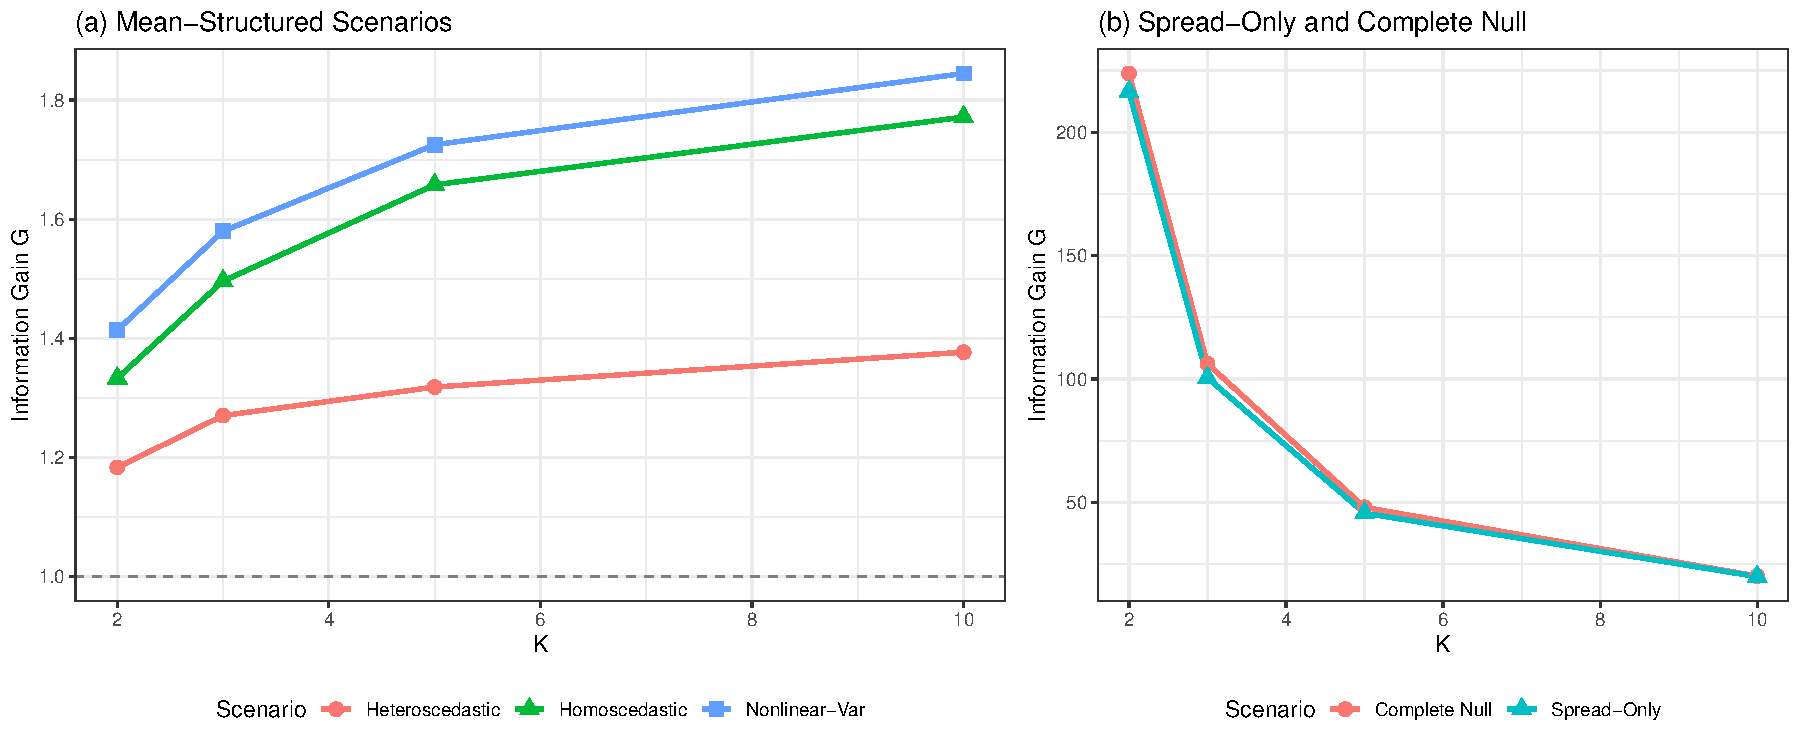
\includegraphics[width=0.95\textwidth]{fig_info_gain_vs_K_v5.pdf}
	\caption{Trace-based gain $G=\mathrm{tr}\{\Sigma_{\mathrm{Int}}^{(\mathrm{Between})}\}/\mathrm{tr}\{\Sigma^{(\mathrm{Between})}\}$ as a function of the number of groups $K$ in the focal simulation setting ($n=500$, $p=10$, 100 Monte Carlo replications per configuration). Panel~(a) reports the mean-structured scenarios; panel~(b) reports the spread-only and complete-null scenarios on a separate vertical scale because the classical between-group trace is close to zero in both cases.}
	\label{fig:info_gain}
\end{figure}

Figure~\ref{fig:eta_improvement} shows the improvement in the mean between-group eta ratio,
\[
\overline{\Delta\eta}_B=\bar{\eta}_B^{(\mathrm{Int})}-\bar{\eta}_B^{(\mathrm{WABA})},
\]
for the heteroscedastic, spread-only, and complete-null scenarios across sample sizes. In the heteroscedastic case, the improvement increases with $K$ and is fairly stable once $n\ge 200$. In the spread-only and complete-null cases, the improvement is much larger overall, but it decreases with $K$ because the classical eta ratio grows slightly as the number of groups increases. The close similarity of the spread-only and complete-null panels reinforces an important interpretive point: improvement in $\eta_B$ alone is also magnitude-inclusive and is not, by itself, a heterogeneity diagnostic.

\begin{figure}[ht]
	\centering
	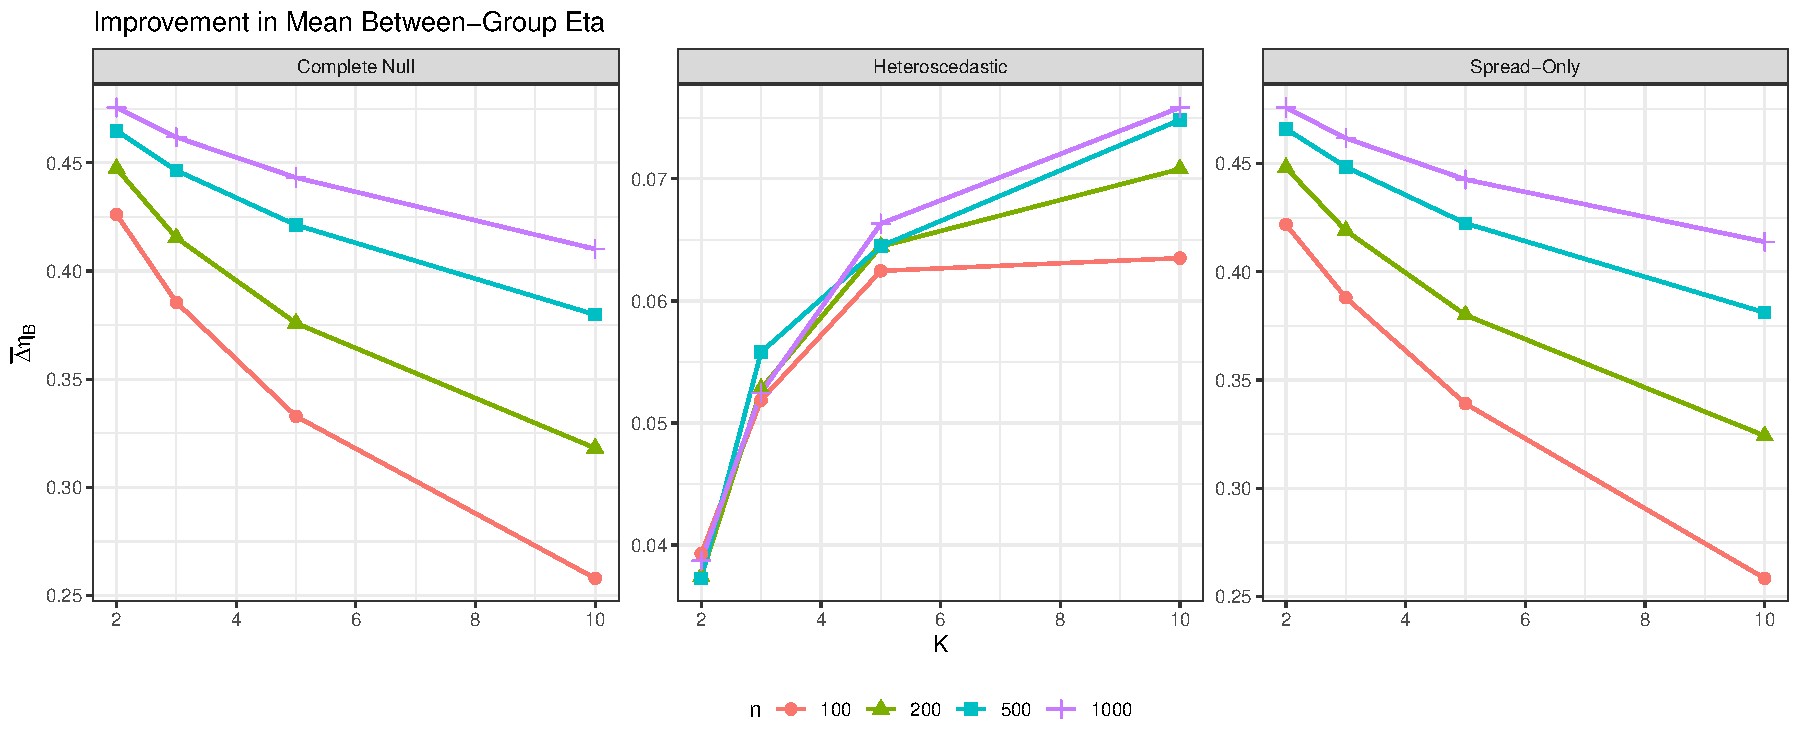
\includegraphics[width=0.95\textwidth]{fig_eta_improvement_v5.pdf}
	\caption{Improvement in the mean between-group eta ratio, $\overline{\Delta\eta}_B=\bar\eta_B^{(\mathrm{Int})}-\bar\eta_B^{(\mathrm{WABA})}$, as a function of the number of groups $K$ and total sample size $n$ for the heteroscedastic, spread-only, and complete-null scenarios ($p=10$, 100 Monte Carlo replications per configuration).}
	\label{fig:eta_improvement}
\end{figure}

Figure~\ref{fig:heatmap} reports the heteroscedastic heatmap of $G$ across $K$ and $p$, averaged over $n$ and Monte Carlo replications. The largest gains occur for small $p$ and large $K$; for example, the mean gain rises from about 1.61 at $(K,p)=(2,2)$ to about 2.08 at $(10,2)$, whereas for $p=50$ it remains near 1.02--1.03 across all $K$.

\begin{figure}[ht]
	\centering
	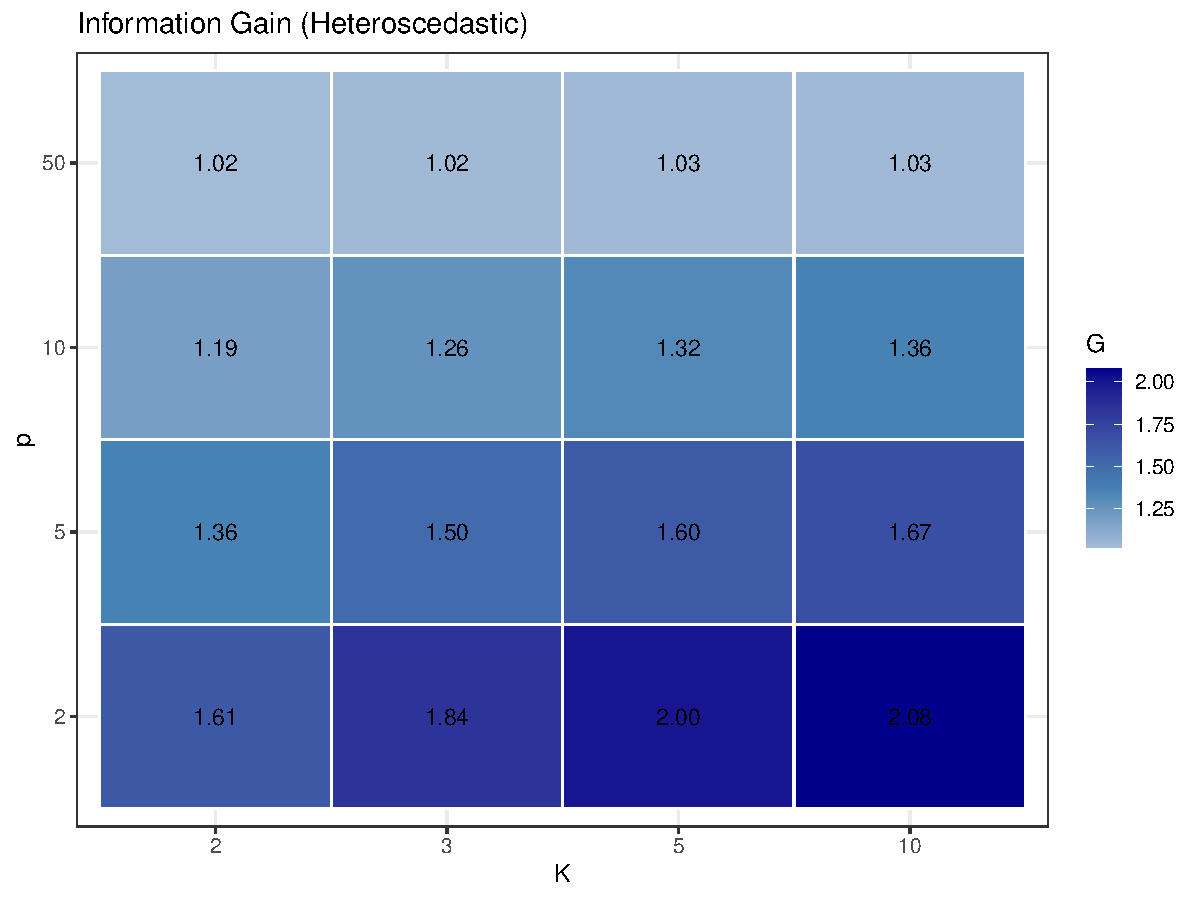
\includegraphics[width=0.70\textwidth]{fig_heatmap_info_gain_v5.pdf}
	\caption{Heatmap of the trace-based gain $G=\mathrm{tr}\{\Sigma_{\mathrm{Int}}^{(\mathrm{Between})}\}/\mathrm{tr}\{\Sigma^{(\mathrm{Between})}\}$ in the heteroscedastic scenario across $(K,p)$ combinations, averaged over $n\in\{100,200,500,1000\}$ and 100 Monte Carlo replications per design point.}
	\label{fig:heatmap}
\end{figure}

%%%%%%%%%%%%%%%%%%%%%%%%%%%%%%%%%%%%%%%%%%%
%                                         %
%%%%%%%%%%%%%%%%%%%%%%%%%%%%%%%%%%%%%%%%%%%

\subsection{Pairwise association decomposition}

For each pair $(X_j,X_{j'})$, we examine the interval-based between-group correlation $r_{\mathrm{Int}}^{(\mathrm{Between})}$, the within-group correlation $r^{(\mathrm{Within})}$, and the corresponding weighted contributions
\[
D_{B,jj'}^{(\mathrm{Int})}
=
\eta_{B,j}^{(\mathrm{Int})}\eta_{B,j'}^{(\mathrm{Int})}r_{\mathrm{Int}}^{(\mathrm{Between})}(X_j,X_{j'}),
\qquad
D_{W,jj'}^{(\mathrm{Int})}
=
\eta_{W,j}^{(\mathrm{Int})}\eta_{W,j'}^{(\mathrm{Int})}r^{(\mathrm{Within})}(X_j,X_{j'}).
\]

Across all heteroscedastic settings, the mean absolute interval-based between-group contribution exceeds the classical mean-based counterpart. At $K=10$, $n=500$, and $p=10$, the mean absolute between-group contribution is 0.500 under I-WABA versus 0.410 under classical WABA, whereas the corresponding within-group contributions are 0.021 and 0.025. Thus the interval augmentation strengthens pairwise between-group dominance while leaving the within-group component essentially unchanged.

The contrast is even sharper in the spread-only scenario. At $K=10$, the mean absolute between-group contribution is 0.244 under I-WABA but only 0.006 under classical WABA, demonstrating that pairwise between-group structure can be induced almost entirely by aligned dispersion differences even when group means are identical.

The complete-null scenario provides the critical counterpoint. At $K=10$, the mean absolute between-group contribution is 0.249 under I-WABA but only 0.007 under classical WABA, even though the data contain neither mean differences nor population-level dispersion heterogeneity. This again shows that Billard's augmentation can generate substantial pairwise between-group magnitude from the radii alone. The attribution and radius-alignment diagnostics are therefore essential for distinguishing the spread-only case, where the radius pattern is genuinely structured, from the complete-null case, where the pairwise gain is primarily magnitude-driven.

The homoscedastic and nonlinear-variance scenarios behave differently. In the homoscedastic control, the interval-based between-group contribution increases because the Billard augmentation carries overall dispersion magnitude, but the heterogeneity-focused diagnostics remain small. In the nonlinear-variance scenario, the between-group contribution increases markedly, reflecting genuine alignment of group means and group radii.

Proposition~\ref{prop:dominance} is therefore most useful on the covariance and weighted-contribution scales, not as a claim that the raw between-group correlation must increase. Remark~\ref{rem:corr_attenuation} gives the exact attenuation criterion. A targeted focal-grid check at the representative configuration $(K,n,p)=(5,500,10)$ makes the empirical frequency of this phenomenon explicit. The mean proportion of pairs with $r_{\mathrm{Int}}^{(\mathrm{Between})}<r^{(\mathrm{Between})}$ is 0.945 in the heteroscedastic scenario, 0.338 in the homoscedastic control, 0.310 in the nonlinear-variance scenario, and essentially zero in the spread-only and complete-null scenarios (both 0.001 after Monte Carlo averaging). When the decrease occurs in the heteroscedastic setting, however, it is numerically mild on average: the mean signed difference $r_{\mathrm{Int}}^{(\mathrm{Between})}-r^{(\mathrm{Between})}$ is about $-0.023$. Thus a slight attenuation of the normalized between-group correlation is compatible with a stronger interval-based pairwise decomposition because the covariance scale and the eta weights both increase.


%%%%%%%%%%%%%%%%%%%%%%%%%%%%%%%%%%%%%%%%%%%
%                                         %
%%%%%%%%%%%%%%%%%%%%%%%%%%%%%%%%%%%%%%%%%%%
\subsection{Alignment diagnostic}

The alignment diagnostic compares the entity-level classification with the pairwise between/within decomposition. In the heteroscedastic scenario, the consistency rate under I-WABA decreases from 35.5\% at $K=2$ to 4.4\% at $K=10$, but it remains uniformly larger than the corresponding classical WABA rate (25.8\%, 8.6\%, 3.4\%, and 0.8\% across $K=2,3,5,10$). This reflects an informative tension: the pairwise decomposition detects strong between-group structure even when the entity-level E-ratio classifies many variables as equivocal.

In the spread-only scenario, the interval-based consistency rate is 0 throughout because the entity-level classifications remain within-group dominant while the pairwise interval-based between-group contribution is substantial. Classical WABA shows the opposite pattern, with high consistency rates (from 98.2\% at $K=2$ to 91.6\% at $K=10$) because both its entity-level and pairwise summaries remain within-group dominated.

The complete-null scenario lies between these extremes. Classical WABA is perfectly self-consistent, with consistency equal to one across all $K$, because both its entity-level and pairwise summaries remain null-like and within-group dominated. Under I-WABA, however, the consistency rate remains only moderate (66.8\%, 66.1\%, 64.3\%, and 62.9\% across $K=2,3,5,10$). This is another manifestation of the fact that pairwise Billard contributions can be nontrivial even under a full null, so alignment between the entity-level E-ratio and the pairwise decomposition should not be expected without the centered-radius diagnostics.

For the homoscedastic and nonlinear-variance scenarios, the consistency rate is 0 for both methods across all $K$. Here again the continuous pairwise contributions are more informative than a strictly categorical interpretation of the entity-level summaries.


%%%%%%%%%%%%%%%%%%%%%%%%%%%%%%%%%%%%%%%%%%%
%                                         %
%%%%%%%%%%%%%%%%%%%%%%%%%%%%%%%%%%%%%%%%%%%
\subsection{Attribution to location and dispersion}\label{sec:sim_level_iv}

Table~\ref{tab:sim_level_iv} summarizes the attribution diagnostics for the focal case. We report the center-only index $\bar E_C^{(\mathrm{Int})}$, the mean dispersion share $\bar\pi_R$, and the heterogeneity-focused index $\bar E_{R,\mathrm{het}}^{(\mathrm{Int})}$. The radius-only index $E_R^{(\mathrm{Int})}$ is omitted because, under the default standard-deviation radius and equal group sizes, it is identically $1/\sqrt{3}$.

\begin{table}[ht]
	\centering
	\caption{Attribution diagnostics for the focal setting ($n=500$, $p=10$). The radius-only index $E_R^{(\mathrm{Int})}$ is constant at $1/\sqrt{3}$ and is therefore omitted.}
	\label{tab:sim_level_iv}
	\begin{tabular}{llccc}
		\toprule
		Scenario & $K$ & $\bar E_C^{(\mathrm{Int})}$ & $\bar\pi_R$ & $\bar E_{R,\mathrm{het}}^{(\mathrm{Int})}$ \\
		\midrule
		Heteroscedastic & 2  & 1.335 & 0.197 & 0.296 \\
		Heteroscedastic & 3  & 1.087 & 0.262 & 0.261 \\
		Heteroscedastic & 5  & 0.994 & 0.291 & 0.248 \\
		Heteroscedastic & 10 & 0.911 & 0.324 & 0.234 \\
		\midrule
		Spread-only     & 2  & 0.035 & 0.994 & 0.337 \\
		Spread-only     & 3  & 0.054 & 0.989 & 0.292 \\
		Spread-only     & 5  & 0.082 & 0.977 & 0.265 \\
		Spread-only     & 10 & 0.130 & 0.949 & 0.249 \\
		\midrule
		Complete-null   & 2  & 0.036 & 0.994 & 0.014 \\
		Complete-null   & 3  & 0.056 & 0.988 & 0.023 \\
		Complete-null   & 5  & 0.084 & 0.977 & 0.034 \\
		Complete-null   & 10 & 0.132 & 0.948 & 0.054 \\
		\midrule
		Homoscedastic   & 2  & 1.001 & 0.251 & 0.015 \\
		Homoscedastic   & 3  & 0.820 & 0.333 & 0.023 \\
		Homoscedastic   & 5  & 0.712 & 0.398 & 0.035 \\
		Homoscedastic   & 10 & 0.657 & 0.437 & 0.054 \\
		\midrule
		Nonlinear-Var   & 2  & 0.899 & 0.294 & 0.258 \\
		Nonlinear-Var   & 3  & 0.759 & 0.368 & 0.219 \\
		Nonlinear-Var   & 5  & 0.678 & 0.422 & 0.194 \\
		Nonlinear-Var   & 10 & 0.628 & 0.460 & 0.182 \\
		\bottomrule
	\end{tabular}
\end{table}

Three patterns are clear. First, the dispersion share alone does not separate genuine heteroscedasticity from magnitude-only controls. The spread-only and complete-null scenarios both have $\bar\pi_R\approx 0.95$--0.99, while the homoscedastic control has a moderate but still substantial dispersion share. Second, the heterogeneity-focused index $\bar E_{R,\mathrm{het}}^{(\mathrm{Int})}$ cleanly separates the two controls from the scenarios with genuine cross-group dispersion heterogeneity. In the complete-null and homoscedastic cases it remains on a low scale (about 0.014--0.054), whereas it is approximately 0.23--0.30 in the heteroscedastic scenario, 0.18--0.26 in the nonlinear-variance scenario, and 0.25--0.34 in the spread-only scenario. Third, the center-only index $\bar E_C^{(\mathrm{Int})}$ tracks mean separation: it is largest in the heteroscedastic and homoscedastic settings, moderate in the nonlinear-variance setting, and close to zero in the spread-only and complete-null scenarios.

\begin{figure}[ht]
	\centering
	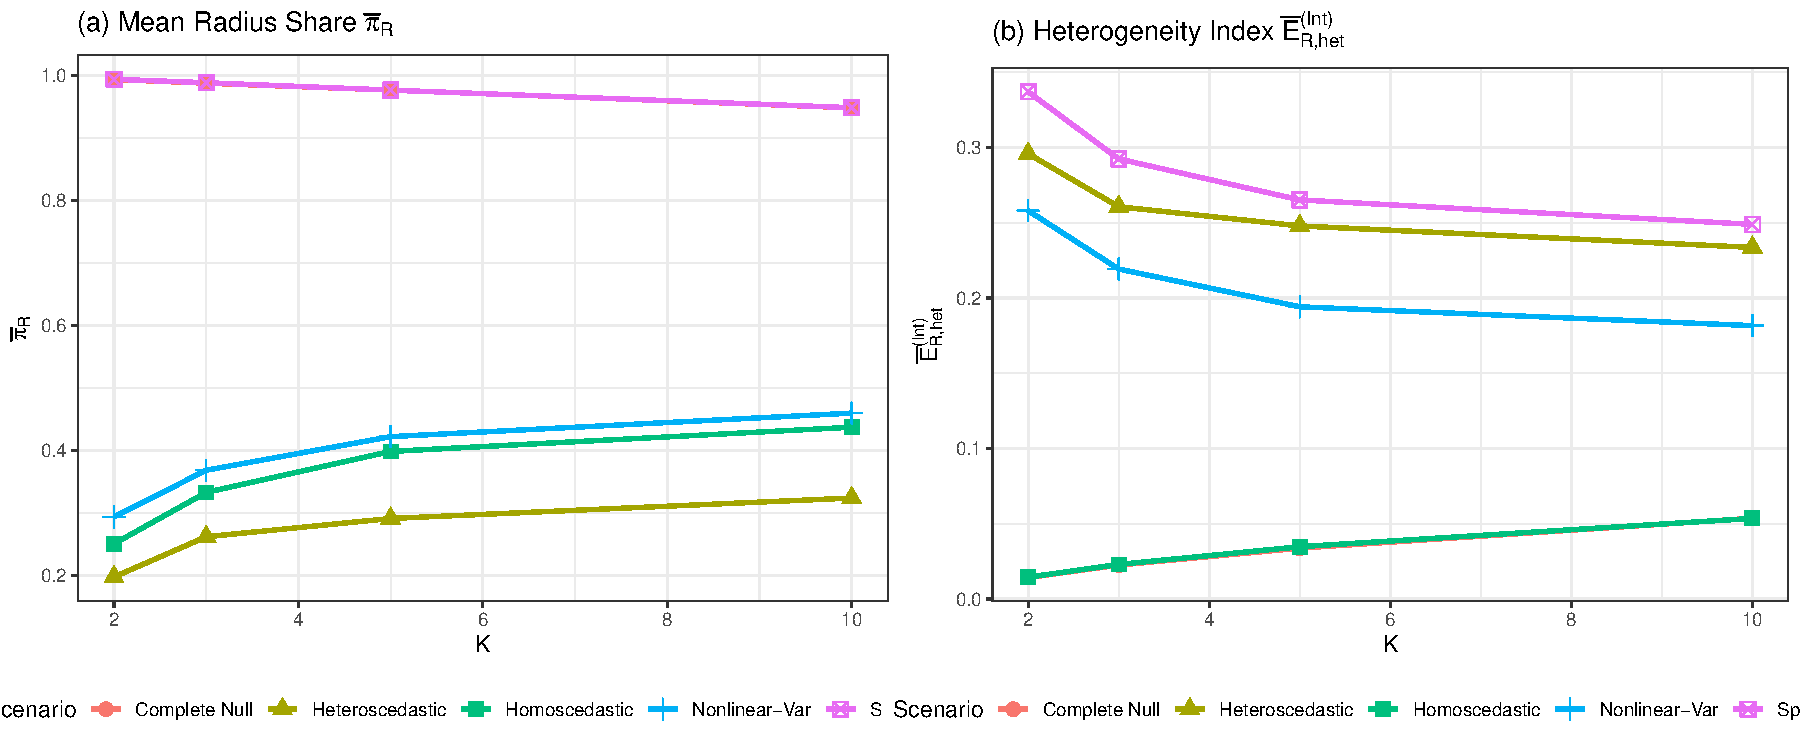
\includegraphics[width=0.95\textwidth]{fig_dispersion_diagnostics_v5.pdf}
	\caption{Attribution diagnostics for the focal simulation setting ($n=500$, $p=10$, 100 Monte Carlo replications per configuration). Panel~(a) shows the mean dispersion share $\bar\pi_R$, the proportion of the interval-based between-group variance attributable to the radius term. Panel~(b) shows the heterogeneity-focused index $\bar E_{R,\mathrm{het}}^{(\mathrm{Int})}$, which removes average radius magnitude and isolates cross-group dispersion heterogeneity.}
	\label{fig:dispersion_diag}
\end{figure}


%%%%%%%%%%%%%%%%%%%%%%%%%%%%%%%%%%%%%%%%%%%
%                                         %
%%%%%%%%%%%%%%%%%%%%%%%%%%%%%%%%%%%%%%%%%%%
\subsection{Dispersion alignment across variables}\label{sec:sim_level_v}

To examine whether group-level dispersion patterns co-move across variables, we report the Billard radius association $\bar r_R^{(\mathrm{Billard})}$ and the signed heterogeneity-based radius correlation $\bar r_{R,\mathrm{het}}$. Because Section~\ref{sec:role_of_K} shows that $r_{R,\mathrm{het}}$ is structurally degenerate when $K=2$, we omit $K=2$ from the graded signed-correlation summaries and figure. In that case the diagnostic reduces to a sign-only measure: in the aligned alternatives it is always positive; in the homoscedastic control the positive and negative signs occur with roughly equal frequency; and in the complete-null calibration the signs are mixed as well, with $P(+)=0.55$ and $P(-)=0.45$.

\begin{table}[ht]
	\centering
	\caption{Dispersion-alignment diagnostics for the focal setting ($n=500$, $p=10$). The signed heterogeneity-based correlation is omitted for $K=2$ because it is structurally degenerate in the two-group case.}
	\label{tab:sim_level_v}
	\begin{tabular}{llcc}
		\toprule
		Scenario & $K$ & $\bar r_R^{(\mathrm{Billard})}$ & $\bar r_{R,\mathrm{het}}$ \\
		\midrule
		Heteroscedastic & 3  & 0.993 & 0.977 \\
		Heteroscedastic & 5  & 0.990 & 0.948 \\
		Heteroscedastic & 10 & 0.983 & 0.896 \\
		\midrule
		Spread-only     & 3  & 0.998 & 0.995 \\
		Spread-only     & 5  & 0.996 & 0.982 \\
		Spread-only     & 10 & 0.991 & 0.952 \\
		\midrule
		Complete-null   & 3  & 0.998 & 0.094 \\
		Complete-null   & 5  & 0.997 & 0.104 \\
		Complete-null   & 10 & 0.992 & 0.114 \\
		\midrule
		Homoscedastic   & 3  & 0.998 & 0.002 \\
		Homoscedastic   & 5  & 0.996 & -0.016 \\
		Homoscedastic   & 10 & 0.991 & -0.001 \\
		\midrule
		Nonlinear-Var   & 3  & 0.998 & 0.993 \\
		Nonlinear-Var   & 5  & 0.996 & 0.974 \\
		Nonlinear-Var   & 10 & 0.991 & 0.918 \\
		\bottomrule
	\end{tabular}
\end{table}

The Billard radius association remains close to one in all scenarios because it is magnitude-inclusive and therefore dominated by the overall scale of the radii. The signed heterogeneity-based correlation is much more informative. It is close to one in the heteroscedastic, spread-only, and nonlinear-variance scenarios, indicating systematic alignment of the group-level dispersion patterns across variables. In the homoscedastic control it fluctuates around zero, confirming that any apparent radius association is driven by overall dispersion magnitude rather than genuine cross-group dispersion alignment. In the complete-null scenario it remains small but positive (about 0.09--0.11), far below the aligned alternatives and again consistent with the interpretation that Billard's magnitude-inclusive association and the centered-radius alignment target are not interchangeable.

\begin{figure}[ht]
	\centering
	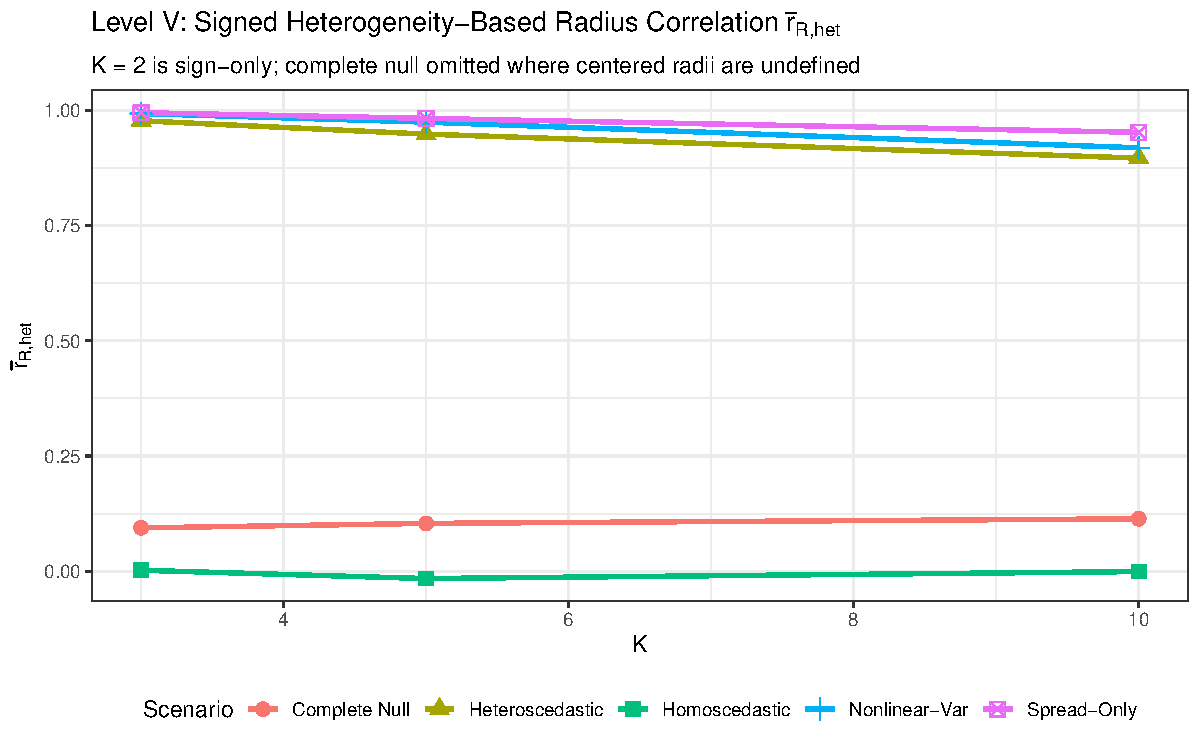
\includegraphics[width=0.70\textwidth]{fig_radius_association_v5.pdf}
	\caption{Mean signed heterogeneity-based radius correlation $\bar r_{R,\mathrm{het}}$ as a function of $K$ in the focal simulation setting ($n=500$, $p=10$, 100 Monte Carlo replications per configuration). The diagnostic summarizes alignment of centered group radii across variables. The case $K=2$ is omitted because the centered-radius correlation is structurally degenerate there and reduces to a sign-only summary.}
	\label{fig:radius_assoc}
\end{figure}


%%%%%%%%%%%%%%%%%%%%%%%%%%%%%%%%%%%%%%%%%%%
%                                         %
%%%%%%%%%%%%%%%%%%%%%%%%%%%%%%%%%%%%%%%%%%%

\subsection{Sensitivity to sample size and dimensionality}

%%%%%%%%%%%%%%%%%%%%%%
%                    %
%%%%%%%%%%%%%%%%%%%%%%
\subsubsection{Sample-size sensitivity}

Fixing $K=5$ and $p=10$, the heteroscedastic scenario shows stable gains across sample sizes: $G$ ranges from 1.304 at $n=100$ to 1.328 at $n=1000$, $\Delta_{\mathrm{tr}}$ remains near 6.24--6.49, and $\bar E_{R,\mathrm{het}}^{(\mathrm{Int})}$ remains close to 0.24--0.25. The signed heterogeneity-based radius correlation strengthens from 0.868 at $n=100$ to 0.954 at $n=1000$, reflecting improved estimation of the group radii.

The homoscedastic control behaves differently. The gain remains around 1.59--1.66 because Billard's augmentation includes overall dispersion magnitude, but $\bar E_{R,\mathrm{het}}^{(\mathrm{Int})}$ decreases from 0.078 at $n=100$ to 0.024 at $n=1000$, and the signed heterogeneity-based radius correlation stays near zero. Thus the heterogeneity-focused diagnostics converge toward the correct null pattern even though the magnitude-inclusive Billard augmentation remains positive.

The nonlinear-variance scenario is again stable, with $G$ rising from 1.656 to 1.740, $\Delta_{\mathrm{tr}}$ remaining near 3.57--3.73, and $\bar r_{R,\mathrm{het}}$ increasing from 0.869 to 0.987. In the spread-only scenario, the gain ratio $G$ increases sharply with $n$ because the classical between-group trace in the denominator remains close to zero, whereas the heterogeneity-focused diagnostics are stable: $\bar E_{R,\mathrm{het}}^{(\mathrm{Int})}$ stays near 0.26, $\Delta_{\mathrm{tr}}$ stays near 12.2--13.0, and $\bar r_{R,\mathrm{het}}$ rises from 0.928 to 0.990.

The complete-null scenario behaves like spread-only with respect to the ratio $G$ but not with respect to heterogeneity. At $K=5$, $G$ increases from 9.571 at $n=100$ to 94.036 at $n=1000$, even though the additive gain stays nearly flat ($\Delta_{\mathrm{tr}}=3.159$ to 3.315). Over the same range, $\bar E_{R,\mathrm{het}}^{(\mathrm{Int})}$ declines from 0.077 to 0.024 and $\bar r_{R,\mathrm{het}}$ remains on a low scale around 0.10. This is precisely the pattern expected when the ratio is driven by a shrinking classical denominator rather than by strengthening dispersion heterogeneity.

%%%%%%%%%%%%%%%%%%%%%%
%                    %
%%%%%%%%%%%%%%%%%%%%%%
\subsubsection{Dimensionality sensitivity}

Fixing $K=5$ and $n=500$, the redesigned nested-template experiment shows two distinct patterns. In the heteroscedastic scenario, the trace-based gain decreases from 1.996 at $p=2$ to 1.029 at $p=50$, and the dispersion share decreases from 0.499 to 0.088. By contrast, the heterogeneity-focused summaries are remarkably stable:
\[
\bar E_{R,\mathrm{het}}^{(\mathrm{Int})}\approx 0.248
\qquad\text{and}\qquad
\bar r_{R,\mathrm{het}}\approx 0.946\text{--}0.948
\]
throughout. Thus the decline in $G$ reflects the scaling of the trace ratio under increasing dimension, not the disappearance of heterogeneous dispersion.

The complete-null scenario adds a new calibration pattern. At $K=5$, $G$ declines only moderately with dimension, from 56.068 at $p=2$ to 45.093 at $p=50$, while the additive gain grows strongly from $\Delta_{\mathrm{tr}}=0.661$ to $16.538$. At the same time, the heterogeneity-focused summaries remain nearly unchanged and small: $\bar E_{R,\mathrm{het}}^{(\mathrm{Int})}\approx 0.034$ throughout, and the signed radius correlation stays on a low scale relative to the aligned alternatives. Thus dimensional growth can substantially change the absolute Billard contribution without generating evidence of genuine dispersion heterogeneity.

The homoscedastic, nonlinear-variance, and spread-only scenarios are more stable across $p$. In the homoscedastic control, $G$ remains near 1.65 and $\bar E_{R,\mathrm{het}}^{(\mathrm{Int})}$ remains near 0.035, while the signed heterogeneity-based radius correlation stays near zero. In the nonlinear-variance scenario, both $G$ and the heterogeneity-focused diagnostics are nearly invariant to $p$. In the spread-only scenario, $G$ remains very large (approximately 43--57), $\bar\pi_R$ remains about 0.977, and $\bar r_{R,\mathrm{het}}$ remains about 0.982.

%%%%%%%%%%%%%%%%%%%%%%%%%%%%%%%%%%%%%%%%%%%
%                                         %
%%%%%%%%%%%%%%%%%%%%%%%%%%%%%%%%%%%%%%%%%%%
\subsection{Targeted comparator results}\label{sec:sim_comparator}

Table~\ref{tab:sim_comparator} reports the targeted comparator experiment for the spread-only and complete-null scenarios. Classical WABA never identifies any between-group dominant variables in either scenario: the mean number of between-group dominant variables is zero and the familywise probability of at least one such classification is also zero throughout. The comparison is therefore between I-WABA's interval-based decomposition and two simpler adjunct procedures: Brown--Forsythe screening and Welch-type one-way heteroscedastic ANOVA.

Brown--Forsythe behaves exactly as expected. In the complete-null scenario, its per-variable rejection rate is near the nominal level (0.003--0.007), with familywise ``any reject'' rates of 0.03--0.07. In the spread-only scenario, by contrast, Brown--Forsythe rejects in every variable and every replication. Welch's procedure does \emph{not} distinguish the two scenarios: its per-variable rejection rate remains close to 0.05 in both, while the familywise ``any reject'' rate ranges from 0.30 to 0.45 under complete null and from 0.36 to 0.42 under spread-only. This familywise rate should not be read as evidence of mean structure; it is simply the probability of at least one false positive among ten unadjusted mean tests.

The I-WABA summaries clarify what the comparators do and do not reveal. In both scenarios, the interval-based mean eta is about 0.50, so the Billard-based augmentation alone does not distinguish complete null from spread-only. The heterogeneity-focused index does: $\bar E_{R,\mathrm{het}}^{(\mathrm{Int})}$ is only 0.014--0.054 under complete null but 0.250--0.336 under spread-only. Thus Brown--Forsythe and $E_{R,\mathrm{het}}^{(\mathrm{Int})}$ are broadly concordant as heterogeneity detectors, whereas Welch addresses a different null entirely and classical WABA remains blind to the interval-based radius contribution.

\begin{table}[ht]
	\centering
	\caption{Targeted comparator experiment for the focal setting ($n=500$, $p=10$, 100 replications). ``BF rate'' and ``Welch rate'' are per-variable rejection rates at level 0.05; ``Any'' is the familywise probability of at least one rejection among the 10 variables. Classical WABA yields no between-group dominant variables in either scenario.}
	\label{tab:sim_comparator}
	\begin{tabular}{llcccccc}
		\toprule
		Scenario & $K$ & BF rate & BF any & Welch rate & Welch any & $\bar\eta_B^{\mathrm{I\text{-}WABA}}$ & $\bar E_{R,\mathrm{het}}^{(\mathrm{Int})}$ \\
		\midrule
		Complete-null & 2  & 0.003 & 0.03 & 0.059 & 0.35 & 0.501 & 0.014 \\
		Complete-null & 3  & 0.007 & 0.07 & 0.047 & 0.30 & 0.502 & 0.023 \\
		Complete-null & 5  & 0.005 & 0.05 & 0.059 & 0.45 & 0.505 & 0.034 \\
		Complete-null & 10 & 0.004 & 0.04 & 0.058 & 0.39 & 0.510 & 0.054 \\
		\midrule
		Spread-only   & 2  & 1.000 & 1.00 & 0.047 & 0.36 & 0.501 & 0.336 \\
		Spread-only   & 3  & 1.000 & 1.00 & 0.049 & 0.42 & 0.502 & 0.293 \\
		Spread-only   & 5  & 1.000 & 1.00 & 0.047 & 0.37 & 0.504 & 0.265 \\
		Spread-only   & 10 & 1.000 & 1.00 & 0.061 & 0.42 & 0.511 & 0.250 \\
		\bottomrule
	\end{tabular}
\end{table}

%%%%%%%%%%%%%%%%%%%%%%%%%%%%%%%%%%%%%%%%%%%
%                                         %
%%%%%%%%%%%%%%%%%%%%%%%%%%%%%%%%%%%%%%%%%%%
\subsection{Inferential performance}\label{sec:sim_inference}

We next examine the inferential procedures of Section~\ref{sec:inference}. The focus is on three targets: the entity-level dominance contrast $\delta_1^{(E)}$, the pairwise dominance contrast $\delta_{12}^{(A)}$, and the heterogeneity-based radius correlation $r_{R,\mathrm{het}}(X_1,X_2)$. We evaluate bootstrap coverage and interval length, and then the size and power of the Brown--Forsythe test for dispersion heterogeneity and the bootstrap test for $r_{R,\mathrm{het}}(X_1,X_2)=0$.

\begin{table}[ht]
	\centering
	\caption{Empirical coverage and mean interval length for 95\% within-group bootstrap intervals. Each entry is coverage followed by mean interval length in brackets.}
	\label{tab:sim_inference_coverage}
	\begin{tabular}{llccc}
		\toprule
		Scenario & $n$ & $\delta_1^{(E)}$ & $\delta_{12}^{(A)}$ & $r_{R,\mathrm{het}}(X_1,X_2)$ \\
		\midrule
		Aligned heteroscedastic & 100 & 0.880 [0.842] & 0.960 [0.164] & 0.600 [1.049] \\
		Homoscedastic null      & 100 & 0.897 [0.774] & 0.957 [0.159] & -- \\
		Orthogonal heterogeneity& 100 & 0.850 [0.885] & 0.933 [0.167] & 0.967 [1.182] \\
		\midrule
		Aligned heteroscedastic & 500 & 0.933 [0.383] & 0.947 [0.068] & 0.873 [0.438] \\
		Homoscedastic null      & 500 & 0.933 [0.357] & 0.947 [0.066] & -- \\
		Orthogonal heterogeneity& 500 & 0.933 [0.406] & 0.943 [0.070] & 0.957 [0.658] \\
		\bottomrule
	\end{tabular}
\end{table}

Bootstrap coverage is satisfactory for the dominance contrasts once $n=500$, with empirical coverage near 0.94 for both $\delta_1^{(E)}$ and $\delta_{12}^{(A)}$ across all scenarios. At $n=100$, however, the gaps are nontrivial: coverage for $\delta_1^{(E)}$ falls to 0.880 in the aligned heteroscedastic scenario and to 0.850 in the orthogonal-heterogeneity scenario. The heterogeneity-based radius correlation is more challenging still. In the aligned heteroscedastic scenario its coverage is only 0.600 at $n=100$ and 0.873 at $n=500$, whereas in the orthogonal-heterogeneity scenario, where the true target is near zero, coverage is 0.967 at $n=100$ and 0.957 at $n=500$. This pattern is consistent with a boundary effect: bootstrap intervals for $r_{R,\mathrm{het}}$ are materially harder when the true correlation is close to one than when it is near the interior null.

For practical interpretation, it is useful to translate total sample size into approximate per-group sample size. In this experiment $K=5$, so $n=100$ corresponds to roughly $n_k\approx 20$ observations per group and $n=500$ to roughly $n_k\approx 100$ per group under balance. The results suggest that entity-level and pairwise dominance contrasts are only cautiously interpretable at $n_k\approx 20$, with noticeable undercoverage already present for $\delta_1^{(E)}$. Inference for signed dispersion alignment is unreliable in that regime and should be regarded as exploratory. By $n_k\approx 100$, dominance-contrast inference is much better calibrated and the bootstrap procedure for $r_{R,\mathrm{het}}$ is substantially more reliable, although boundary-adjacent targets remain harder than interior ones. In practice, we therefore view $n_k\approx 20$ as a lower bound for exploratory use of the bootstrap layer and $n_k\approx 100$ as a more defensible regime for inference under roughly regular within-group sampling.

To probe robustness beyond the baseline Gaussian balanced design, we added a small sensitivity block with two departures: standardized log-normal within-group errors with $\mathrm{sdlog}=1$ under balance, and a Gaussian design with an approximately $10{:}1$ group-size ratio. Table~\ref{tab:sim_inference_robustness} summarizes the results. The qualitative message is asymmetric. Group-size imbalance alone is much less harmful than skewness: under the unbalanced Gaussian design, coverage for $\delta_1^{(E)}$, $\delta_{12}^{(A)}$, and $r_{R,\mathrm{het}}$ is $(0.88,0.95,0.85)$ at $n=100$ and improves to $(0.95,0.94,0.94)$ at $n=500$. By contrast, moderate log-normal skewness substantially degrades the bootstrap layer, especially for signed dispersion alignment: even at $n=500$, the corresponding coverages are only $(0.76,0.80,0.37)$. Thus the fixed-$K$ bootstrap layer appears reasonably stable to imbalance in the present design, but considerably less robust to skewed within-group sampling, particularly for heterogeneity-based correlation targets.

\begin{table}[ht]
	\centering
	\caption{Robustness of 95\% within-group bootstrap intervals under two departures from the baseline Gaussian balanced inferential design. The skewed setting uses standardized log-normal within-group errors with $\mathrm{sdlog}=1$ and balanced groups; the unbalanced setting uses Gaussian within-group errors with group-size patterns $(5,9,14,24,48)$ at $n=100$ and $(24,48,71,119,238)$ at $n=500$, approximating a $10{:}1$ ratio. Entries are empirical coverage followed by mean interval length in brackets over 100 Monte Carlo replications with 199 bootstrap resamples.}
	\label{tab:sim_inference_robustness}
	\begin{tabular}{llccc}
		\toprule
		Setting & $n$ & $\delta_1^{(E)}$ & $\delta_{12}^{(A)}$ & $r_{R,\mathrm{het}}(X_1,X_2)$ \\
		\midrule
		Log-normal, balanced   & 100 & 0.610 [0.843] & 0.790 [0.291] & 0.360 [1.358] \\
		Log-normal, balanced   & 500 & 0.760 [0.588] & 0.800 [0.166] & 0.370 [1.285] \\
		Gaussian, unbalanced   & 100 & 0.880 [0.774] & 0.950 [0.126] & 0.850 [0.911] \\
		Gaussian, unbalanced   & 500 & 0.950 [0.360] & 0.940 [0.052] & 0.940 [0.554] \\
		\bottomrule
	\end{tabular}
\end{table}

\begin{table}[ht]
	\centering
	\caption{Empirical size and power for the inferential experiment. The Brown--Forsythe test targets equal within-group variances for $X_1$. The bootstrap test targets $H_0:r_{R,\mathrm{het}}(X_1,X_2)=0$.}
	\label{tab:sim_inference_power}
	\begin{tabular}{llcc}
		\toprule
		Scenario & $n$ & Brown--Forsythe & Bootstrap test for $r_{R,\mathrm{het}}$ \\
		\midrule
		Aligned heteroscedastic & 100 & 0.677 (power) & 0.357 (power) \\
		Homoscedastic null      & 100 & 0.020 (size)  & -- \\
		Orthogonal heterogeneity& 100 & 0.640 (power) & 0.033 (size) \\
		\midrule
		Aligned heteroscedastic & 500 & 1.000 (power) & 0.993 (power) \\
		Homoscedastic null      & 500 & 0.047 (size)  & -- \\
		Orthogonal heterogeneity& 500 & 1.000 (power) & 0.043 (size) \\
		\bottomrule
	\end{tabular}
\end{table}

The Brown--Forsythe test has well-controlled size under the homoscedastic null and good power even at $n=100$; by $n=500$ its power is effectively one. The bootstrap test for the heterogeneity-based radius correlation also controls size well in the orthogonal-heterogeneity scenario and achieves very high power at $n=500$, but it is much less powerful at $n=100$. These results also clarify the relationship between the Brown--Forsythe null and the I-WABA targets. Brown--Forsythe addresses variablewise equality of within-group variances, which is an operational surrogate for the null $V_{R,\mathrm{het}}^{(j)}=0$ but not a direct test of the centered-radius contribution itself. Accordingly, we use Brown--Forsythe as a screening device for the presence of heterogeneity and retain $E_{R,\mathrm{het}}^{(\mathrm{Int})}$ and $r_{R,\mathrm{het}}$ as the decomposition-scale effect summaries.


%%%%%%%%%%%%%%%%%%%%%%%%%%%%%%%%%%%%%%%%%%%
%                                         %
%%%%%%%%%%%%%%%%%%%%%%%%%%%%%%%%%%%%%%%%%%%
\subsection{Summary of simulation findings}

The simulations support eight main conclusions.

First, the interval-based augmentation consistently increases the entity-level between-group signal whenever within-group dispersion differs across groups. This is most striking in the spread-only scenario, where classical WABA is nearly blind to the between-group structure but I-WABA produces substantial between-group eta ratios.

Second, the homoscedastic and complete-null controls show why Billard-based gains cannot be interpreted in isolation. A positive $G$, a large $\bar\eta_B^{(\mathrm{Int})}$, or a large radius share $\pi_R$ may be driven largely by dispersion magnitude even when the heterogeneity-focused summaries remain small.

Third, the additive trace gain $\Delta_{\mathrm{tr}}$ is a useful companion to the ratio $G$. In scenarios with near-zero classical between-group trace, especially spread-only and complete null, $\Delta_{\mathrm{tr}}$ is far more stable and therefore easier to interpret as the absolute contribution of the radius augmentation.

Fourth, at the pairwise level, the interval-based between-group contribution can dominate even when the entity-level E-ratio remains equivocal or within-group dominant, and that strengthening need not coincide with a larger raw between-group correlation. In the representative $(K,n,p)=(5,500,10)$ runs, the proportion of pairs with $r_{\mathrm{Int}}^{(\mathrm{Between})}<r^{(\mathrm{Between})}$ is about 0.95 in the heteroscedastic scenario but essentially zero in the spread-only and complete-null scenarios; when it occurs in the heteroscedastic case, the average attenuation is small (about $-0.023$). The alignment diagnostic therefore usefully distinguishes settings in which the entity-level and pairwise summaries tell different stories.

Fifth, the attribution diagnostics are essential for interpretation under Billard's formulation. The dispersion share $\pi_R$ alone cannot distinguish heterogeneous dispersion from homogeneous or null magnitude effects. The heterogeneity-focused index $E_{R,\mathrm{het}}^{(\mathrm{Int})}$ is the key diagnostic for that distinction.

Sixth, the targeted comparator experiment shows that I-WABA is complementary to simpler procedures rather than redundant with them. Brown--Forsythe detects variablewise spread heterogeneity, Welch addresses mean differences under unequal variances, and classical WABA remains mean-only; none of these provides the integrated within/between decomposition delivered by I-WABA.

Seventh, the heterogeneity-based radius correlation is much more informative than the magnitude-inclusive Billard radius association, and the case $K=2$ is structurally special. For two-group designs, signed radius alignment should be treated as a sign-only diagnostic rather than as a graded correlation summary. The inferential experiment further shows that the bootstrap layer is exploratory at per-group sizes around 20 and becomes materially more reliable only at per-group sizes around 100 under roughly regular within-group sampling.

Eighth, the new robustness block shows that not all departures from the baseline design are equally consequential. In the present fixed-$K$ setting, Gaussian group-size imbalance is comparatively mild, whereas moderate log-normal skewness substantially degrades coverage for the dominance contrasts and especially for signed dispersion alignment. This reinforces two practical recommendations: first, heterogeneity-focused inference should be treated as exploratory when within-group sampling is strongly skewed, and second, sensitivity to robust radius choices should be checked whenever skewness or outliers are scientifically plausible.



%%%%%%%%%%%%%%%%%%%%%%%%%%%%%%%%%%%%%%%%%%%%%%%%%%%%%%%%%%%%%%%%%%%%%%%%%%%%%%%%
%% 5. Real Data Analysis
%%%%%%%%%%%%%%%%%%%%%%%%%%%%%%%%%%%%%%%%%%%%%%%%%%%%%%%%%%%%%%%%%%%%%%%%%%%%%%%%
\section{Real Data Analysis}\label{sec:realdata}

We apply the interval-augmented decomposition to two datasets from different scientific domains. The first is a multilevel organizational dataset in which the central question is whether interval augmentation changes the level-of-analysis interpretation. The second is a multiclass HDLSS gene-expression dataset in which the central question is whether cross-group dispersion heterogeneity is present at scale and whether it survives multiplicity-adjusted screening. In both analyses, the revised diagnostics allow us to distinguish three conceptually different features: overall dispersion magnitude, genuine cross-group dispersion heterogeneity, and signed dispersion alignment across variables.

\subsection{Dataset 1: Bliese--Halverson Military Leadership Data ($K=99$)}\label{sec:data_bh1996}

The \texttt{bh1996} dataset from the \texttt{multilevel} package \citep{Bliese2000pkg} contains $n=7{,}382$ soldiers nested in $K=99$ Army companies, with four variables: vertical cohesion (COHES), leadership climate (LEAD), psychological well-being (WBEING), and weekly work hours (HRS). The dataset has long served as a benchmark for multilevel decomposition and level-of-analysis questions \citep{bliese1996individual,bliese2002benchmarking}. It is particularly useful here because the number of groups is large and the variables plausibly differ not only in company means but also in within-company variability. The empirical group-size distribution is not sparse: company sizes range from 15 to 226, with quartiles 43.5 and 94, median 64, and mean 74.6. Thus most companies contribute dozens of observations. At the same time, because $K=99$ is itself large, the formal fixed-$K$ asymptotic regime of Section~\ref{sec:inference} is not the most natural theoretical limit for this dataset; a large-$K$ treatment would be more natural. We therefore treat the inferential layer in this subsection as exploratory: the bootstrap intervals and tests below are practically informative approximations in a design with many groups and moderate-to-large typical $n_k$, but they are not presented as direct empirical validation of the fixed-$K$ theory.

\subsubsection{Entity-level and pairwise decomposition}

At the entity level, the updated SD-radius analysis preserves the main descriptive conclusion of the earlier draft: all four variables remain within-group dominant under both classical WABA and I-WABA. However, the interval augmentation is substantial. The variablewise between-group eta values increase from $(0.238, 0.371, 0.236, 0.379)$ under classical WABA to $(0.531, 0.575, 0.531, 0.578)$ under I-WABA for COHES, LEAD, WBEING, and HRS, respectively. Averaged across the four variables, the mean between-group eta rises from 0.306 to 0.554, with a trace-based gain of $G=3.351$ and a trace-weighted radius proportion of 0.702. Thus the interval representation adds a large amount of between-group signal even though it does not overturn the variable-level classification. Table~\ref{tab:bh1996_waba1} reports the variablewise details.

\begin{table}[ht]
	\centering
	\caption{Bliese--Halverson (\texttt{bh1996}) data: entity-level decomposition under the default SD radius. $\eta_B$ and $\eta_W$ are the classical between-group and within-group eta ratios, $E$ is the corresponding E-ratio, and the interval-based quantities are reported with superscript \((\mathrm{Int})\). The raw variance components $V_C$, $V_R$, and $V_W$ remain on the original measurement scale of each variable and are therefore not directly comparable across variables; substantive cross-variable comparisons should rely on the scale-free ratios.}
	\label{tab:bh1996_waba1}
	\begin{tabular}{lcccccccccc}
		\toprule
		Variable & $\eta_B$ & $\eta_W$ & $E$ & $\eta_B^{(\mathrm{Int})}$ & $\eta_W^{(\mathrm{Int})}$ & $E^{(\mathrm{Int})}$ & $\Delta\eta_B$ & $V_C$ & $V_R$ & $V_W$ \\
		\midrule
		COHES  & 0.238 & 0.971 & 0.245 & 0.531 & 0.847 & 0.627 & 0.294 & 0.043 & 0.237 & 0.712 \\
		LEAD   & 0.371 & 0.929 & 0.399 & 0.575 & 0.818 & 0.702 & 0.204 & 0.082 & 0.171 & 0.514 \\
		WBEING & 0.236 & 0.972 & 0.243 & 0.531 & 0.847 & 0.626 & 0.295 & 0.046 & 0.260 & 0.779 \\
		HRS    & 0.379 & 0.925 & 0.409 & 0.578 & 0.816 & 0.708 & 0.199 & 0.741 & 1.474 & 4.423 \\
		\bottomrule
	\end{tabular}
\end{table}

The pairwise decomposition remains the clearest practical manifestation of the interval augmentation. Under classical WABA, all six pairs are within-group dominant. Under I-WABA, four of the six pairs flip to between-group dominance: COHES--WBEING, COHES--HRS, LEAD--HRS, and WBEING--HRS. Only COHES--LEAD and LEAD--WBEING remain within-group dominant. This pairwise pattern is unchanged under the IQR-radius sensitivity analysis discussed below, so the main level-of-analysis conclusion is not an artifact of the default SD radius. Table~\ref{tab:bh1996_waba2} reports the SD-radius pairwise results.

\begin{table}[ht]
	\centering
	\caption{Bliese--Halverson (\texttt{bh1996}) data: pairwise decomposition under the default SD radius. The weighted between-group and within-group contributions are compared on the covariance-decomposition scale.}
	\label{tab:bh1996_waba2}
	\resizebox{\textwidth}{!}{%
		\begin{tabular}{lcccccccc}
			\toprule
			Pair & $r^{(Between)}$ & $r^{(Within)}$ & $r_{\mathrm{Int}}^{(Between)}$ & $D_{B}^{(\mathrm{WABA})}$ & $D_{W}^{(\mathrm{WABA})}$ & $D_{B}^{(\mathrm{Int})}$ & $D_{W}^{(\mathrm{Int})}$ & Dominance (I-WABA) \\
			\midrule
			COHES--LEAD   & 0.653 & 0.405 & 0.897 & 0.058 & 0.366 & 0.274 & 0.281 & Within \\
			COHES--WBEING & 0.271 & 0.238 & 0.884 & 0.015 & 0.225 & 0.249 & 0.171 & Between \\
			COHES--HRS    & $-0.028$ & $-0.111$ & 0.729 & $-0.002$ & $-0.100$ & 0.224 & $-0.077$ & Between \\
			LEAD--WBEING  & 0.532 & 0.420 & 0.870 & 0.047 & 0.379 & 0.265 & 0.291 & Within \\
			LEAD--HRS     & $-0.300$ & $-0.108$ & 0.558 & $-0.042$ & $-0.093$ & 0.185 & $-0.072$ & Between \\
			WBEING--HRS   & $-0.712$ & $-0.111$ & 0.578 & $-0.064$ & $-0.100$ & 0.177 & $-0.077$ & Between \\
			\bottomrule
		\end{tabular}%
	}
\end{table}

The alignment diagnostic remains informative rather than problematic. Under classical WABA, the entity-level and pairwise conclusions agree for all six pairs. Under I-WABA, the consistency rate drops to $2/6=33.3\%$, because the entity-level E-ratios remain below one while the pairwise decomposition reveals between-group dominance for four pairs. This tension is precisely the phenomenon that the interval augmentation is designed to expose: the variablewise signal can remain individually weak while the joint pairwise between-group structure becomes substantial.

\subsubsection{Attribution, inference, and sensitivity to radius and scale}

The revised Level~IV diagnostics show why the large gain in \texttt{bh1996} should not be interpreted too quickly as strong heteroscedasticity. Because $K=99$ lies outside the fixed-$K$ asymptotic regime of Section~\ref{sec:inference}, the custom I-WABA bootstrap intervals cited below are reported only as exploratory approximations. The mean variablewise radius share is 0.760 and the trace-weighted radius proportion is 0.702, so the augmented between-group variance is dominated by the radius contribution. However, the heterogeneity-focused index is much smaller, with mean $\bar E_{R,\mathrm{het}}^{(\mathrm{Int})}=0.070$. At the variable level, $E_{R,\mathrm{het}}^{(\mathrm{Int})}$ is 0.053 for COHES, 0.053 for LEAD, 0.056 for WBEING, and 0.120 for HRS. Thus HRS shows the strongest genuine company-level dispersion heterogeneity, while the other three variables exhibit only mild heterogeneity despite their large radius shares. Table~\ref{tab:bh1996_level4} summarizes these diagnostics together with the multiplicity-adjusted Brown--Forsythe results.

\begin{table}[ht]
	\centering
	\caption{Bliese--Halverson (\texttt{bh1996}) data: Level~IV attribution diagnostics under the default SD radius. The radius-only index $E_R^{(\mathrm{Int})}$ is omitted because, under the default standard-deviation radius, it is constant at $1/\sqrt{3}$. The final column reports the Benjamini--Hochberg adjusted Brown--Forsythe $q^\dagger$-value for testing equality of within-company variances. \(^\dagger\) In this large-$K$ application, the inferentially interpreted quantities in this subsection, including the surrounding custom I-WABA bootstrap interval statements, are reported only as exploratory approximations because $K=99$ lies outside the fixed-$K$ regime of Section~\ref{sec:inference}.}
	\label{tab:bh1996_level4}
	\begin{tabular}{lcccc}
		\toprule
		Variable & $\pi_R$ & $E_C^{(\mathrm{Int})}$ & $E_{R,\mathrm{het}}^{(\mathrm{Int})}$ & BF--BH $q^\dagger$ \\
		\midrule
		COHES  & 0.848 & 0.245 & 0.053 & 0.0225 \\
		LEAD   & 0.676 & 0.399 & 0.053 & 0.0853 \\
		WBEING & 0.850 & 0.243 & 0.056 & 0.0137 \\
		HRS    & 0.666 & 0.409 & 0.120 & $6.33\times 10^{-11}$ \\
		\bottomrule
	\end{tabular}
\end{table}

A useful practical rule emerges from Table~\ref{tab:bh1996_level4}. Brown--Forsythe testing answers whether unequal within-company variances are detectable, whereas $E_{R,\mathrm{het}}^{(\mathrm{Int})}$ answers how much that heterogeneity contributes to the interval-augmented between-group decomposition. Thus COHES and WBEING show statistically detectable variance heterogeneity but only small structural contribution to I-WABA, with $E_{R,\mathrm{het}}^{(\mathrm{Int})}\approx 0.05$. HRS is the only variable for which both the variance test and the attribution diagnostic point clearly in the same direction. LEAD, by contrast, has a similarly small $E_{R,\mathrm{het}}^{(\mathrm{Int})}$ but does not reach Brown--Forsythe significance after multiplicity adjustment. In all four cases, the within-group bootstrap intervals for the entity-level dominance contrast $\delta_j^{(E)}$ remain strictly negative, but these intervals are outside the fixed-$K$ regime and are therefore reported only as exploratory approximations. The variable-level conclusion of within-group dominance is not overturned even under that approximate uncertainty assessment.

At the pairwise level, the bootstrap intervals for $\delta_{jj'}^{(A)}$ are strictly positive for the four pairs that flip to between-group dominance, strictly negative for LEAD--WBEING, and include zero for COHES--LEAD, but every such interval statement is again outside the fixed-$K$ regime and is therefore exploratory. Under the default SD radius, the signed Level~V results are also uniformly positive: the Billard radius association ranges from 0.978 to 0.994, whereas the signed heterogeneity-based radius correlation ranges from 0.221 to 0.363 with mean 0.260, and all six SD-based bootstrap intervals for $r_{R,\mathrm{het}}$ exclude zero on the positive side, again only in this exploratory large-$K$ sense. Hence the default analysis suggests a moderate but coherent positive alignment of company-level dispersion departures across variables, but that inferential language should be read as approximate rather than as direct fixed-$K$-theory-backed confirmation.

\begin{table}[ht]
	\centering
	\caption{Bliese--Halverson (\texttt{bh1996}) data: Level~V dispersion alignment. The Billard radius association is magnitude-inclusive and therefore nonnegative. The final column reports the signed heterogeneity-based radius correlation under the IQR sensitivity analysis, $R_{kj}=0.7413\,\mathrm{IQR}(X_j\mid \mathrm{company}=k)$. Under the IQR radius, all six corresponding bootstrap intervals include zero. Quantities marked by \(^\dagger\) are effect summaries whose associated bootstrap interval interpretations in this subsection are exploratory because $K=99$ lies outside the fixed-$K$ regime of Section~\ref{sec:inference}.}
	\label{tab:bh1996_level5}
	\begin{tabular}{lccc}
		\toprule
		Pair & $r_R^{(\mathrm{Billard})}$ (SD) & $r_{R,\mathrm{het}}^\dagger$ (SD) & $r_{R,\mathrm{het}}^\dagger$ (IQR) \\
		\midrule
		COHES--LEAD   & 0.993 & 0.221 & 0.150 \\
		COHES--WBEING & 0.993 & 0.244 & 0.105 \\
		COHES--HRS    & 0.979 & 0.262 & $-0.097$ \\
		LEAD--WBEING  & 0.993 & 0.245 & 0.122 \\
		LEAD--HRS     & 0.978 & 0.224 & $-0.094$ \\
		WBEING--HRS   & 0.981 & 0.363 & 0.068 \\
		\bottomrule
	\end{tabular}
\end{table}

The IQR-based radius sensitivity leaves the main entity-level and pairwise-dominance story intact, but it materially softens the signed Level~V interpretation. Under the IQR radius, the mean interval-based eta changes only slightly (from 0.554 to 0.542), the trace-based gain remains large ($G=2.785$), and the same four pairwise flips to between-group dominance persist. However, the mean signed heterogeneity-based radius correlation drops sharply from 0.260 to 0.042; two pairwise point estimates become negative (COHES--HRS and LEAD--HRS), and all six IQR-based bootstrap intervals for $r_{R,\mathrm{het}}$ include zero. Thus the claim of coherent positive signed dispersion alignment is not fully robust to the radius definition, even though the broader I-WABA level-of-analysis conclusions are.

A complementary scale-sensitivity check clarifies the role of HRS. Because HRS is measured in hours per week, its raw variance components $(V_C,V_R,V_W)=(0.741,1.474,4.423)$ are much larger than those of the other variables. A global $z$-scored rerun confirms that this is a scale issue rather than a change in substantive interpretation: the variable-level ratios $\eta_B$, $E$, $\pi_R$, and $E_{R,\mathrm{het}}^{(\mathrm{Int})}$ are unchanged to machine precision between the original-scale and standardized SD analyses, whereas the raw variance components rescale by construction. The trace-based gain $G$ and the overall radius proportion do change (from 3.351 and 0.702 on the original scale to 4.058 and 0.754 after standardization) because they are trace-weighted across variables. Accordingly, cross-variable interpretation should rest on the scale-free summaries, not on the absolute magnitudes of $V_C$, $V_R$, and $V_W$.

Figure~\ref{fig:bh1996_analysis} provides a compact visual summary of the default SD-radius analysis. Panel~(a) shows that all four variables lie above the diagonal in the \(\eta_B^{(\mathrm{WABA})}\) versus \(\eta_B^{(\mathrm{I\text{-}WABA})}\) comparison, confirming positive interval-based eta improvement for every variable. Panel~(b) shows that HRS has by far the widest within-company SD distribution. Panel~(c) contrasts the center-only and heterogeneity-focused E-ratios, emphasizing that the latter is much smaller than the former for all four variables. Panel~(d) shows the same distinction at the pairwise level: the Billard associations cluster near one, whereas the signed heterogeneity-based associations are much smaller. The figure therefore visually reinforces the main interpretive lesson of the dataset: large radius magnitude and genuine heterogeneous dispersion are related but not interchangeable \citep{bliese1996individual,bliese2002benchmarking}.

\begin{figure}[ht]
	\centering
	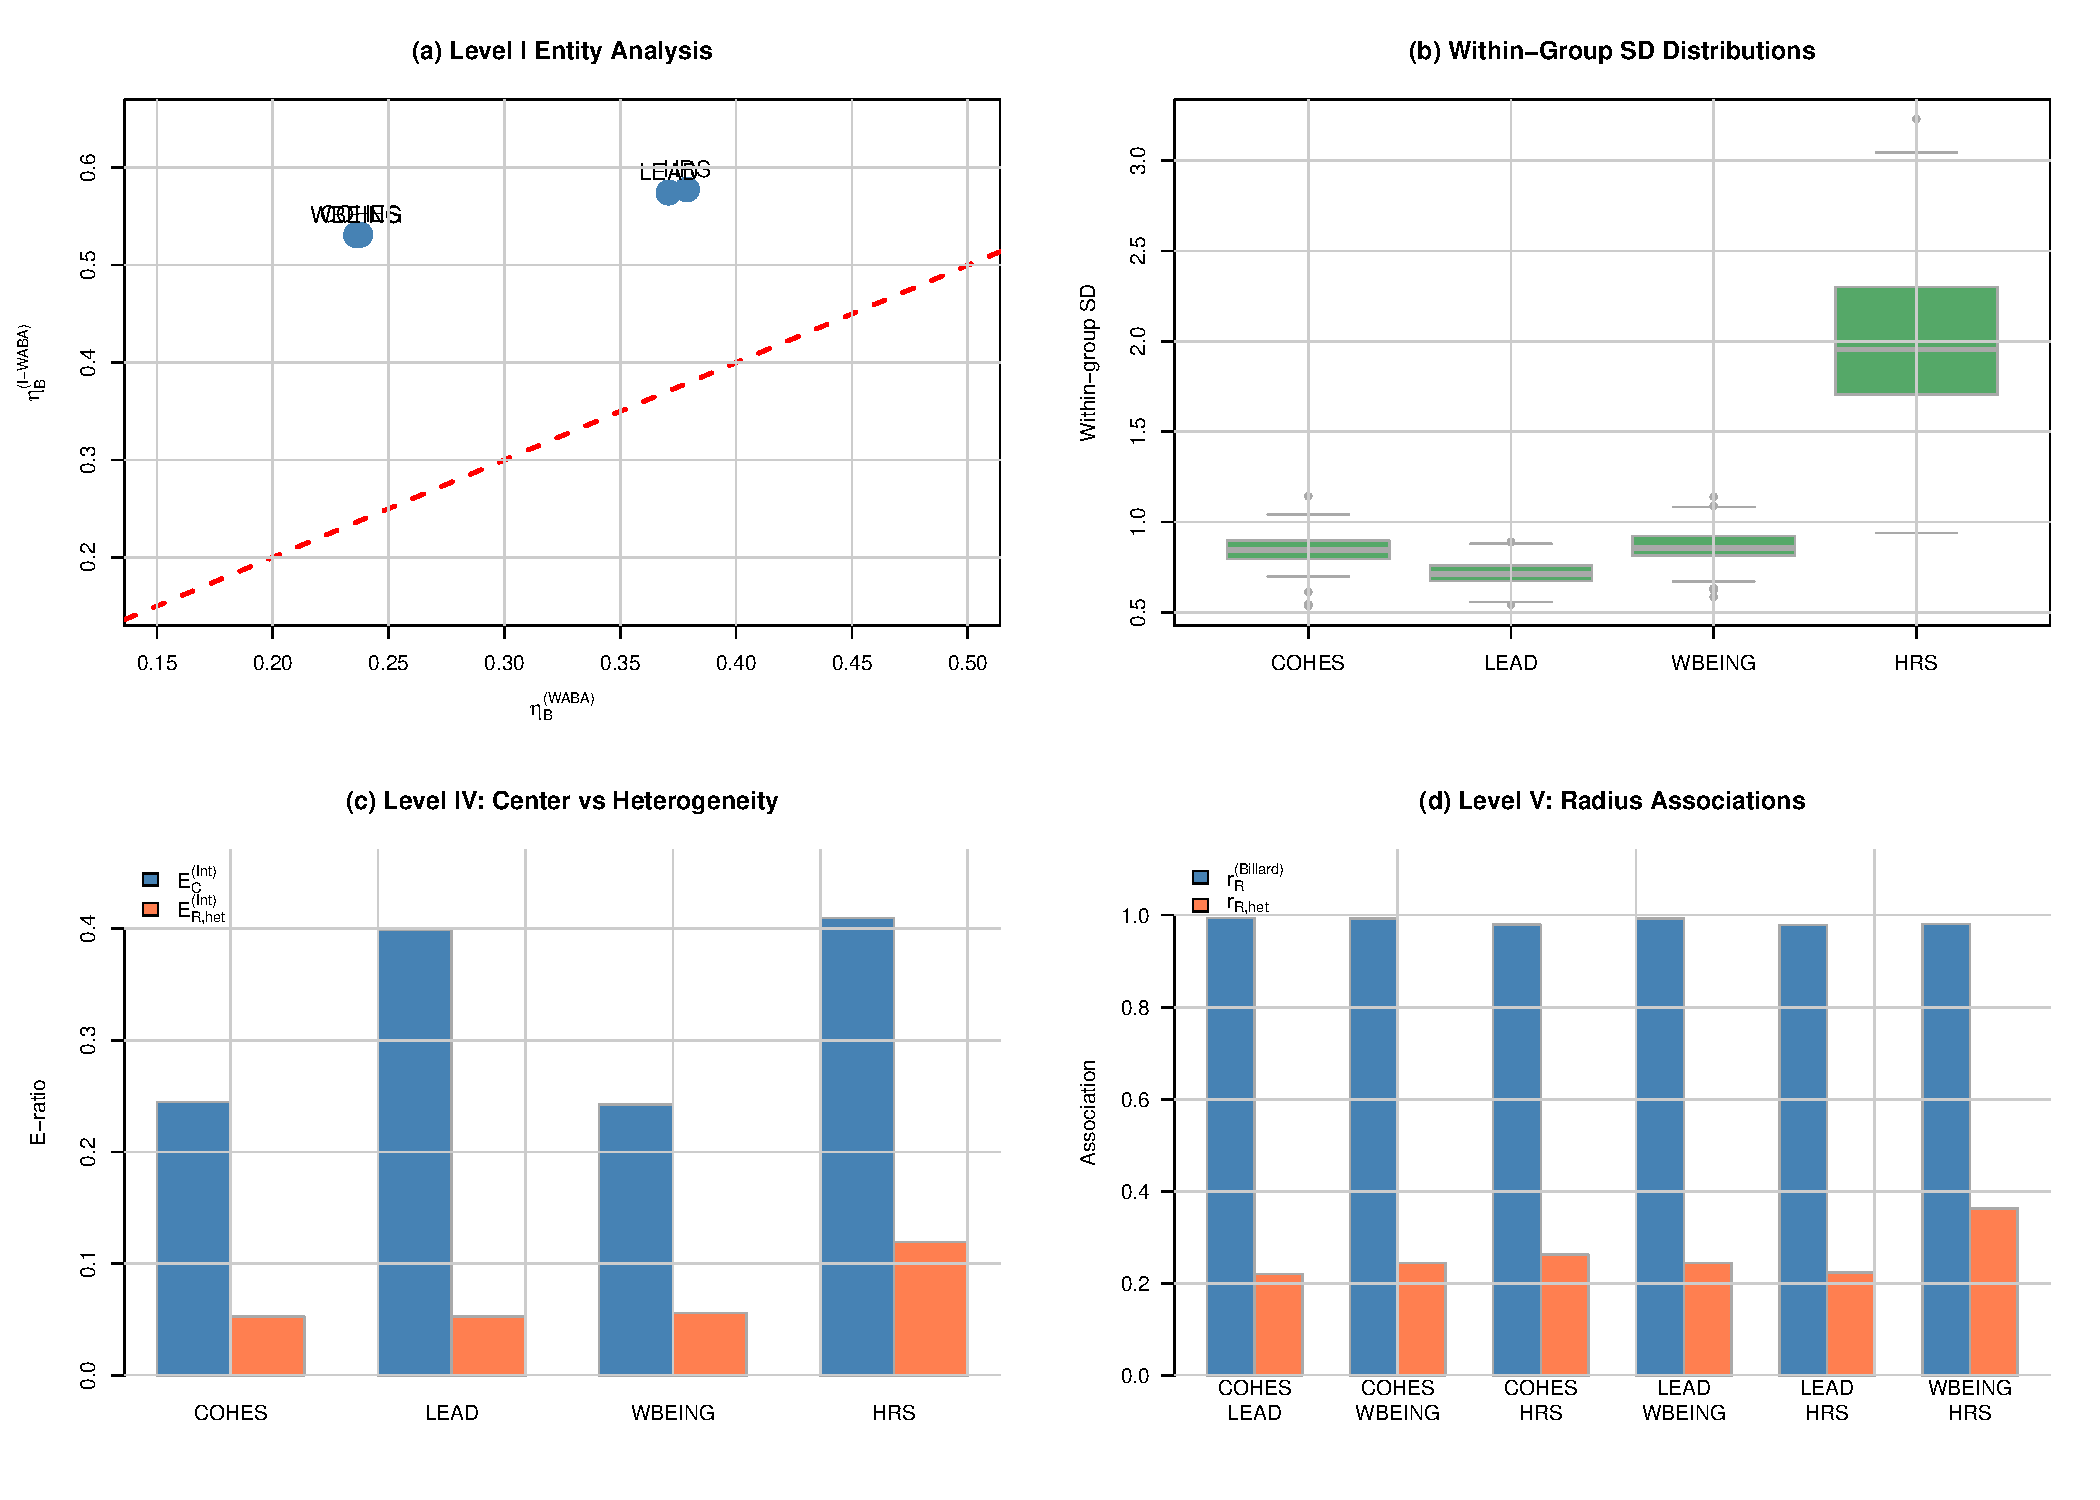
\includegraphics[width=0.95\textwidth]{fig_bh1996_analysis_v3.pdf}
	\caption{Bliese--Halverson (\texttt{bh1996}) data under the default standard-deviation radius. Panel~(a) compares the classical and interval-based between-group eta ratios \(\eta_B^{(\mathrm{WABA})}\) and \(\eta_B^{(\mathrm{I\text{-}WABA})}\) for the four variables. Panel~(b) shows the distribution of within-company standard deviations across the 99 companies. Panel~(c) contrasts the center-only E-ratio \(E_C^{(\mathrm{Int})}\) with the heterogeneity-focused radius index \(E_{R,\mathrm{het}}^{(\mathrm{Int})}\). Panel~(d) compares the magnitude-inclusive Billard radius association \(r_R^{(\mathrm{Billard})}\) with the signed centered-radius correlation \(r_{R,\mathrm{het}}\) for the six variable pairs.}
	\label{fig:bh1996_analysis}
\end{figure}

Figure~\ref{fig:bh1996_radius_sensitivity} compares the SD- and IQR-radius analyses directly. Panels~(a) and (b) show that the interval-based eta values and radius shares are fairly stable across radius definitions, whereas panel~(c) shows somewhat larger variable-level $E_{R,\mathrm{het}}^{(\mathrm{Int})}$ under the IQR radius, especially for HRS. The sharpest contrast appears in panel~(d): the signed pairwise dispersion-alignment diagnostics are markedly attenuated under the IQR radius and no longer show uniformly positive alignment. This is the most consequential sensitivity result for the \texttt{bh1996} analysis.

\begin{figure}[ht]
	\centering
	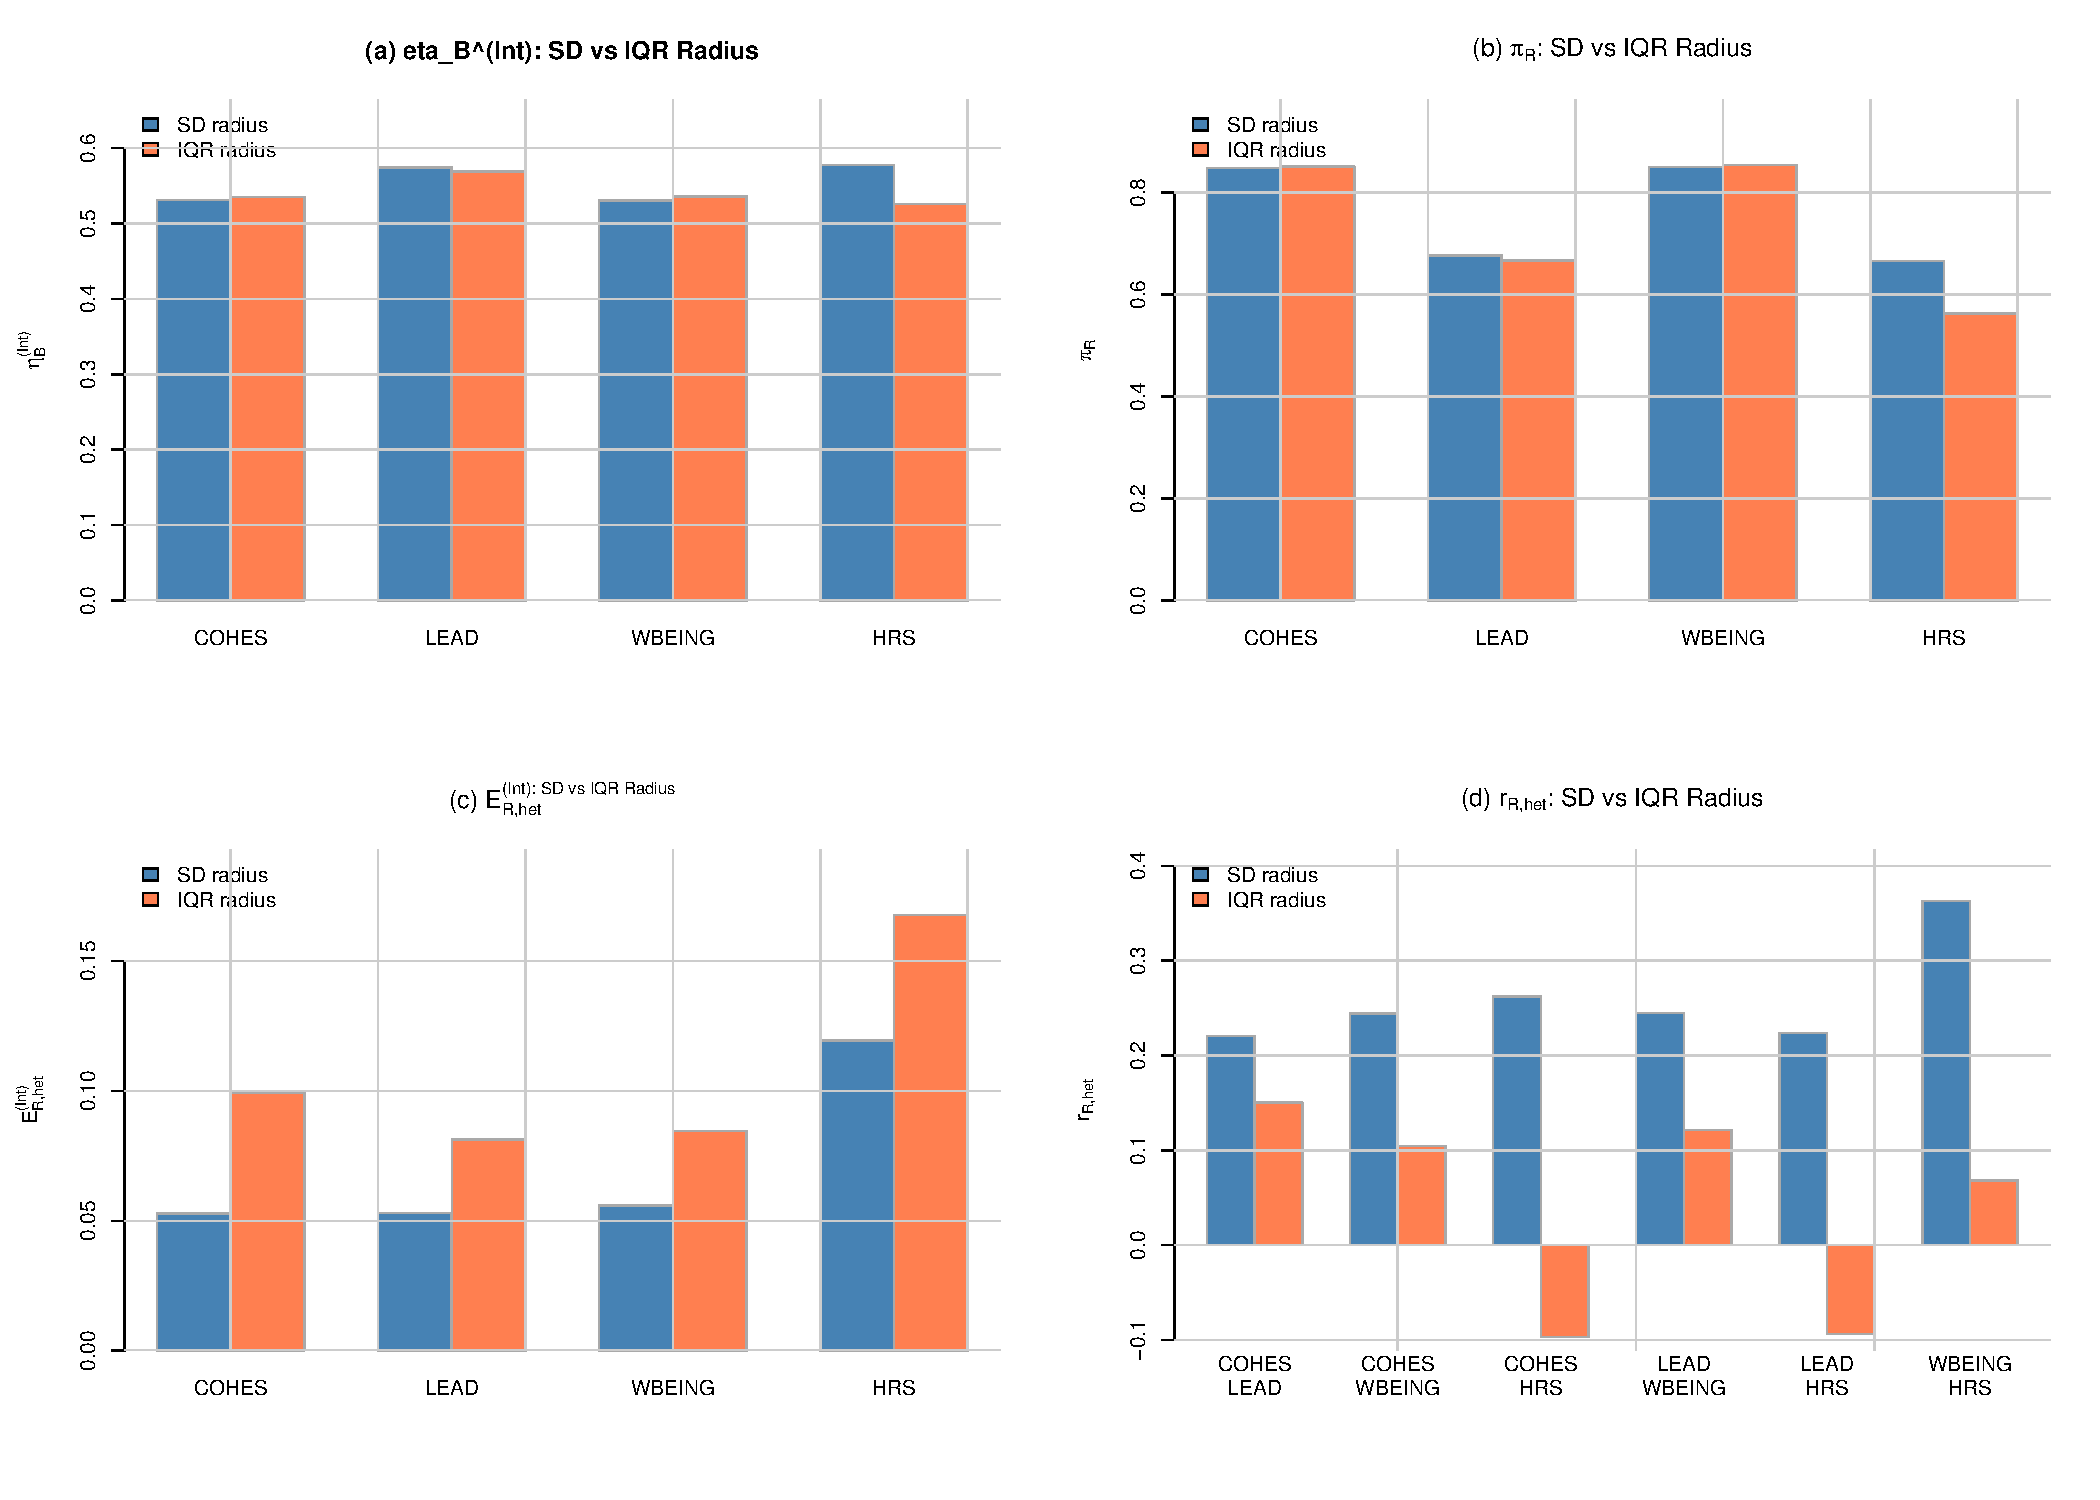
\includegraphics[width=0.95\textwidth]{fig_bh1996_radius_sensitivity_v1.pdf}
	\caption{Bliese--Halverson (\texttt{bh1996}) radius sensitivity: comparison of the default standard-deviation radius with the robust IQR-based radius \(R_{kj}=0.7413\,\mathrm{IQR}(X_j\mid \mathrm{company}=k)\). Panels show the interval-based between-group eta \(\eta_B^{(\mathrm{Int})}\), the radius share \(\pi_R\), the heterogeneity-focused radius index \(E_{R,\mathrm{het}}^{(\mathrm{Int})}\), and the signed pairwise centered-radius correlation \(r_{R,\mathrm{het}}\).}
	\label{fig:bh1996_radius_sensitivity}
\end{figure}




\subsection{Dataset 2: 14-Cancer Gene Expression ($K=14$, HDLSS)}\label{sec:data_14cancer}

The 14-Cancer dataset of \citet{Ramaswamy2001} contains $n=198$ tumor samples from $K=14$ cancer types measured on $p=16{,}063$ probes. We now analyze this dataset in four complementary branches. The primary selected-set branch uses the top 50 probes ranked by the same one-way ANOVA $F$ statistic as in the earlier draft. Because this ranking favors probes with strong between-cancer location separation, all conclusions for that branch are explicitly conditional on the selected feature set. We therefore add two sensitivity branches: a top-25 branch based on the same ranking, and a reproducible moderate-$F$ 50-gene branch obtained by sampling 50 probes uniformly from the middle 40\% of the ANOVA-$F$ ranking after excluding the top and bottom 30\%. Finally, the all-gene branch is treated as a high-dimensional screening analysis rather than as an exhaustive pairwise inferential study.

\subsubsection{Top-50 branch: descriptive decomposition}

In the top-50 branch, the interval augmentation is descriptively modest in aggregate but much more plausibly heterogeneity-driven than in \texttt{bh1996}. Because the branch is defined by the largest ANOVA $F$ statistics, it is already enriched for probes with strong between-cancer location separation; the relevant question is therefore whether the interval representation adds anything beyond that location-based preselection. The answer is yes, but modestly so. The gain is $G=1.139$, the overall radius proportion is 0.122, and the mean between-group eta rises from 0.840 under classical WABA to 0.856 under I-WABA, with no entity-level reclassifications. Thus the selected probes are already strongly between-group under the classical decomposition, and I-WABA strengthens rather than reverses that conclusion.

At the pairwise level, the interval augmentation changes the weighted decomposition only modestly in relative terms but in a consistent direction. Across the $\binom{50}{2}=1{,}225$ pairs, the mean absolute between-group correlation changes little, from 0.774 under classical WABA to 0.773 under I-WABA, but the mean absolute weighted between-group contribution increases from 0.547 to 0.567 while the mean absolute weighted within-group contribution decreases from 0.108 to 0.098. The consistency rate is already high under classical WABA (0.976) and becomes slightly higher under I-WABA (0.980); correspondingly, I-WABA classifies 1,200 of the 1,225 pairs as between-group dominant. The point is therefore not that the top-50 story changes wholesale, but that interval augmentation strengthens an already strong between-cancer structure.

The revised Level~IV diagnostics show that the radius contribution, though modest in size, is genuinely heterogeneity-driven. The mean heterogeneity-focused index is \(\bar E_{R,\mathrm{het}}^{(\mathrm{Int})}=0.329\), substantially larger than in \texttt{bh1996}, and the aggregate heterogeneity summary is \(T_{\mathrm{het}}=1.714\). The radius contribution in the top-50 branch is therefore small in aggregate size but not merely a magnitude artifact.

The revised Level~V analysis is especially important. The mean Billard radius association is 0.820, but the mean signed heterogeneity-based radius correlation is 0.520 rather than the earlier absolute-value summary of 0.569. Among the 1,225 pairs, 1,040 have positive signed \(r_{R,\mathrm{het}}\) values and 185 have negative values, with minimum \(-0.551\) and maximum \(1.000\). Thus the top-50 gene set exhibits predominantly positive but not uniform dispersion alignment. This is a substantive improvement over the old absolute-value presentation: it makes clear that shared radius magnitude and signed heterogeneity alignment are not the same phenomenon.

Figure~\ref{fig:14cancer_top50} summarizes the top-50 branch. Panel~(a) shows that all top-50 probes lie above the diagonal in the \(\eta_B^{(\mathrm{WABA})}\) versus \(\eta_B^{(\mathrm{I\text{-}WABA})}\) plot, panel~(b) shows the distribution of positive \(\Delta\eta_B\) values, panel~(c) shows marked differences in mean within-group standard deviations across cancer types, and panel~(d) shows the distribution of radius shares across the selected probes.

\begin{figure}[ht]
	\centering
	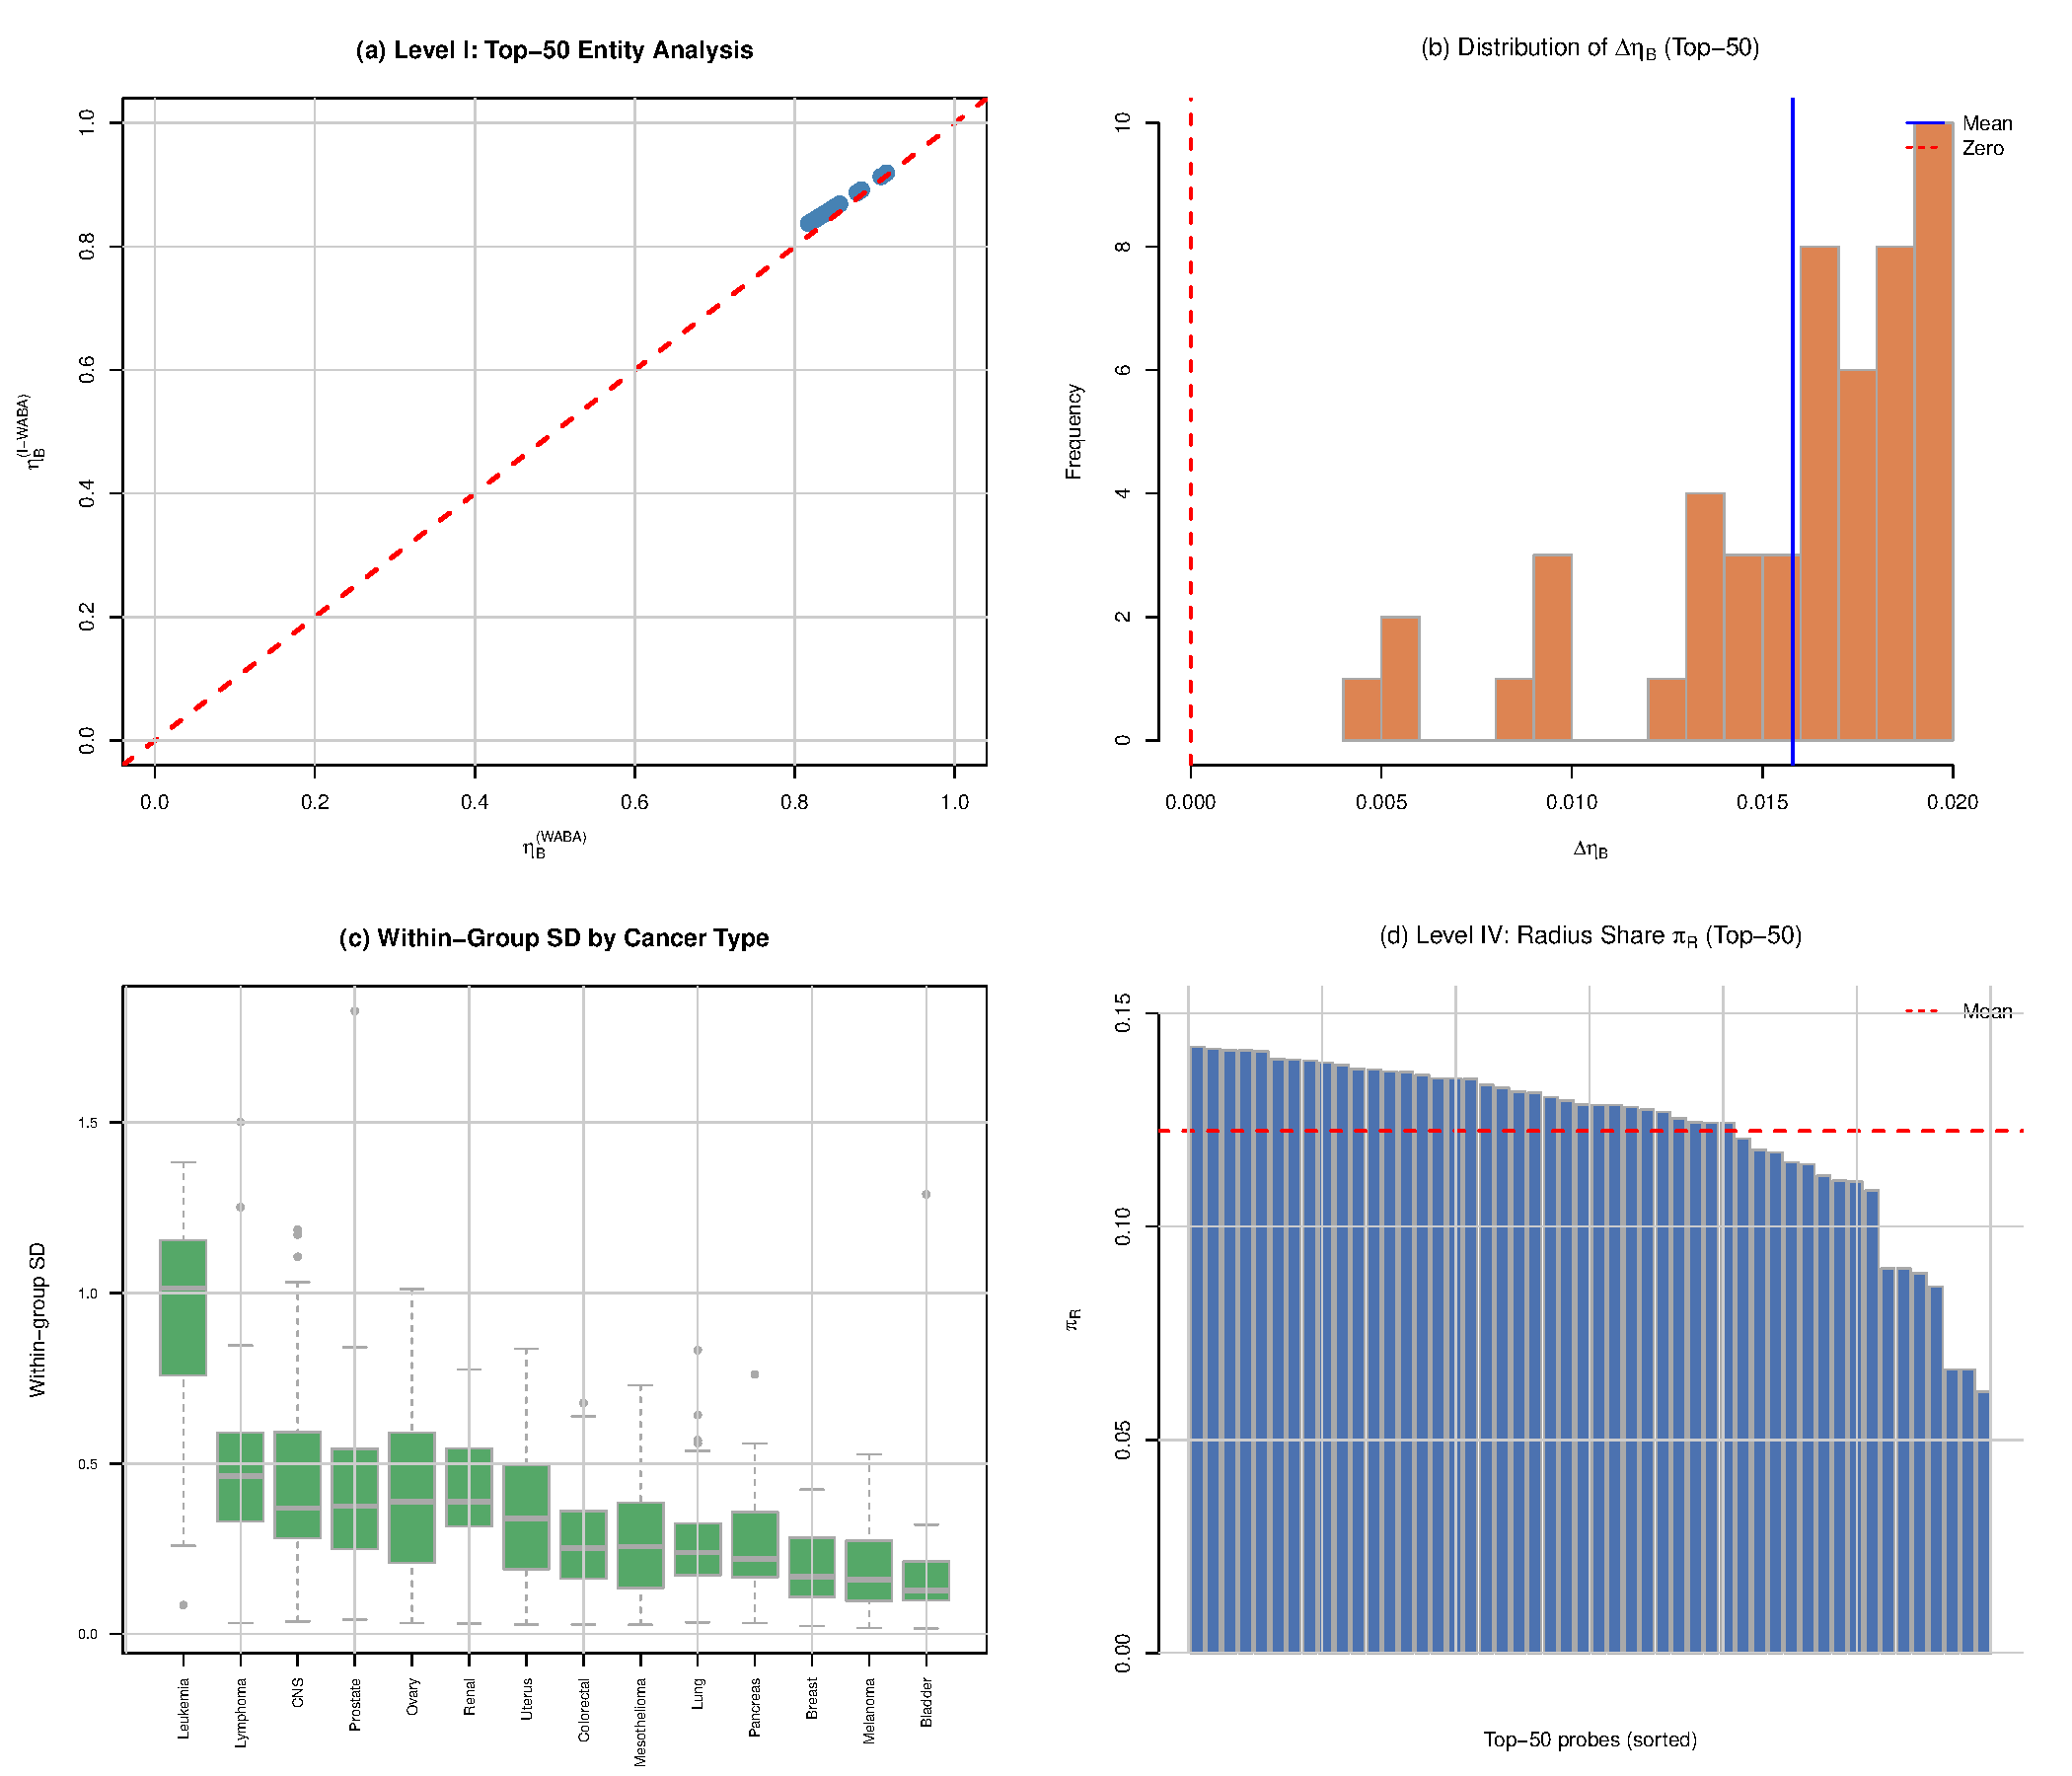
\includegraphics[width=0.85\textwidth]{fig_14cancer_top50_v3.pdf}
	\caption{14-Cancer top-50 analysis. The branch contains the 50 probes with the largest one-way ANOVA $F$ statistics after preprocessing. Panel~(a) compares \(\eta_B^{(\mathrm{I\text{-}WABA})}\) with \(\eta_B^{(\mathrm{WABA})}\); panel~(b) shows the distribution of probewise improvement \(\Delta\eta_B=\eta_B^{(\mathrm{I\text{-}WABA})}-\eta_B^{(\mathrm{WABA})}\); panel~(c) reports mean within-cancer standard deviation by cancer type; and panel~(d) shows the probe-specific radius shares \(\pi_R\).}
	\label{fig:14cancer_top50}
\end{figure}

\subsubsection{Selection sensitivity across gene subsets}

The top-25 branch supports the same selected-set story as the top-50 branch, but with slightly tighter concentration in the upper tail of the ANOVA ranking. Its gain is $G=1.121$, the radius proportion is 0.108, the mean between-group eta rises from 0.856 to 0.869, and there are again no entity-level reclassifications. At the pairwise level, 295 of the 300 pairs are between-group dominant under I-WABA, the mean signed \(r_{R,\mathrm{het}}\) is 0.426, and all 25 probes are significant after BH-adjusted Brown--Forsythe screening. Thus the qualitative top-ranked-gene conclusion is stable within the extreme upper tail of the ANOVA ranking.

The moderate-$F$ 50-gene branch gives a very different picture and is therefore the key sensitivity check for selection bias. This branch is much closer to the all-gene analysis than to the top-50 branch: $G=1.829$, the radius proportion is 0.453, the mean between-group eta rises from 0.533 to 0.651, and 49 of the 50 genes are reclassified toward stronger between-group structure. At the pairwise level, 972 of the 1,225 pairs are between-group dominant under I-WABA, the mean signed \(r_{R,\mathrm{het}}\) is 0.306, and 43 of the 50 genes are significant after BH-adjusted Brown--Forsythe screening. The moderate-$F$ branch therefore shows that the strongest top-50 narrative is not representative of every reasonable 50-gene subset; it is strongly conditioned on selecting genes with the largest mean separation.

Table~\ref{tab:sensitivity_14cancer} summarizes the four branches, and Figure~\ref{fig:14cancer_selection_sensitivity} makes the contrast visually clear. The top-50 and top-25 branches cluster together on mean \(\eta_B^{(\mathrm{Int})}\) and on the BH discovery proportion, whereas the moderate-$F$ 50-gene branch lies much closer to the all-gene branch on aggregate gain, radius share, and heterogeneity-focused strength. This is exactly the pattern one would expect if ANOVA preselection induces an upward bias toward large between-cancer location separation.

\begin{table}[ht]
	\centering
	\caption{14-Cancer selection sensitivity across four analysis branches. The top-25 and top-50 branches are conditional on upper-tail ANOVA-$F$ selection, the moderate-$F$ branch is conditional on the documented middle-band sampling rule, and the all-gene branch reports screening summaries on the full retained probe set.}
	\label{tab:sensitivity_14cancer}
	\resizebox{\textwidth}{!}{%
		\begin{tabular}{lcccccccc}
			\toprule
			Branch & $p$ & $G$ & Radius Prop. & $\bar{\eta}_B^{\mathrm{WABA}}$ & $\bar{\eta}_B^{\mathrm{I\text{-}WABA}}$ & $\bar E_{R,\mathrm{het}}^{(\mathrm{Int})}$ & Reclassified & BF--BH discoveries \\
			\midrule
			Top-50 genes            & 50       & 1.139 & 0.122 & 0.840 & 0.856 & 0.329 & $0/50$ (0.0\%)       & $50/50$ (100\%) \\
			Top-25 genes            & 25       & 1.121 & 0.108 & 0.856 & 0.869 & 0.305 & $0/25$ (0.0\%)       & $25/25$ (100\%) \\
			Moderate-$F$ 50 genes   & 50       & 1.829 & 0.453 & 0.533 & 0.651 & 0.311 & $49/50$ (98.0\%)     & $43/50$ (86.0\%) \\
			All genes               & 16{,}063 & 1.790 & 0.441 & 0.528 & 0.655 & 0.309 & $6{,}640/16{,}063$ (41.3\%) & $13{,}908/16{,}063$ (86.6\%) \\
			\bottomrule
		\end{tabular}%
	}
\end{table}

\begin{figure}[ht]
	\centering
	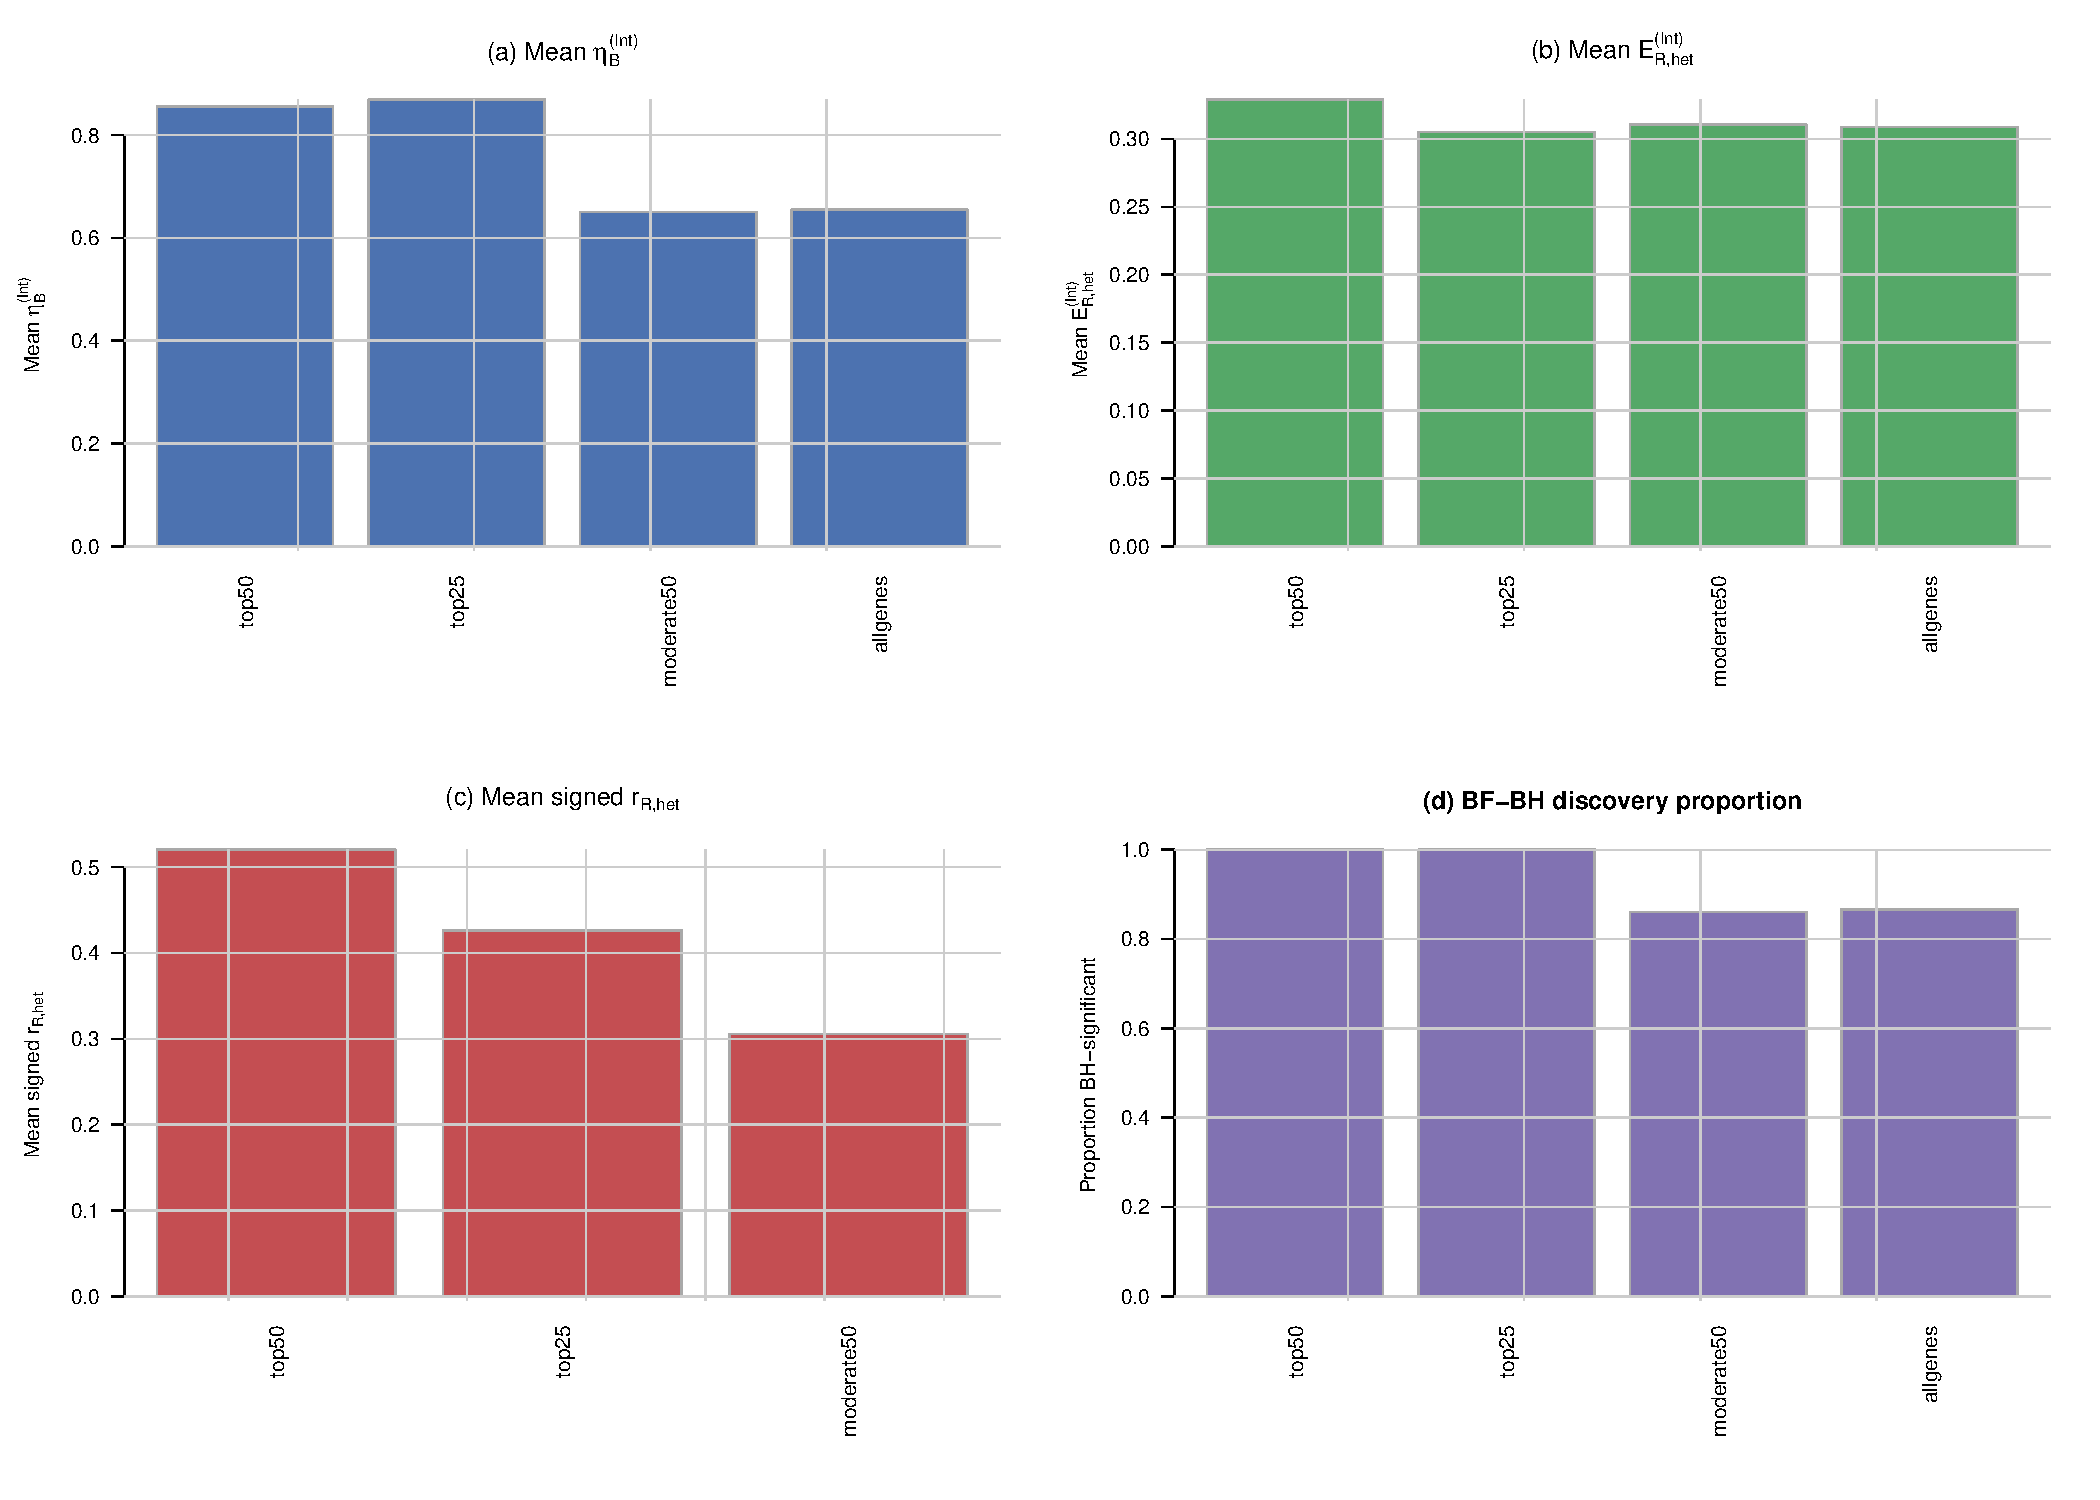
\includegraphics[width=0.95\textwidth]{fig_14cancer_selection_sensitivity_v1.pdf}
	\caption{14-Cancer selection sensitivity. Panels report branchwise comparisons of the mean interval-based between-group eta \(\eta_B^{(\mathrm{Int})}\), the mean heterogeneity-focused radius index \(E_{R,\mathrm{het}}^{(\mathrm{Int})}\), the mean signed centered-radius correlation \(r_{R,\mathrm{het}}\) for the branches with explicit Level~V summaries, and the Benjamini--Hochberg Brown--Forsythe discovery proportion.}
	\label{fig:14cancer_selection_sensitivity}
\end{figure}

\subsubsection{Top-50 branch: inferential assessment}

The inferential results for the top-50 branch are strong, though they should be interpreted as conditional on the selected feature set. Brown--Forsythe screening identifies all 50 of the 50 probes as significant after BH adjustment, indicating widespread evidence of cross-cancer dispersion heterogeneity among the selected genes.

Within-group bootstrap intervals for the aggregate summaries are all bounded away from zero in the expected direction. In particular, the 95\% bootstrap intervals for the mean interval-based eta, the mean radius share, the mean heterogeneity-focused index, and \(T_{\mathrm{het}}\) are
\[
[0.838,\;0.885],\qquad
[0.094,\;0.142],\qquad
[0.330,\;0.365],\qquad
[1.433,\;2.125],
\]
respectively. These intervals support the descriptive conclusion that the radius contribution is modest in aggregate size but clearly non-negligible and heterogeneity-driven.

The most important inferential change is that pairwise multiplicity control is now exhaustive within the selected top-50 branch rather than limited to a hand-picked subset. Across all 1,225 top-50 pairs, BH-adjusted bootstrap testing identifies 1,022 pairs significant for the dominance contrast \(\delta_{jj'}^{(A)}\) at \(q\le 0.05\) and 1,044 at \(q\le 0.10\). For the signed heterogeneity-based radius correlation, the corresponding counts are 1,025 and 1,048. Thus multiplicity-controlled pairwise support is widespread across the selected top-50 set, not merely present in a small illustrative subset. The analogous top-25 analysis is slightly smaller in absolute count but qualitatively similar, with 243 of 300 pairs significant for \(\delta_{jj'}^{(A)}\) and 249 of 300 pairs significant for signed \(r_{R,\mathrm{het}}\) at \(q\le 0.05\).

\begin{table}[ht]
	\centering
	\caption{Multiplicity-controlled pairwise bootstrap results for the 14-Cancer branches with explicit pairwise follow-up. Counts refer to Benjamini--Hochberg adjusted discoveries for the pairwise dominance contrast \(\delta^{(A)}\) and the signed centered-radius correlation \(r_{R,\mathrm{het}}\). The all-gene illustration uses the top 50 BH-significant heterogeneous genes ranked by \(E_{R,\mathrm{het}}^{(\mathrm{Int})}\); it is illustrative and does not replace the screening interpretation of the full all-gene branch.}
	\label{tab:14cancer_pairwise_fdr}
	\resizebox{\textwidth}{!}{%
		\begin{tabular}{lccc}
			\toprule
			Branch / pair set & Number of pairs & $\delta_{jj'}^{(A)}$ significant & Signed $r_{R,\mathrm{het}}$ significant \\
			\midrule
			Top-50, all pairs & 1,225 & $1{,}022/1{,}044$ at $q\le 0.05/0.10$ & $1{,}025/1{,}048$ at $q\le 0.05/0.10$ \\
			Top-25, all pairs & 300   & $243/249$ at $q\le 0.05/0.10$       & $249/255$ at $q\le 0.05/0.10$ \\
			All-gene illustration, top 50 by $E_{R,\mathrm{het}}^{(\mathrm{Int})}$ & 1,225 & $573/687$ at $q\le 0.05/0.10$ & $579/695$ at $q\le 0.05/0.10$ \\
			\bottomrule
		\end{tabular}%
	}
\end{table}

\subsubsection{All-gene branch: screening summaries and inferential scope}

The all-gene branch is intended as a high-dimensional screening analysis rather than an exhaustive pairwise inferential study. Descriptively, it resembles the moderate-$F$ branch much more than the top-50 branch. The gain rises to \(G=1.790\), the overall radius proportion to 0.441, and the mean between-group eta from 0.528 to 0.655. Every one of the 16,063 genes has positive \(\Delta\eta_B\), and 6,640 genes (41.3\%) are reclassified toward stronger between-group structure. The mean heterogeneity-focused index remains high at 0.309, and the global heterogeneity summary reaches \(T_{\mathrm{het}}=1144.47\).

The screening layer shows that this pattern is not merely descriptive. Brown--Forsythe screening yields 14,054 raw discoveries and 13,908 BH-adjusted discoveries, corresponding to 86.6\% of all genes. Together with the 3.12-fold range in mean within-group standard deviations across cancer types, this indicates that dispersion heterogeneity is pervasive across the transcriptome and not an artifact of top-50 selection.

The inferential scope, however, must remain limited. If one were to form all pairs among the 13,908 BH-positive heterogeneous genes, there would be 96,709,278 candidate pairs. Exhaustive pairwise bootstrap inference on that scale is inappropriate here. Instead, we report a restricted illustration based on the top 50 BH-significant heterogeneous genes ranked by \(E_{R,\mathrm{het}}^{(\mathrm{Int})}\). Even in that deliberately focused subset, the evidence is substantial but no longer as overwhelming as in the top-50 selected branch: 573 of the 1,225 pairs are significant for \(\delta_{jj'}^{(A)}\) and 579 are significant for signed \(r_{R,\mathrm{het}}\) at \(q\le 0.05\) after BH adjustment. The all-gene branch therefore supports strong screening-level claims about variablewise heterogeneity and interval-based eta improvement, but it should not be presented as providing exhaustive inferential certainty over all gene pairs.

\subsection{Summary of real-data results}

The two applications reinforce four general points.

First, I-WABA adds between-group information in both settings, but the source and scale of that gain differ sharply by dataset and, in the 14-Cancer study, by the feature-selection rule. In \texttt{bh1996}, the gain is very large (\(G=3.351\)), yet the heterogeneity-focused evidence is modest. In the 14-Cancer data, the top-25 and top-50 selected branches have only modest aggregate gains because they are already enriched for extreme between-cancer location separation, whereas the moderate-$F$ and all-gene branches show much larger interval-based gains. A large value of \(G\) is therefore not, by itself, evidence of strong heteroscedasticity, and in selected-set analyses it also reflects the way the features were chosen.

Second, Level~IV is essential for distinguishing magnitude-driven augmentation from genuine heterogeneous dispersion. The \texttt{bh1996} analysis shows that overall radius magnitude can dominate the augmented covariance even when cross-company dispersion heterogeneity is only moderate. By contrast, all four 14-Cancer branches have \(\bar E_{R,\mathrm{het}}^{(\mathrm{Int})}\approx 0.31\), showing that relatively modest aggregate gains in the top-ranked branches can nevertheless be supported by strong heterogeneity-focused evidence.

Third, the signed Level~V formulation materially improves interpretation. In \texttt{bh1996}, the signed and absolute-value summaries happen to agree numerically under the default SD radius because all pairwise signed values are positive, so the main gain is conceptual precision. In the 14-Cancer selected branches, however, the signed analysis changes the substantive reading: dispersion alignment is predominantly positive but not uniform, and the mean signed \(r_{R,\mathrm{het}}\) weakens noticeably when one moves from the top-ranked genes to the moderate-$F$ branch.

Fourth, the inferential additions support cautious strengthening rather than reinterpretation of the real-data section. For \texttt{bh1996}, they confirm moderate variablewise heterogeneity without overturning the descriptive entity-level conclusion of within-group dominance. For the 14-Cancer top-50 branch, they show that dispersion heterogeneity is robust at the gene level and that pairwise support remains widespread after BH control over all 1,225 pairs. For the all-gene branch, the new evidence is screening-based: multiplicity-adjusted Brown--Forsythe results indicate that heterogeneity is pervasive, but the candidate-pair count of 96,709,278 shows why exhaustive pairwise bootstrap inference should still be avoided.

\begin{table}[ht]
	\centering
	\caption{Cross-dataset summary of the interval-based augmentation. The signed heterogeneity-based radius correlation is reported only for analyses with explicit pairwise Level~V summaries.}
	\label{tab:real_data}
	\resizebox{\textwidth}{!}{%
		\begin{tabular}{lrrrrccccc}
			\toprule
			Dataset & $n$ & $p$ & $K$ & $G$ & Radius Prop. & $\bar{\eta}_B^{\mathrm{WABA}}$ & $\bar{\eta}_B^{\mathrm{I\text{-}WABA}}$ & $\bar E_{R,\mathrm{het}}^{(\mathrm{Int})}$ & $\bar r_{R,\mathrm{het}}$ \\
			\midrule
			\texttt{bh1996}                         & 7{,}382 & 4        & 99 & 3.351 & 0.702 & 0.306 & 0.554 & 0.070 & 0.260 \\
			14-Cancer, top-25 genes                & 198     & 25       & 14 & 1.121 & 0.108 & 0.856 & 0.869 & 0.305 & 0.426 \\
			14-Cancer, top-50 genes                & 198     & 50       & 14 & 1.139 & 0.122 & 0.840 & 0.856 & 0.329 & 0.520 \\
			14-Cancer, moderate-$F$ 50 genes       & 198     & 50       & 14 & 1.829 & 0.453 & 0.533 & 0.651 & 0.311 & 0.306 \\
			14-Cancer, all genes                   & 198     & 16{,}063 & 14 & 1.790 & 0.441 & 0.528 & 0.655 & 0.309 & \multicolumn{1}{c}{---} \\
			\bottomrule
		\end{tabular}%
	}
\end{table}


%%%%%%%%%%%%%%%%%%%%%%%%%%%%%%%%%%%%%%%%%%%%%%%%%%%%%%%%%%%%%%%%%%%%%%%%%%%%%%%%
%% 6. Conclusion and Discussion
%%%%%%%%%%%%%%%%%%%%%%%%%%%%%%%%%%%%%%%%%%%%%%%%%%%%%%%%%%%%%%%%%%%%%%%%%%%%%%%%
\section{Conclusion and Discussion}\label{sec:conclusion}

\subsection{Main methodological message}

We have introduced interval-based within-and-between analysis (I-WABA), an extension of classical WABA that replaces the point-valued group representation by a center--radius interval representation. The resulting framework enlarges the classical mean-based decomposition so that between-group structure can be driven by group location, group dispersion magnitude, or both. In that sense, I-WABA recasts within-and-between decomposition as a representation problem: once groups are represented by intervals rather than points, additional forms of between-group information become available.

The theoretical development yields three main ingredients. First, the classical WABA decomposition extends to the interval-based setting under Billard's covariance, producing an augmented between-group covariance with an explicit center component and a radius-product component (Theorem~\ref{thm:iwaba}). Second, at the covariance-matrix level, the interval-based between-group covariance is a positive-semidefinite enlargement of the classical between-group covariance, so interval augmentation cannot reduce the between-group component on the covariance scale (Proposition~\ref{prop:dominance}). As Remark~7 and the focal pairwise simulation summary show, this guarantee does not imply monotone strengthening of the normalized between-group correlations. Third, at the entity level, interval augmentation increases the between-group eta ratio and the E-ratio while decreasing the within-group eta ratio, clarifying how dispersion can alter between/within dominance without changing the basic decomposition logic (Proposition~\ref{prop:eta_dominance}). The structural discussion in Section~\ref{sec:role_of_K} further shows that the number of groups matters qualitatively: when $K=2$, heterogeneity-based dispersion alignment is essentially sign-only, whereas for $K>2$ the dispersion component can exhibit richer covariance structure.

At the same time, the revised simulations sharpen the interpretation of the main summaries. Because the Billard-based decomposition-scale total is not variance-preserving, the trace-based gain $G$ is best viewed as a descriptive gain on the decomposition scale rather than as a stand-alone measure of genuine heterogeneity. In settings where the classical between-group trace is near zero, the ratio $G$ can become very large even when the added signal is driven mainly by radius magnitude. For that reason, the additive trace gain $\Delta_{\mathrm{tr}}$ and the heterogeneity-focused diagnostics in Sections~\ref{sec:iwaba_IV}--\ref{sec:iwaba_V} are not merely supplementary; they are essential for interpretation. In particular, Billard's magnitude-inclusive augmentation and the centered-radius companions serve different roles: the former yields the exact algebraic enlargement, whereas the latter isolate genuine cross-group dispersion heterogeneity and signed dispersion alignment.

A further contribution of the revised framework is inferential. Section~\ref{sec:inference} develops a finite-dimensional asymptotic and bootstrap layer for the main interval-augmented summaries. The empirical group-moment vector is asymptotically normal under standard regularity conditions, smooth I-WABA summaries inherit asymptotic normality by the delta method, and the within-group bootstrap consistently approximates their sampling distributions. This yields uncertainty quantification for the entity-level and pairwise dominance contrasts together with formal assessment of dispersion heterogeneity and signed dispersion alignment. These inferential results do not replace the descriptive decomposition, but they make it possible to distinguish stable interval-based effects from finite-sample artifacts.

\subsection{Simulation evidence and inferential implications}

The simulation studies clarify when the interval-based representation is most informative and when it must be interpreted cautiously. In heteroscedastic settings, I-WABA consistently increases between-group signal relative to classical WABA. In the spread-only scenario, where group means are identical but within-group dispersions differ, the interval augmentation recovers between-group structure that is essentially invisible to the mean-based decomposition. However, the homoscedastic and complete-null controls are equally instructive. They show that a positive radius share, a large Billard radius association, or even a very large $G$ need not imply genuine cross-group heterogeneity, because overall dispersion magnitude and dispersion heterogeneity are distinct. Under the complete-null calibration, for example, the additive trace gain remains positive while the heterogeneity-focused summaries stay close to zero. This is precisely why $E_{R,\mathrm{het}}^{(\mathrm{Int})}$ and signed $r_{R,\mathrm{het}}$ are indispensable companions to $G$ and $\pi_R$.

The targeted comparator experiment also helps position the method. Brown--Forsythe is decisive for variablewise variance heterogeneity in the spread-only design and remains null-like under complete-null, whereas Welch-type mean testing stays near nominal on a per-variable basis in both settings. Thus I-WABA is not a substitute for Brown--Forsythe or Welch ANOVA. Rather, it serves a different purpose: decomposing between-group structure once within-group dispersion is allowed to contribute, and attributing that structure to location, magnitude, and centered heterogeneity.

The inferential simulations support the tiered guidance consolidated in Table~\ref{tab:sample_size_guidance}. Under balanced Gaussian sampling, dominance-contrast inference is exploratory around $n_k\approx 20$ and materially more reliable around $n_k\approx 100$, whereas signed dispersion alignment remains the more demanding target throughout. The robustness block shifts the guidance upward once the design departs from that benchmark: moderate skewness or noticeable imbalance suggests $n_k\ge 30$ as a more realistic lower bound for exploratory dominance-contrast use, and strongly skewed or highly unbalanced designs call for at least $n_k\ge 50$ together with explicit sensitivity analysis. For $r_{R,\mathrm{het}}$, the message is stricter still: strong skewness can compromise coverage even near $n_k\approx 100$, so in that regime the bootstrap layer should remain exploratory and be supplemented by robust radius checks and Brown--Forsythe screening. The $K=2$ case remains structurally special throughout: signed $r_{R,\mathrm{het}}$ should be treated as sign-only and not pooled with the graded summaries available when $K>2$.

\subsection{What the applications show}

The \texttt{bh1996} analysis illustrates substantial interval-based gain without sharply differentiated heteroscedasticity. Under the default SD radius, the mean between-group eta increases from 0.306 to 0.554 and four of the six variable pairs flip from within-group to between-group dominance, yet the mean heterogeneity-focused index is only $\bar E_{R,\mathrm{het}}^{(\mathrm{Int})}=0.070$. Brown--Forsythe testing with multiplicity adjustment flags COHES, WBEING, and especially HRS, but all four variables remain within-group dominant even under the exploratory bootstrap layer used for this large-$K$ dataset. Thus statistically significant variance heterogeneity does not imply that heterogeneity is structurally dominant in the I-WABA decomposition. The global standardization check confirms that the eta-based, E-based, and radius-share summaries are scale invariant even though the raw variance components are not, so the large variance values for HRS do not invalidate cross-variable interpretation. The IQR-radius sensitivity tells a similarly nuanced story: the entity-level and pairwise dominance conclusions are robust, but the positive signed Level~V alignment seen under the SD radius weakens substantially and is no longer uniformly positive. Hence the clearest substantive conclusion for \texttt{bh1996} is that interval augmentation captures an important company-level dispersion-magnitude component, while the evidence for coherent signed dispersion alignment is only modest and depends on the radius definition.

The 14-Cancer data show a different pattern and make the role of feature selection explicit. In the ANOVA-ranked top-50 branch, the aggregate gain is modest ($G=1.139$) because the selected genes are already enriched for strong between-cancer location separation, yet the heterogeneity-focused signal is strong (mean $\bar E_{R,\mathrm{het}}^{(\mathrm{Int})}=0.329$ and mean signed $\bar r_{R,\mathrm{het}}=0.520$), and exhaustive multiplicity-controlled pairwise follow-up shows that 1022 of 1225 pairs are significant for $\delta^{(A)}$ and 1025 of 1225 are significant for signed $r_{R,\mathrm{het}}$ at $q\le 0.05$. The top-25 branch tells essentially the same selected-set story. However, the moderate-$F$ 50-gene branch is much closer to the all-gene branch than to the top-50 branch: it has $G=1.829$, radius share 0.453, and 49 of 50 genes reclassified toward stronger between-group structure. This confirms that the strongest selected-set results are conditional on choosing genes with maximal mean separation.

In the all-gene branch, the interval-based gain is much larger than in the top-ranked branches and 41.3\% of genes are reclassified toward stronger between-group structure, while Brown--Forsythe/BH screening identifies 13{,}908 genes with evidence of dispersion heterogeneity. At the same time, those 13{,}908 genes already imply 96{,}709{,}278 candidate pairs, so exhaustive pairwise bootstrap inference remains inappropriate at transcriptome scale. The restricted all-gene illustration is therefore only an illustration, not a substitute for transcriptome-wide pairwise inference. Taken together, the 14-Cancer results show both the utility and the limits of the framework in HDLSS settings: selected-set pairwise conclusions can be very strong, but they remain conditional on the selection rule, whereas transcriptome-wide claims should remain at the level of variablewise screening unless additional structure is imposed.

\subsection{Practical guidance and relation to existing methods}

For applications, we recommend a layered workflow. Begin with the classical WABA and I-WABA decompositions together. Then inspect $G$ and the additive trace gain $\Delta_{\mathrm{tr}}$ to assess how much the interval representation changes the between-group component. Next use the Level~IV summaries to separate center-driven from radius-driven effects, and use $E_{R,\mathrm{het}}^{(\mathrm{Int})}$ together with signed $r_{R,\mathrm{het}}$ to decide whether the radius contribution reflects genuine heterogeneity and whether that heterogeneity is coherently aligned across variables. Brown--Forsythe testing is useful as a companion variablewise screen, but it targets equality of within-group variances rather than the full I-WABA null. In settings with skewness or outliers, sensitivity to the radius definition should be checked explicitly, as the \texttt{bh1996} IQR analysis demonstrates, and bootstrap inference should be treated more cautiously than under the balanced Gaussian benchmark.

\begin{table}[ht]
	\centering
	\footnotesize
	\setlength{\tabcolsep}{3pt}
	\caption{Practical sample-size guidance for the within-group bootstrap layer. Thresholds summarize the fixed-$K$ simulations in Sections~\ref{sec:sim_inference} and~\ref{sec:conclusion} and should be read as heuristic design guidance rather than sharp guarantees. Here $n_k$ denotes the typical per-group size under balance or, in unequal-group designs, the order of the smaller group sizes.}
	\label{tab:sample_size_guidance}
	\begin{tabular}{p{2.2cm}p{2.9cm}p{3.3cm}p{3.3cm}}
		\toprule
		Target & Balanced Gaussian benchmark & Moderately skewed or mildly unbalanced data & Strongly skewed or highly unbalanced data \\
		\midrule
		$\delta_j^{(E)}$ &
		$n_k\approx 20$ exploratory; $n_k\approx 100$ preferred &
		$n_k\ge 30$ as an exploratory lower bound; $n_k\approx 100$ still preferred &
		$n_k\ge 50$ only with caution and sensitivity checks; otherwise treat bootstrap intervals as descriptive only \\
		$\delta_{jj'}^{(A)}$ &
		$n_k\approx 20$ exploratory; $n_k\approx 100$ preferred &
		$n_k\ge 30$ as an exploratory lower bound; mild imbalance is less harmful than skewness &
		$n_k\ge 50$ when imbalance is the main departure; under strong skewness remain exploratory \\
		$r_{R,\mathrm{het}}$ &
		$n_k\approx 20$ unreliable; $n_k\approx 100$ preferred &
		keep $n_k\approx 100$ as the working benchmark and pair it with robust-radius sensitivity analysis &
		exploratory only under the current evidence; supplement with Brown--Forsythe screening and robust sensitivity checks \\
		\bottomrule
	\end{tabular}
\end{table}

Table~\ref{tab:sample_size_guidance} consolidates the sample-size advice scattered across the inferential and robustness simulations into a single reader-facing summary. The main practical message is that the balanced-Gaussian benchmark is the least demanding regime, while skewness is the most consequential departure. In particular, the moderate 10{:}1 imbalance design was considerably less damaging than the log-normal design, so the strongest upward adjustments in the table are driven by skewness and outlier sensitivity rather than by imbalance alone.

This also clarifies the relation to heteroscedastic mixed-effects models. Mixed models remain the primary tools when the goal is likelihood-based estimation, hierarchical prediction, or formal model comparison. I-WABA is complementary rather than competitive in that sense. Its purpose is to decompose association across levels and to attribute the between-group component to location, dispersion magnitude, and centered heterogeneity in a way that is directly comparable across variables and variable pairs.

\subsection{Limitations and future work}

Several extensions merit further study. First, the inferential development in Section~\ref{sec:inference} conditions on the observed grouping structure; the \texttt{bh1996} application, with $K=99$ and moderate-to-large company sizes, suggests that a large-$K$ or superpopulation treatment would be valuable. Second, the Billard-based augmented decomposition is algebraically convenient but not variance-preserving, and future work could investigate centered-radius-first formulations or alternative normalizations that retain closer comparability with classical totals. Third, robustness to the radius choice (standard deviation, range-based, IQR-based) and to outlying or highly unbalanced groups deserves fuller theoretical treatment. Fourth, when the grouping variable $Y$ is continuous, I-WABA currently requires discretization, and the interaction between slicing strategies and interval-based diagnostics remains open. Fifth, high-dimensional applications may benefit from regularized covariance estimation, more structured multiplicity control, and sparsity-aware pairwise procedures. Finally, one may replace interval-valued group summaries by richer distribution-valued summaries and define between-group comparisons through Wasserstein-type metrics, extending the general perspective of \citet{matsui2016d3m}.

Overall, the revised evidence supports a more precise conclusion than the original draft. I-WABA is useful not because it automatically turns dispersion differences into heteroscedastic ``effects,'' but because it reveals when within-group dispersion materially alters the between-group covariance structure and then provides the diagnostics needed to decide whether that alteration reflects magnitude, genuine heterogeneity, or coherent signed alignment. In that sense, the method extends classical WABA while preserving its basic between/within logic and making explicit a layer of group structure that the mean-only formulation cannot see.


\subsection{Software}

All analyses were conducted in R. The project archive accompanying this revision contains the scripts used for the core I-WABA functions, the simulation studies, and the two real-data analyses. A public repository containing the codebase used for this revision is available at \url{https://github.com/hanmingwu1103/I-WABA}; it includes the main simulation scripts, the real-data workflows, and a README describing the principal reproduction steps. The submitted project archive mirrors those files in case the repository changes over time.

%%%%%%%%%%%%%%%%%%%%%%%%%%%%%%%%%%%%%%%%%%%%%%%%%%%%%%%%%%%%%%%%%%%%%%%%%%%%%%%%
%% References
%%%%%%%%%%%%%%%%%%%%%%%%%%%%%%%%%%%%%%%%%%%%%%%%%%%%%%%%%%%%%%%%%%%%%%%%%%%%%%%%
\bibliographystyle{elsarticle-harv}
\bibliography{I-WABA_Wu_R4}


\end{document}
